\documentclass{article}


\usepackage{arxiv}

\usepackage[UTF8]{ctex}
\usepackage[utf8]{inputenc} % allow utf-8 input
\usepackage[T1]{fontenc}    % use 8-bit T1 fonts
\usepackage{hyperref}       % hyperlinks
\usepackage{url}            % simple URL typesetting
\usepackage{booktabs}       % professional-quality tables, 三线表
\usepackage{amsfonts}       % blackboard math symbols
\usepackage{nicefrac}       % compact symbols for 1/2, etc.
\usepackage{microtype}      % microtypography
\usepackage{lipsum}
\usepackage{graphicx}
\usepackage{color}
\usepackage{algorithm,algorithmic}
\usepackage{amssymb}
\usepackage{amsmath}
% 将参考文献加进目录中
\usepackage[nottoc]{tocbibind}
\usepackage{bm} % 使用粗体的向量
\usepackage{bbm} %使用黑板粗体的数字,如指示函数
\usepackage{subfigure}
\usepackage[table]{xcolor}
\usepackage{multirow}
\hypersetup{
    colorlinks=true,
    linkcolor=blue,
    filecolor=blue,
    urlcolor=blue,
    citecolor=cyan,
}

\usepackage{xeCJK}

\usepackage[minted]{tcolorbox}
\tcbuselibrary{skins, listings, xparse, breakable,listings}

\usepackage{pythonhighlight}
\usepackage{cpphighlight}
\usepackage{pdfpages}  
%\graphicspath{ {./images/} }

\newcommand{\tred}[1]{ {\textcolor{red}{#1}} }
\newcommand{\tbred}[1]{ {\textbf{\textcolor{red}{#1}} } }
\newcommand{\tbc}[2]{ {\textbf{\textcolor{#1}{#2}} } }


%\title{学习之旅}
\title{\mathcal{Learning LOG}}

\author{
  郭治焱 \\
  %图机器学习, 知识图谱\\
  信息科学与工程学院, 湖南大学\\
  长沙市, 岳麓区 麓山南路 \\
  \texttt{zhiyanguo@hnu.edu.cn \hspace{12pt} \href{www.zyzq.site}{www.gzyzq.site}}
  %% examples of more authors
%%   \And
%% Zixuan Lu \\
%%  School of Coumputing and Information\\
%%  University of Pittsburgh\\
%%  Pittsburgh, PA 15213 \\
%%  \texttt{ZIL50@pitt.edu} \\

  %% \AND
  %% Coauthor \\
  %% Affiliation \\
  %% Address \\
  %% \texttt{email} \\
  %% \And
  %% Coauthor \\
  %% Affiliation \\
  %% Address \\
  %% \texttt{email} \\
  %% \And
  %% Coauthor \\
  %% Affiliation \\
  %% Address \\
  %% \texttt{email} \\
}

%% defined colors
\definecolor{Blue}{rgb}{0,0,0.5}
\definecolor{Green}{rgb}{0,0.75,0.0}
\definecolor{LightGray}{rgb}{0.6,0.6,0.6}
\definecolor{DarkGray}{rgb}{0.3,0.3,0.3}
% 定义一些标记颜色,使用标记名来使用颜色
\definecolor{InfoColor}{rgb}{0,1,0}
\definecolor{ImportantColor}{rgb}{1,0,0}
\definecolor{NormalColor}{rgb}{0,0,1}
\definecolor{OtherColor}{rgb}{1,.5,0}
\definecolor{Hint}{rgb}{.99,0.93,0}


\begin{document}
\maketitle

% 定义文本显示效果
\newcommand{\tred}[1]{ {\textcolor{red}{#1}} }
\newcommand{\tbred}[1]{ {\textbf{\textcolor{red}{#1}} } }
\newcommand{\tbc}[2]{ {\textbf{\textcolor{#1}{#2}} } }

% 定义一些字体
% \newcommand{\huawenhupo}{\CJKfontspec{STHupo}}	%SimSun,宋体
%\newcommand{\heiti}{\CJKfontspec{SimHei}}
\newcommand{\lisu}{\CJKfontspec{LiSu}}
\newcommand{\kaiti}{\CJKfontspec{KaiTi}}


\newtcbox{\mybox}[1][red]{on line,
	arc=0pt,outer arc=0pt,colback=#1!10!white,colframe=#1!50!black,
	boxsep=0pt,left=1pt,right=1pt,top=2pt,bottom=2pt,
	boxrule=0pt,bottomrule=1pt,toprule=1pt}
\newtcbox{\xmybox}[1][red]{on line,
	arc=3pt,colback=#1!10!white,colframe=#1!50!black,
	before upper={\rule[-3pt]{0pt}{10pt}},boxrule=1pt,
	boxsep=0pt,left=6pt,right=6pt,top=2pt,bottom=2pt}


\newtcblisting{myjava}{listing engine=minted,
	minted style=colorful,
	minted language=java,
	minted options={fontsize=\small,breaklines,autogobble,linenos,numbersep=3mm},
	colback=blue!5!white,colframe=blue!75!black,listing only,
	left=5mm,enhanced,
	overlay={\begin{tcbclipinterior}\fill[red!20!blue!20!white] (frame.south west)
			rectangle ([xshift=5mm]frame.north west);\end{tcbclipinterior}}}
		
%%%%%%%%%%%%%%%%%%%%%% 行间代码样式 %%%%%%%%%%%%%%%%%%%%%%%%%%%%%%%%%%%
%%% 其中 minted style=algol, friendly, lovelace, pastie, tango, vs, autumn, fruity, monokai, perldoc, trac, borland, igor, murphy, rrt,vim
%%% 这些是代码的样式
%%%%%%%%%%%% mycode 环境 %%%%%%%%%%%%%%%%%%%%%%
% breakable 可换页
\newtcblisting{mycode}[2]{breakable,drop shadow,listing engine=minted,minted style=trac,
	minted language=#1,minted options={fontsize=\small,linenos,breaklines,
		numbersep=3mm},
	listing only,
	left=6mm,enhanced,title={#2},
	colframe=blue!50!black,colback=blue!10!white,colbacktitle=blue!5!yellow!10!white,
	fonttitle=\bfseries,coltitle=black,attach boxed title to top center=
	{yshift=-0.25mm-\tcboxedtitleheight/2,yshifttext=2mm-\tcboxedtitleheight/2},
	boxed title style={enhanced,boxrule=0.5mm,
		frame code={ \path[tcb fill frame] ([xshift=-4mm]frame.west)
			-- (frame.north west) -- (frame.north east) -- ([xshift=4mm]frame.east)
			-- (frame.south east) -- (frame.south west) -- cycle; },
		interior code={ \path[tcb fill interior] ([xshift=-2mm]interior.west)
			-- (interior.north west) -- (interior.north east)
			-- ([xshift=2mm]interior.east) -- (interior.south east) -- (interior.south west)
			-- cycle;} },
	overlay={\begin{tcbclipinterior}\fill[red!20!blue!20!white] (frame.south west)
			rectangle ([xshift=5mm]frame.north west);\end{tcbclipinterior}}}
%\begin{mycode}{python}{python test}
%	import pandas as pd
%	import tensorflow as tf
%	
%\end{mycode}
%%%%%%%%%%%%%%%%%%%%%%%%%%%%%%%%%%%%%%%%%%%%%%%%%%%%%%5
%%%%%%%%%%%%%%%%% commandshell %%%%%%%%%%%%%%%%%%%%%
%\newtcblisting{commandshell}{colback=black,colupper=white,colframe=yellow!75!black,
%	listing engine=minted,minted style=algol,
%	minted language=bash}

\newtcblisting{commandshell}{colback=black,colupper=white,colframe=yellow!75!black,
	listing only,left=7mm,listing,breakable, options={style=tcblatex,language=bash,numbers=left,numberstyle=\tiny\color{white!75!black}},
	every listing line={\textcolor{red}{\small\ttfamily\bfseries \$> }}
}

\newtcblisting{shell}{colback=black,colupper=white,colframe=yellow!5!black,
	listing only,left=7mm,listing,breakable, options={style=tcblatex,language=bash,numbers=left,numberstyle=\tiny\color{white!75!black}},
	minted options={fontsize=\small,breaklines,autogobble,linenos,numbersep=3mm}
	%every listing line={\textcolor{red}{\small\ttfamily\bfseries \$> }}
}

% 给环境传入参数。[1]表示有1个参数
\newtcblisting{xml}[1]{colback=yellow!5,colframe=yellow!50!black,listing only, title=#1, fonttitle=\bfseries,listing engine=minted,minted language=xml, breakable}
%%%%%%%%%%%%%%%%%%%%%%%%%%%%%%%%%%%%%%%%%%%%%%%%%%%%%%%%%%%%%%%%%%%%%
%\usemintedstyle{algol} %%全局设置
% 设置 perl 行内代码样式
\usemintedstyle[perl]{algol}
\newmintinline{perl}{showspaces} %% 行内代码样式, showspaces 代表将空格先显式的打印出来

% command 和 command* 是有区别的,command* 有命令行提示符
% 命令行示例
%\commandbox*{cd "My Documents"} changes to directory \commandbox{My Documents}.
%\commandbox*{dir /A} lists the directory content.
\DeclareTotalTCBox{\commandbox}{ s v }
{verbatim,colupper=white,colback=black!75!white,colframe=black}
{\IfBooleanTF{#1}{\textcolor{red}{\ttfamily\bfseries > }}{}%
	\lstinline[language=command.com,keywordstyle=\color{blue!35!white}\bfseries]^#2^}

% tcbuselibrary{skins}
\newenvironment{myitemize}{%
	\begin{itemize}}{\end{itemize}}
\tcolorboxenvironment{myitemize}{blanker,breakable,
	before skip=6pt,after skip=6pt,
	borderline west={1mm}{0pt}{red}}

\newenvironment{myenumerate}{%
	\begin{enumerate}}{\end{enumerate}}
\tcolorboxenvironment{myenumerate}{blanker,breakable,
	before skip=6pt,after skip=6pt,
	borderline west={1mm}{0pt}{green}}
% \begin{abstract}
% Data mining is a good way to find the relationship between raw data and predict the target we want which is also widely used in different field nowadays. In this project, we implement a lots of technology and method in data mining to predict the sale of an item based on its previous sale. We create a strong model to predict the sales. After evaluating this model, we conclude that this model can be used in normal life for future sale’s prediction. 
% \end{abstract}


% keywords can be removed
%\keywords{First keyword \and Second keyword \and More}


\vspace{\baselineskip}
\vspace{\baselineskip}
\vspace{\baselineskip}

% !Mode:: "TeX:UTF-8" 
\begin{abstract}
%-----------------------------------------------------------------------------------------
% 中文摘要
% \clearpage
% \titlespacing{\chapter}{0pt}{23mm}{5mm}



\setcounter{page}{1}
% \vskip-50mm
% {\hei
% 	\noindent 实验报告:手机相机的校正与标定 \\
% 	\noindent 姓名:杨坚 \\
% 	\noindent 学号:3117074018 \\
% 	\noindent 指导教师:袁泽剑
% }
% \vskip24mm

这份文档用于记录郭治焱在研究生期间,学习、做研究的笔记、所感所悟等。文档开始于2020年暑假(研一开学前),但是由于当时做的还比较散乱,就不当作文档的起始时间了。文档正式纪录始于\textbf{2020-09-18}。

近期逐步将一些部分的内容剥离了这个文档,将论文阅读笔记、想法分别放在了新的文档中。修改记录于\textbf{2020-10-14}凌晨。顺便感叹一下,想点子好难!

这一两周(现在是\textbf{2022-04-13})开始找实习了,人生如此多艰!我就是一个没有感情的面经生成器$\sim\sim\sim$
% \begin{center}
% \huge{{\color{red}路漫漫其修远兮, 吾将上下而求索~~~} }
% \end{center}
%% defined colors

\mybox[InfoColor]{mybox-InfoColor}
\mybox[ImportantColor]{mybox-ImportantColor}
\mybox[NormalColor]{mybox-NormalColor}
\mybox[OtherColor]{mybox-OtherColor}
\mybox[HintColor]{mybox-HintColor}
\xmybox[InfoColor]{xmybox-InfoColor}
\xmybox[ImportantColor]{xmybox-ImportantColor}
\xmybox[NormalColor]{xmybox-NormalColor}
\xmybox[OtherColor]{xmybox-OtherColor}
\xmybox[HintColor]{xmybox-HintColor}
\commandbox{commandbox}
\commandbox*{commandbox*}

\vspace{\baselineskip}
\noindent{\hei 关\hspace{0.5em}键\hspace{0.5em}词:} GNN, Machine Learning, Knowledge Graph, Recommender System, Learning To Rank, NLP, 学习记录, 科研记录

\vspace{\baselineskip}

\end{abstract}





% !Mode:: "TeX:UTF-8" 

% 中文目录
\defaultfont
\pdfbookmark[0]{目~~~~录}{mulu}
\tableofcontents
\clearpage{\pagestyle{empty}\cleardoublepage}

% 英文目录
% \pdfbookmark[0]{Contents}{econtent}
% \tableofengcontents
% \clearpage{\pagestyle{empty}\cleardoublepage}
%\section{Introduction}
%Our project is a competition on Kaggle (Predict Future Sales).


%% 插入一个学习主题
%% 注意 input 和 include 的差别,input会将导入的内容紧接着之前的内容
%% include 会重起一页插入内容

% \section{CS224W课程学习}
% %\section{CS224W课程学习}
这份文档是对CS224w课程的一个总结,该课程一共分为19个lecture,我在每个lecture的基础上进行总结,对每个lecture的知识点进行归纳,以自己理解的方式进行解释说明。课程链接点击\href{http://web.stanford.edu/class/cs224w/}{\emph{这里}}. 

\subsection{Lecture 1: Introduction; Structure of Graphs }
这一个lecture里讲的主要就是图的一些基本概念,如图的定义、传统的表示方法、图的一些属性等。这里想区分一下\textit{图和网络}:在我的理解中,图更强调一种拓扑关系,更关注点之间关系,点/边也没有各种特征或属性;网络则是“丰富版”的图,network中的结点/边是有各种各样的属性、特征的,关注的也是更深层的意义,如知识图谱、社交网络等。
\subsubsection{网络中的几个重要属性}
\textbf{Degree} \par 
\textbf{Cluster Coefficient} \par 
\textbf{Centrality} \par 
\textbf{Path} \par 
\textbf{Connected Component} \par


\subsection{Lecture 2: Properties of Networks
and Random Graph Models}

\subsection{Lecture 3: Motifs and Structural Roles in Networks}

\subsection{Lecture 4: Community Structure in Networks}

\subsection{Lecture 5: Spectral Clustering}

\subsection{Lecture 6: Message passing and Node Classification}
\subsubsection{Belief Propagation}

对于每个结点,重复下列更新,直至收敛或达到最大迭代次数:
$$
m_{i\to j}(Y_j) = \alpha \sum_{Y_i \in \mathcal{L}} \underbrace{\psi (Y_i, Y_j)\phi_i(Y_i) }_{Pr(\phi_j(Y_j) , \phi_i(Y_i)) }\prod_{k\in N_i \ j}m_{k\to i}(Y_i)  
$$

迭代结束后,结点$i$的为$Y_i$的belief为 $b_i(Y_i)$
$$
b_i(Y_i) = \alpha \phi_i(Y_i)\sum_{j\in N_i} m_{j \to i}\phi_i(Y_i), Y_i \in \mathcal{L}
$$

\subsection{Lecture 7: Graph Representation Learning}

最终的优化目标:
$$
\mathop{ max}_Z  \sum_{v \in V} log \underbrace{Pr(N_R(v | Z_v)}_{\sum_{u\in N_R(v)}Pr(u|Z_u) }   \Longrightarrow \mathop{min}_{Z} \sum_{v\in V} \sum_{u\in N_R(v)} -log\underbrace{Pr(u | Z_v) }_{=\frac{e^{z_u\top \cdot z_v}}{\sum_n z_n \top \cdot z_v} }
$$

但是计算上是很耗时的,可以采用negative sampling:
$$
log Pr(u | Z_v) \\
= log\frac{e^{z_u ^ \top \cdot z_v}}{\sum_n z_n ^ \top \cdot z_v} \\
\approx log (\sigma (e^{z_u^\top \cdot z_v})) - \sum_{i=1}^{k}log(\sigma( e^{z_{n_{i}}^\top \cdot z_v})) , n_i \sim P_V 
$$


\subsection{Lecture 8: Graph Neural Networks}

GCN: Graph Convolutional Networks
借鉴CNN的想法,网络中的卷积操作是通过聚集邻居结点的信息来完成的。关键点在于“如何聚集邻居的信息”,一中简单的方法是取均值:
$$
h_{v}^{k} = \sigma(W_k\sum_{u \in N(v)}\frac{h_{u}^{k-1}}{|N(v)|}  +B_kh_{v}^{k-1}) 
$$

在GraphSAGE中对聚集进行了泛化:

$$
h_{v}^{k} = \sigma([W_k\cdot AGG(\left\{ h_{u}^{k-1},\forall  u \in N(v) \right\}  ),B_kh_{v}^{k-1}]) 
$$

GraphSAGE在GCN的基础上对aggregator进行了泛化,但是对于一个结点的邻居都赋予了同等的权重,显然这是不合理的,我们并不能假定邻居结点的信息都是同等重要的,由此引入了注意力机制---Graph Attention Mechanism.

假设我们已经有了注意力机制 $a$。对于结点$v$的任意邻居结点$u$的权重为$\alpha_{vu}$.
这里再引入一个中间值$e_{vu}$, 表示通过$a$直接计算出的注意力值(个人叫法),即未归一化之前的权重。则有:
$$
e_{vu} = a(W_kh_v^{k-1}, W_kh_u^{k-1})
$$

$$
\alpha_{vu} = \frac{e_{vu}}{\sum_{k \in N(v)} e_{vk}}
$$

那么如何来获得一个注意力机制$a$ 呢?  \\
Multi-Head Attention.

\subsection{Lecture 9: Graph Neural Networks:
Hands-on Session}

\subsection{Lecture 10: Deep Generative Models for Graphs}

\subsection{Lecture 11: Link Analysis: PageRank}

\subsection{Lecture 12: Network Effects and Cascading Behavior}

\subsection{Lecture 13: Probabilistic Contagion
and Models of Influence}

\subsection{Lecture 14: Influence Maximization in Networks}

\subsection{Lecture 15: Outbreak Detection in Networks}

\subsection{Lecture 16: Network Evolution}

\subsection{Lecture 17: Reasoning over Knowledge Graphs}

\subsection{Lecture 18: Limitations of Graph Neural Networks}

\subsection{Lecture 19: Applications of Graph Neural Networks}

% \section{Node2vec: Scalable Feature Learning for Networks}
% %\section{Node2vec: Scalable Feature Learning for Networks}

论文主要解决了网络中结点表征学习的一个问题。首先来描述问题。\\
以优化的角度来解决结点表征的问题。在论文中具体的体现就是最大化一个似然概率。形式化定义如下:\\
$G = (V, E)$\\
$f : V \to \mathbb{R}^d$ \\
最后需要优化的式子如下:\\
$$\mathop{max}_{f}\sum_{u \in V} log Pr(N_s(u) | f(u) ) $$

论文中基于两个假设来优化该式子: \\
(1)条件独立性假设。对于结点$v$,其邻居结点之间是相互独立的;\\
(2)特征空间的对称性。简言之即任意结点对之间的影响是相等的,与顺序无关。

由于不同节点的特征会有较大偏差,按照softmax对单个的概率进行了归一化。即:\\
$$
Pr(n_i | f(u) ) = \frac{exp(f(n_i)\cdot f(u))}{\sum_{v\in V} exp(f(v)\cdot f(u))}
$$

最后得到的待优化的式子如下:\\
$$
\mathop{max}_{f}\sum_{u \in V}[ -log Z_u + \sum_{n_i \in N_S(u)} f(n_i) \cdot f(u) ]
$$
其中 $Z_u = \sum_{v\in V} exp(f(u) \codt f(v))$。但是由于直接计算$Z_u$的代价太大,采用Negative Sampling 的方法进行计算。


% \section{Semi-Supervised Classification with Graph Convolutional Networks}
% %\section{Semi-Supervised Classification with Graph Convolutional Networks}

论文主要以图卷积为基础进行半监督学习。
$$
H^{(l+1)} = \sigma(\tilde{D}^{-\frac{1}{2}} \tilde{A} \tilde{D}^{-\frac{1}{2}} H^{(l)} W^{(l)} )
$$

论文中两个tricks:\\
1)卷积时结合结点自身的信息:
$$
{\color{red}{\tilde{A} = A + I_N}}
$$

2)归一化:
$$
{\color{red} { I_N + D^{-\frac{1}{2}}AD^{-\frac{1}{2}}  \to \tilde{D}^{-\frac{1}{2}} \tilde{A} \tilde{D}^{-\frac{1}{2}} } }  
$$
其中,$\tilde{D}_{ii} = \sum_j \tilde{A}_{ij}$





% \section{GraphRNN: Generating Realistic Graphs with Deep Auto-Regressive Models}
% %\section{GraphRNN: Generating Realistic Graphs with Deep Auto-Regressive Models}

论文地址:\href{https://arxiv.org/abs/1802.08773}{https://arxiv.org/abs/1802.08773}\\
GitHub地址:\href{https://github.com/snap-stanford/GraphRNN}{GraphRNN}

论文提出了一个深度自回归(deep autoregressive)模型,用于图的生成。GraphRNN使用序列的生成概念对图的生产进行建模。为了定量地评估GraphRNN的性能,论文中使用MMD(Maximum Mean Discrepancy)的变体来衡量训练的图数据集和生成的图数据集之间的差异. 
\par 首先介绍图生成的应用。生产与真实图类似的图在很多领域都有重要的应用,例如对物理、社会进行建模,药物、分子结构的发现,构建知识图谱等。
现有的图生成的方法可以分为以下几种:\\
传统的图生成方法中,有Kronecker graphs, exponential random graphs, stocastic models等。传统的方法主要依靠手工构建特征,来生成指定特征的图,这种方法并不能直接在图数据(例如很多分子的图)中学习模型进而得到图生成模型。\\
近期也有一些深度生成模型被提出,如VAE(variational autoencoders), GAN(generative adversarial networks)\cite{kingma2014auto,goodfellow2014generative}。并且已经有一些基于深度生成模型的图生成方法,如\cite{simonovsky2018graphvae,li2018learning}。但是这些深度生成模型在生成图时依然存在一些不足,如只能从单一的图进行学习或者只能生成结点数较少的图(如少于40)。
\par 图生成问题中的几个难点:
\begin{itemize}
    \item 生成空间太大且可变。要制定具有n个结点的图需要$n^2$个值来确定边,并且结点和边的数量是不确定的。
    \item 表示不唯一。个人理解是因为图的同构性导致的。
    \item 复杂的依赖关系。边的生成并不是独立的,先后生成的边之间是存在依赖关系。\cite{li2018learning} 中提出了解决这个问题的方法,但是复杂度太高。
\end{itemize}

\par 接下来是GraphRNN 的细节。
首先先看看如何将一个图看作序列生成的过程。
对于一个给定的图$G$,图中共$n$个结点,下式中 $A^{\pi}_{ij} 为G的邻接矩阵,\pi 为结点的某个排列$。则$G$可以表示成如下形式: 
$$
S^\pi = (S^{\pi}_1,...,S^{\pi}_n)
$$
其中 $S^{\pi}_i = (A^{\pi}_{1,i},..., A^{\pi}_{i-1,i}), \forall i \in {2,...,n} $,其实就相当于邻接矩阵的第$i$列的上半部分,表示第$i$个结点与之前$i-1$个结点的连接关系。
Okay,图的序列表示解释到此为止。

\par 根据以上的解释,则一个图出现的概率$p(G)$可以表示为联合概率分布$p(G, S^{\pi})$ 关于$G$的边缘分布,令$S$表示$G$所有可能的排列,即
$$
p(G) = \sum_{S^{\pi} \in S } p(S^{\pi}) 
$$
对于某个排列$S^{\pi}$, $p(S^{\pi}}) = \prod_{i=1}^{n+1} p(S^{\pi}_i | S^{\pi}_1,...,p^{\pi}_{i-1})$, 将$p(S^{\pi}_i | S^{\pi}_1,...,p^{\pi}_{i-1})$简化表示为$p(S^{\pi}_i | S^{\pi}_{<i})$。其实意义很明显,即当前结点的某条边的概率取决于该结点已经有的边情况。

\par 现在假设已经获得了生成模型,那么如何去生成一个图呢?过程如下。
\begin{algorithm}[H]
    \begin{algorithmic}[1]
        \textbf{Input}: RNN-based transition module f_{trans}, output\ module\ f_{out}, \newline
        probability\ distribution\ \mathcal{P}_{\theta_{i}}\ parameterized\ by\ \theta_{i}, start\ token\ SOS, end\ token\  EOS, empty\ graph\ state\ h^{'} \newline
        \textbf{Output}: Graph\ sequence\ S^{\pi}
        S^{\pi}_1=SOS, h_1=h^{'}, i=1 \newline
        \textbf{repeat} \newline
            i = i+1 \newline
            h_i = f_{trans}(h_{i-1}, S^{\pi}_{i-1})\{update\ graph\ state\}\newline
            \theta_i = f_{out}(h_i) \newline
            S^{\pi}_{i} \sim \mathcal{P}_{\theta_i}\{smaple\ node\ i's\ edge\ connections\} \newline
        \textbf{until}\ S^{\pi}_i\ is\ EOS \newline
        \textbf{Return}\ S^{\pi} = (S^{\pi}_1,...,S^{\pi}_i) \newline
    \end{algorithmic}
    \caption{GraphRNN inference algorithm }
\end{algorithm}

那么剩下的就是如何去获得上面算法中即生成模型的参数了。
GraphRNN使用深度学习的方法来建模图生成的问题,不需要人为的去构建特征来生成指定特征的图,能以图数据为基础来生成类似的图,重点在于如何设计GraphRNN的模型结构。
\par 如图1所示为GraphRNN生成图的过程。
\begin{figure}
    \centering
    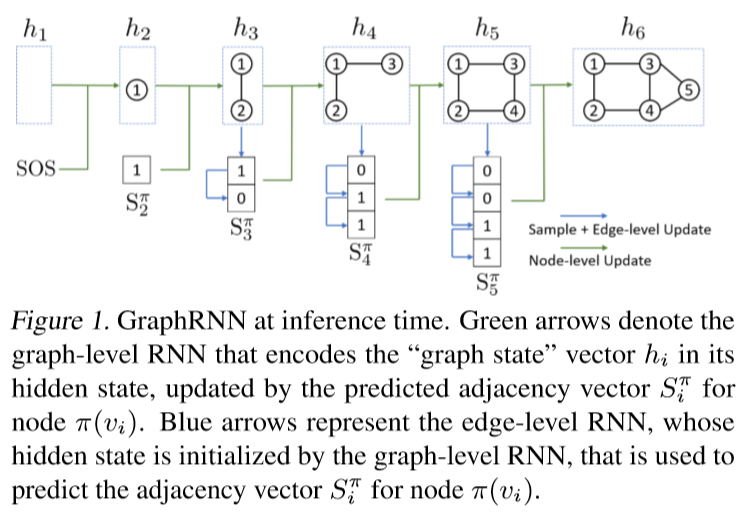
\includegraphics[width=.8\textwidth]{pics/GrpahRNN.png}
    \caption{GraphRNN生成图的过程}
    %\label{fig:my_label}
\end{figure}

GraphRNN模型是基于RNN的模型,以RNN为基础,从一个起始状态,利用RNN逐步生成图的状态,每一步向图中添加一个结点,再利用RNN生成新结点与已存在结点的连接关系,接着再向图中添加结点,重复下去直至EOS。结合之前的定义,$h_i$就是在生成过程中图的状态,它是对已经生成的图的一个encode之后的结果,每步输出$h_i$后就会将$h_i$作为另一个RNN的输入---用于生成边的连接关系的RNN。以上过程就是论文中提到的两个RNN---gaph-level RNN, edge-level RNN。
结合生成图的算法,我们可以知道有这几个部分是比较关键的:$f_{trans}, f_{out}, \mathcal{P}_{\theta_i}$。论文中对这部分都是采用神经网络来实现的,在我理解中$f_{tarns}$就是graph-level 的RNN,被$\theta_i$参数化的$\mathcal{P}_{\theta_i}$用于生成边的连接关系,即一个二进制序列。
有一个值得注意的点:$S^{\pi}_i$是一个不定长的序列,但是RNN的输入是定长的。论文中是这样处理的这个问题的:采用BFS遍历图,可以得到每个结点的依赖关系,通过对图数据集进行分析,可以得到每个节点依赖的已生成结点的数量$M$的分布,最终在训练时固定下M,即在训练时每个结点所依赖的结点数是确定的,$M$是个超参数。

\par 那么如何进行训练呢?(这部分论文中并没有进行详细的描述,代码中有较详细的过程)\\
首先要将传统格式的图数据转换为论文中定义的序列形式的图。


\par 看看这篇论文是否解决了一开始所提到的几个难点呢?
\begin{itemize}
    \item 生成空间太大且可变。个人理解论文中的graph-level和edge-level 的RNN相当于对图进行了编码,能否看作是对整个图的嵌入呢?
    \item 使用序列来表示图的生成过程,将一个确定的图的概率表示为联合概率$p(G, S^{\pi})$的边缘分布。
    \item 复杂的依赖关系。使用BFS遍历图,得到数据集中每个结点所依赖的结点的数量的分布,固定下来作为超参数。(\textbf{{\color{red}这是否可以作为一个改进的点呢?}})
\end{itemize}

\par 未来工作的方向。生成更大规模的图,高效地生成指定条件的图。


% \section{How powerful are graph neural networks?}
% 
论文地址:\href{https://arxiv.org/abs/1810.00826}{https://arxiv.org/abs/1810.00826}\\
GitHub地址:\href{https://github.com/weihua916/powerful-gnns}{powerful-gnns}

论文\cite{xu2018how}对以往的GNN模型的表现能力(区分能力)进行了理论上的分析,主要针对不同aggregation 的特点进行了分析,并针对以往的GNNs的弱点,设计了GIN(graph isomorphism network),达到了与WL sub tree相匹配的性能。论文中使用两种分类任务对以往的GNNs和GIN, WL sub tree 进行了测试:结点分类、图分类。

论文由一个问题开始讨论GNNs的区分能力。\\
给定两个图$G_1, G_2$,不同的GNNs可能会将它们(或者两图中的某两个结点)嵌入到相同的表示。这是为什么呢?这就要讨论GNNs是如何来获得结点/图的embeddings了。考虑一个通用的GNN模型:
$$
h_v^{(k)} = COMBINE(h_v^{(k-1)},  AGGREGATE({h_u^{(k-1)} | u \in \mathcal{N}_v } ) )
$$
上式中的$AGGREGATE$用来聚集邻居结点的信息(如mean, max, GRU, LSTM, GAT等),$COMBINE$则用来将聚集后的邻居结点的信息与结点自身的信息进行组合(如拼接。其实这很像一个图中的消息传播模型,现有的很多GNN模型也是基于消息传播的方法来汇聚邻居结点的信息,k层的GNN 相当与汇聚了来自k-hop的邻居的信息。({\color{red}{能否使用其他的框架来构建GNN模型呢?}})对于图$G$的embedding,是由$G$中的所有结点形成的(这涉及graph embedding的问题,参见其他论文)。
$$
h_G = READOUT(h_v^{(K)} | v \in G)
$$
再回到论文中的问题:\textbf{以往的GNN可能无法区分某些结点/图,即对不同的结点/图不能生成唯一的embeddin,不是injective的!}。根据结点/图的embedding生成的方法可以看出,关键在于$AGGREGATE, COMBINE, READOUT$,论文中将这些定义为 \textit{multi-set function},multi-set是一个可以有重复元素的集合,multi-set function就是定义在multi-set上的函数。问题就出在了GNNs使用的某些multi-set function上!
\par 论文主要对不同的AGGREGATE进行了分析,且主要分析了mean, max两种方法。
\begin{figure}
    \centering
    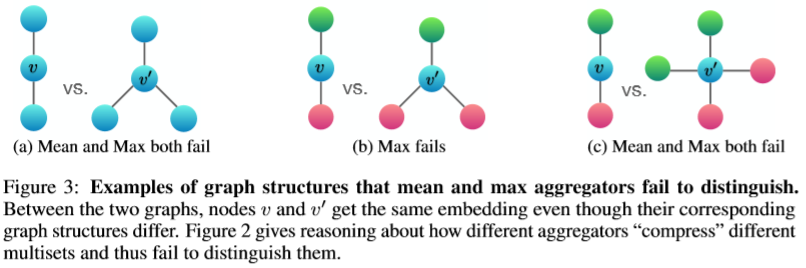
\includegraphics[width=1.\textwidth]{pics/mean-max.png}
    %\caption{Caption}
    %\label{fig:my_label}
\end{figure}
如上图所示,展示了mean, max 无法区分两个图中不同结点的邻居情况(neighborhood,即AGGREGATE后的结果是一样的)。论文中分别对mean, max的特性进行了阐述。\\
先给一个形式化的定义,假设$X$为某个结点的邻居结点集,$h(X)$就是AGGREGATE。
\paragraph{MEAN Learns Distributions} 当$h(X) = \frac{1}{|X|}\sum_{x\in X} f(x)$ 时,若对于不同的邻居结点集$X_1, X_2$,若$h(X_1) = h(X_2)$,则$X_1$和$X_2$有着相同的分布。从统计意义上来理解,相当于两个分布的均值(mean)相同。所以,当我们更需要捕捉图中某种信息的分布或者信息重复较少时,mean会有不错的效果。

\paragraph{MAX Identity "Skeleton"}(妙!) 当$h(X) = max_{x\in X}f(x)$时,若对于不同的$X_1, X_2$有$h(X_1) = h(X_2)$,则$X_1$和$X_2$有着相同的underlying set。当使用max作为AGGREGATE时,相当于对multi-set中的“重点”元素进行关注,当放在整个图中看时,相当于抽取了图中某种意义上比较“强”的结点。

\par 接下来就是重头戏 --- GIN了。
\par 论文中对结点和图的GIN定义如下:
$$
h_v^{(k)} = MLP^{(k)} ((1+\epsilon^{(k)} ) \cdot h_v^{(k-1)}+\sum_{u \in \mathcal{N}(v)} h_u^{(k-1)} ))  \newline
$$
$$
h_G = CONCAT(READOUT({h_v^{(k)} | v \in G}) | k = 0,1,...,K)
$$
看到上面的定义,你可能会疑惑,为什么GIN就比其他的GNNs好呢?这和以往的GNNs有什么区别呢?论文中对GIN使用的AGGREGATE进行了理论上的证明,证明GIN是injective的。
\par 论文中通过两个结论证明了GIN的injective性。说了几次injective了,那什么是injective呢?\\
\textbf{injective function}: 定义域中的每个不同的原像在值域中的像都是唯一的。
那么,为了让GNN有足够powerful的表现/识别能力,GNN需要尽可能精确地区分每个不同的结点/图(GNN作为以一种主要的embedding方法,高精度的表示能力能为下游任务打好基础),所以应尽量使AGGREGATE, COMMBINE, READOUT 是injective的。\\
{\color{red}证明GIN的injective}

\par 再来谈一下  Weisfeiler-Lehman (WL) graph isomorphism test 。WL isomorphism test 是用来比较两个图是否是同构的。先解释一下同构的概念。\\
抛开图同构,把同构概念单独拎出来看。对于两个系统中的对象,同构映射能够保持两个系统中的对象一一对应,且对象之间的关系也能够一一对应。图同构中,$v_1 = f(u_1), v_2 = f(u_2),u_1, u_2 \in G_1, v_1, v_2 \in G_2$,若$u_1, u_2$之间有边,则$(v_1, v_2) = g((u_1, u_2))$。\\
WL test 是通过迭代的聚集邻居的标签,每次迭代后将自己的标签和邻居们的标签映射成一个新的标签(相当于AGGREGATE后在COMBINE),迭代完成后比较两个图的标签分布(简单来说即各个标签分别有几个)是否一致({\color{red}结点的标签能否收敛呢?为什么标签的分布能用来判定是否同构呢?}),如果标签分布一致,则两个图可能是同构的。
WL subtree kernel\cite{shervashidze2011weisfeiler} 是基于 WL test的。我并没有通读论文,但是粗略看了一下图,感觉 WL subtree kernel和现在的GNN已经很像了, 对于每个结点,WL subtree kernel构建以该结点为root的树,子节点为其邻居结点,子节点的子节点是邻居结点,如此循环定义,最后以这颗树作为结点标签的依据。WL subtree kernel是目前基于聚合方式的GNNs的性能上界(证明见论文appendix)。但是WL subtree kernel并不能结合结点的信息,对于现在图中结点丰富的信息来说,这不免是有点浪费的,而且,个人认为WL subtree kernel捕捉的是图的结构(毕竟是衍生于图同构算法),或许图中的其他信息它是没有捕捉到的({\color{red}是什么信息呢?}) 

\par 关于未来的研究方向。有没有比基于聚集邻居结点信息(信息传递)方法更好的一个GNN框架呢?

关于WL test可参考的博客/非文献资料:
\begin{enumerate}
    \item \href{https://www.davidbieber.com/post/2019-05-10-weisfeiler-lehman-isomorphism-test/}{The Weisfeiler-Lehman Isomorphism Test}
\end{enumerate}




\section{Concepts about ML}
\subsection{Basics}
% 用于记录一些常见的机器学习,深度学习的概念
\subsubsection{Auto-regressive model---AR}
自回归模型,“自”体现为:使用某个变量不同时期的值(如时间序列的值)来预测该变量下一个值。AR从线性回归发展而来,假设该变量的不同步之间的值为线性关系。


\subsubsection{L1/2 regularization}

\subsubsection{mini/full-batch gradient descent}


\subsubsection{预训练,使用自编码器进行预训练}

\subsubsection{机器学习中常见的数据分布}

\subsubsection{early stopping strategy}

\subsubsection{Jacobean Hessian}


\subsubsection{Automatic differentiation} 

\subsubsection{不同的优化器原理}
可参考:\href{https://mp.weixin.qq.com/s/L9jCK5rtyq3fJZEBpLvagg}{从SGD到NadaMax,十种优化算法原理及实现}


\subsubsection{Teacher forcing}     
RNN训练时使用的一种训练方法。在训练时,使用模型的输出值用来计算误差,但是使用真实的数据作为下一次的输入。

参考资料:
\begin{enumerate}
    \item \href{https://blog.csdn.net/aws3217150/article/details/70214422}{自动微分简介}
\end{enumerate}


\subsubsection{熵、相对熵、交叉熵、互信息} 
\textbf{\checkmark 2020-10-08}\\
这些概念来自信息论\cite{6773024}。简单来说,熵指的是不确定性或者信息量,熵越大不确定越大。相对熵也叫KL(Kullback-Leibler divergence)散度,用来比较两个概率分布之间的差异。不论是熵、相对熵、交叉熵,都可以看作针对某个(或多个)随机变量,对该随机变量的概率分布的一个某种熵(熵、相对熵、交叉熵)的计算。接下来就从数学上来对其进行描述。

\textbf{熵}:先介绍自信息的概念。对于某个随机变量$X$,当$X$取值为$x_0$时的自信息为$I(x_0) = -log\ p(x_0)$,即事件$x_0$发生时所带来的信息量,如果一个事件发生的概率越大,则其带来的信息量越小。熵是自信息的均值。即$X$取任一值时所能带来的期望信息量,故$X$的信息熵$H(X) = -E_{x\sim p}I(x)$(其中p是$X$所服从的分布),即$H(X) = -\sum_{x \in X}log\ p(x)$。\textbf{因为随机变量$X$会服从某个分布,假设是$p$,则$H(X)$也可以看作是概率分布$p$的信息量的期望。}

\textbf{相对熵}:也称作KL散度。KL是在信息熵的基础上定义的,用来衡量两个分布的差异,其实由上述熵的含义可知,其实KL也可以看作是随机变量$X$,其可能服从的两个分布之间的差异。假设可能服从的两个分布分别是$p, q$,则以$q$去接近$p$时的KL散度表示为:$D_{KL}(p||q) = \sum_{x \in X} p(x) log\ \frac{p(x)}{q(x)} = E_{x\sim p} log\ \frac{p(x)}{q(x)}$。经过化简可得$D_{KL} = -H(p) + \sum_{x \in X}p(x)log\ q(x)$。

\textbf{交叉熵}:\label{ce}cross-entropy,与KL散度相似,也是用来衡量随机变量$X$可能服从的两个分布$p, q$之间的差异的。其数学上的定义为:$Cross-Entropy(p, q) = -E_{x\sim p} log\ q(x) = - \sum_{x \in X}p(x)log\ q(x)$。很显然,交叉熵比KL散度多了一个$H(p)$,即$Cross-Entropy(p, q) = D_{kL}(p || q) + H(p)$。

机器学习中常使用交叉熵,既然KL散度和交叉熵都可以达到相同的目的,那为什么不使用KL散度呢?在机器学习中,上述的分布$q$常作为数据的真实分布,而$q$作为数据的预测分布,此时$H(P)$则可以视作一个常数(因为给定数据后,其真实分布是确定的),在优化模型的参数时,$H(P)$并不会对参数的优化做出贡献(不会影响优化过程),故使用交叉熵即可。

\subsubsection{metric learning} 
度量学习。学习如何衡量两个对象之间的相似度/距离。


\subsubsection{xavier innitializatino} 
Xavier\cite{pmlr-v9-glorot10a}一种参数初始化方法。神经网络模型的参数初始化时很重要的,对模型最终的效果、收敛速度都有很大的影响。

\subsubsection{批训练的过程,原因}
在训练神经网络时,通常训练数据都是很大的,无法一次性加载进内存。可以把数据分为很多个batch,使用每个batch训练模型后再进行参数调整。

\subsubsection{Contrastive loss, Triplet loss} 
都是一种损失函数。

Triplet loss用于训练差异较小的数据,常用于人脸识别中。以这种函数为损失函数时,输入的一个样本是一个三元组(anchor, positive, negative),anchor是随机选择的一个样本,而positive和negative分别于anchor为同类/异类数据。在学习时,Triplet loss的目的就是让anchor的表征与positive的表征尽量靠近,与negative的表征尽量疏远。那么对于一个样本来说,Triplet loss写成公式: $$\mathcal{L} = max( ||f(a)-f(p)||_2^2 - ||f(a) - f(n)||_2^2 + \alpha )
$$
公式的含义也很明显,尽量使类内数据相近,类间数据相离。

Contrastive loss是对比损失,也叫zero-one损失,主要用来处理孪生网络中的paired data的关系。通常Contrastive loss的输入是两个样本,且各自都有一个标签,Contrastive loss的目标就是:如果两个样本同类,则loss更小,否则loss更大。写成公式:
$$
\mathcal{L} = d_{ij}^2 \cdot Y_{ij} + (1 - Y_{ij} )max(margin - d_{ij}, 0)^2
$$
其中,$d_{ij}$就表示样本i, j之间的距离,这个可以有多种形式的定义,$Y_{ij}$表示样本i, j的标签是否相同,margin是一个阈值,如果$d_{ij}$超过阈值则应该尽量把它们划分开。

\subsubsection{Batch Normalization}
在神经网络的训练过程中,前一层的输出相当于后一层的输入,当对参数进行更新的时候,前一层的输出会发生变化,可能前一层---后一层的输入的分布就发生了变化,这会降低模型的收敛速度或使得模型难以收敛。为了解决这个问题,BN通过对每一层的输出进行标准化,使其分布尽量稳定下来,加快模型的收敛速度。实际情况在进行BN时,可能是在通过激活函数之间进行BN或者在通过激活函数后再进行BN。通常是在激活函数之前进行BN,因为当输入较大时,通常激活函数的变化都较小,梯度变化不明显,故在激活函数之间就对数据进行BN,使其分布尽量稳定。


\subsubsection{判别模型、生成模型}
\begin{itemize}
	\item 判别模型:直接对判别函数或者条件概率分布函数进行建模,不考虑样本的产生模型,直接研究预测模型
	\item 生成模型:学习联合概率密度$P(Y, X)$,然后求出条件概率分布$P(Y|X) = \frac{P(X, Y)}{P(X)}$,不仅要求出联合分布,还要求出训练数据的分布$P(X)$({\color{red}{不一定要计算$p(X)$,因为对于同一个样本,计算它属于不同分类时,其$p(X)$是一样的,对判别没有帮助}})。生成模型表示了输入$X$产生输出$Y$的生成关系
\end{itemize}

对于生成式模型,可以这样理解:\\
$p(x | y) = p(y)p(x | y)$表示的是,从$p(y)$中采样一个$y$,然后根据$p(x|y)$采样一个$x$。生成式模型希望找到那个能够使$p(x, y)$最大的$y$。1


生成模型从统计的角度表示数据的分布情况。判别模型不能反映训练数据本身的特性,但它不断寻找不同类别之间的最优分类面。

也可以从 \textbf{决策函数$Y=f(X)$或条件概率分布$P(Y|X)$} 的角度来看待判别模型和生成模型:
从数据中学习一个分类器时,希望通过给定的输入$X$输出相应的$Y$。这个模型的一般形式为:
\begin{itemize}
	\item 决策函数$Y=f(X)$:输入一个$X$就输出一个$Y$,可以将$Y$于阈值比较得到$X$的类别
	\item 条件概率分布$P(Y|X)$:输入一个$X$,输出$X$属于各个类的概率,如$P(c_1 | X), P(c_2 | X)$。取其中最大的作为$X$的类别
\end{itemize}
实际上$P(Y|X)$是隐含了或者说可以转化为决策函数形式$Y=f(X)$的。例如,将条件概率分布改写为$Y = \frac{P(c_1 | X)}{P(c_2 | X) }$。

参考资料:\href{https://blog.csdn.net/fishmemory/article/details/51711114}{判别模型(Discriminative model)和生成模型(Generative model)}、\href{https://developers.google.cn/machine-learning/gan/generative?hl=zh-cn}{Background: What is a Generative Model?}。


\subsubsection{Koopman分析}


\subsubsection{Model Collapse}
模型坍塌,很形象啊,就是模型出现了一个漏洞,不管你输入什么东西都会漏进这个洞里。

这个主要出现在GAN的模型中。GAN通过生成器G和判别器D来使G捕捉到真实数据的分布。在训练GAN模型时会出现model collapse的现象,即G只捕捉到了真实数据的部分分布。为什么会这样呢?简单的介绍一下:当G捕捉到了真实数据的部分分布后,被D识破了,于是G就改变,从某个分布跳到了另外的分布,并且抛弃了原来的分布,于是就成了“猫鼠游戏”,D一直追着G跑,G最终并没有完全捕捉到真实数据的分布。参考:\href{https://blog.csdn.net/SPARKKKK/article/details/72598041}{GAN——ModeCollapse}。

\subsubsection{Inductive Bias}
归纳偏置,使用某个算法解决问题时所基于的假设,类似于贝叶斯中的先验(prior),与先验不同,归纳偏置在学习过程中不会被更新,而先验会不断被更新。机器学习中常见的归纳偏置:奥卡姆剃刀、CNN中的局部性、KNN中假设相似样本在特征空间中也是相邻的、SVM假设好的分类器应该是类别边界距离最大的等。

\subsubsection{Covariate Shift}
指机器学习中训练集和测试集样本分布不一致的现象。通常在机器学习中假设训练数据和测试数据的分布是一致的,通过训练数据习得的一组最优参数能否使得模型在测试数据上也有很好的表现呢?当训练集和测试集的分布不是那么相似时,covariate shift就出现了。

怎么解决呢?训练集和测试集的分布不一致导致模型的参数不能很好地应用到测试集上,可能是测试集中地某些样本在训练集中被“轻视”或“过度重视”了,因此可以通过附加一个权重来解决该问题。可参考:\href{https://blog.csdn.net/mao_xiao_feng/article/details/54317852}{covariate shift现象的解释}。

\subsubsection{关于交叉熵损失函数的一点理解}
交叉熵损失函数可以从多个角度进行理解。从概率论的角度,在极大似然概率估计中,希望参数能够使得已有样本出现的概率最大。

在分类任务中,由于不同样本是有标签的,样本出现的概率应该与标签对应,例如p表示1样本出现的概率,则1-p表示0样本出现的概率,那么对于1样本极大化的应该是p,对于0样本极大化的应该是1-p。

样本的极大化后的概率取对数后为相加的形式。则对于一个样本,其极大化的表示可以写成$log p$ (1样本),或者$log(1-p)$( 0样本)。如果用一个统一的式子表示的话,可以写成$y log p + (1-y) log(1-p)$,其中y取0或1。

通常是对损失函数最小化,所以可以在极大化的表示前加个符号就变成了交叉熵损失函数:$- y log p - (1-y) log(1-p)$。将一个batch里的样本的损失累加起来就是常见的形式了。并且,在用模型计算p时,p通常通过一个函数来表示$f(x)$,x即为输入的样本,$f(x)$可以是各种机器学习模型,如逻辑回归、神经网络等。

除了从极大似然的角度来理解交叉熵损失函数,当然也可以直接从交叉熵\ref{ce}的角度来理解。

\subsubsection{关于CNN的一点理解}
于DNN相比,CNN有两个特点:1)局部感知;2)权值共享。

局部感知。在CNN中每个Feature map中的一个值只于上一层的Feature map的一小部分有关。如果将CNN展开成DNN的形式,则一层中的一个神经元的输入只是上一层的某几个神经元。与全连接不同,全连接将上一层的所有信息作为输入,捕捉整体的信息。但局部感知以某个区域内的信息作为输入,捕获上一层数据中存在的局部信息 --- 特定的模式。

权值共享。CNN中的每一个filter都可以得到一个Feature map,同一个Feature map中的元素之间通过同一个filter卷积得到。或者说,同一层的神经元由一个filter产生,共享一套参数。
见Fig.\ref{fig:share_weight}。图来源于李宏毅老师的ppt。有一点需要注意,CNN模型的输入图像可能是单通道的也可能是三通道的,此时\textbf{每个filter不仅由长和宽还有深度},filter的深度与图像的通道数是相等的,所以一般来说有多少个filter就有多少个Feature map。

\begin{figure}[h]
	\centering
	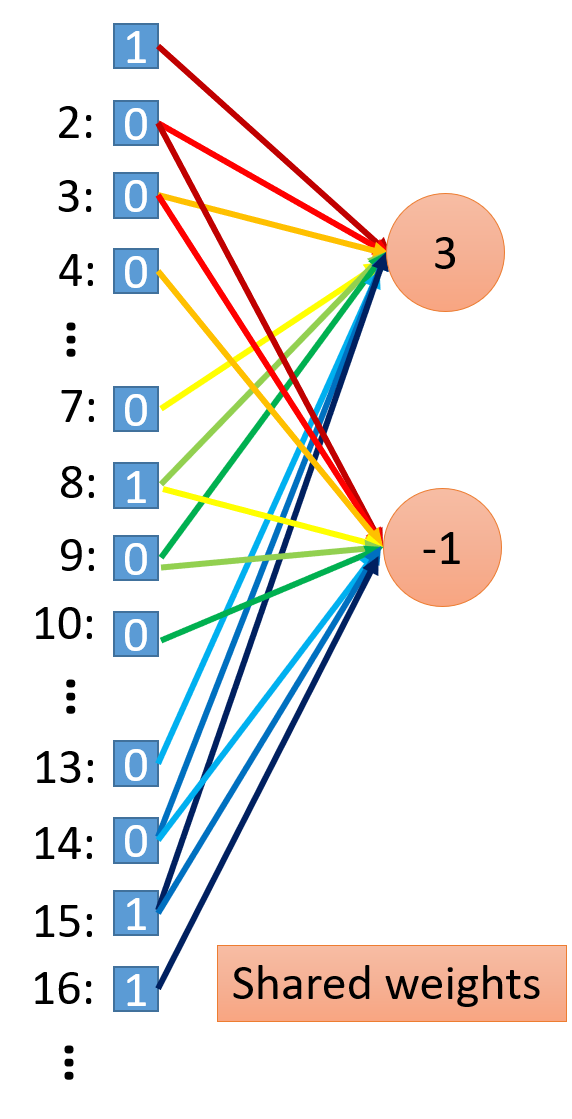
\includegraphics[width=.3\textwidth]{pics/share_weight.png}
	\caption{CNN的权值共享}
	\label{fig:share_weight}
\end{figure}

CNN的应用非常广泛,不仅是图像,在Speech、NLP等很多领域都有非常多的应用。在决定是否要使用基于CNN的模型时,需要考虑:1)数据中存在一些较小的模式,这些模式经常出现在数据中 --- 对用卷积核;2)模式与整个数据相比比较小,更大的语义信息是由很多小的模式组成的;3)进行pooling时不会破坏数据本来的含义。

在探索CNN到底学习到了什么的时候,可以在训练好模型后,通过不断优化输入的数据,来检验是什么样的输入使得基于CNN的模型中的神经元能够得到最大的激活 --- 什么样的输入使神经元最兴奋。这些主要涉及到对CNN的解释和可视化。

\subsubsection{DL中的不可微操作}

\subsubsection{batch normalization、layer normalization}

\subsubsection{Global Max Pooling}

\subsubsection{Attention机制与CNN}

\subsubsection{学习率衰减与参数正则化}

\subsubsection{深度学习中常见的参数初始化方法}
\paragraph{Glorot initialization}

\subsubsection{机器学习中常用的算法指标及其应用场景}

% Please add the following required packages to your document preamble:
% \usepackage{multirow}
% \usepackage[table,xcdraw]{xcolor}
% If you use beamer only pass "xcolor=table" option, i.e. \documentclass[xcolor=table]{beamer}
\paragraph{Accuracy, Recall, Precision, F-score}

$ACC = \frac{TP + TN}{TP+FN+TN+FP}\quad R = \frac{TP}{TP+FN}\quad P = \frac{TP}{TP+FP}\quad F(\beta) = (1 + \beta^2)\frac{P \cdot R}{\beta^2 P + R}$。混淆矩阵(Confusion Matrix)见表.\ref{tab:confusion_mat}。F-score是对R,P的一个综合评价,$\beta$度量了R 相对于 P的重要性,可以理解为$\beta = \frac{importance(R) }{importance(P)}$,则表示$\beta$越大,我们越看重R。

\begin{table}[h]
	\centering
	\caption{二分类混淆矩阵}
	\label{tab:confusion_mat}
	\begin{tabular}{|c|l|l|}
		\hline
		\multicolumn{1}{|l|}{}                          & \multicolumn{2}{c|}{Actual class (observation)}                                                                                   \\ \hline
		& tp (true positive) Correct result                          & fp (false positive) Unexpected result                                \\ \cline{2-3} 
		\multirow{-2}{*}{Predicted class (expectation)} & \cellcolor[HTML]{68CBD0}fn (false negative) Missing result & \cellcolor[HTML]{68CBD0}tn (true negative) Correct absence of result \\ \hline
	\end{tabular}
\end{table}

\paragraph*{关于$Precision$,$Recall$的选择?}这几个指标在很多任务中都有应用,,但是不同的指标侧重于不同的方面,比如P、R都有不同的侧重,但看一个指标是比较片面的,并不能反映出模型真实的效果。有可能P很高,但是R很低,而在一些场景下R是很重要的。

比如在金融风控等领域,我们希望算法能够尽量识别出所有有可能有风险的用户,这时候就侧重于Recall,即希望算法把所有的正样本(通常有危险的,需要被找出来的被标记为正样本)都筛选出来,即使将所有样本都标为正(这是Recall=1)。因为这种情况下,可能漏掉一个正样本带来的代价是极大的,通常筛选完之后还需要交给人工进行判断。类似的场景还有癌症检测,将一个没有癌症的判断为癌症没有很大关系,但是将一个有癌症的判断为没有癌症则是很严重的,会出人命的!!!

又比如在垃圾邮件分类中,我们可能更侧重于Precision。我们希望算法在识别垃圾邮件时不要把正常邮件错分了,这个时候希望Precision尽可能高,即使将所有样本标为负也没关系(TP=0时可认为Precision=1),或者说算法只把自己十分确信为垃圾邮件的标为正,尽量降低FP,即尽量不要把正常邮件视为垃圾邮件,不然错过了offer那可咋整!!!

通常,将需要识别出的类别,或者简单的说坏的一类为正样本,为什么呢?因为好的漏掉一般不会产生啥大的影响,但是坏的跑了课就不行了!当然,也需要不同场景下选择合适的指标!!!

我们是贪心的,因此就有了一些综合的指标,比如F-score。
Precision是以被分类的所有样本为分母,Recall则是以原本所有的positives元素为分母。二者之间并没有建立直接联系,如果一个分类器,Precision很高但是Recall很低,或者Recall很高但是Precision很低,这两种分类器都是不好的,都是我们不希望的。所以我们采用F1-Score来建立Precision和Recall的联系。

\textbf{在数学中,调和平均数是永远小于等于算术均值平均数的,当用于求两个数的平均数时,如果直接用算术平均作为结果,那么两数之间的差异将被大的值削平,而调和平均数则不会极大削平这种大的差异,得到的结果更倾向于小的值}。

\paragraph{Micro-F1 \& Macro-F1}基本的F1使针对二分类任务而言的,在多分类中中,Micro-F1和Macro-F1是两种求多类别F1均值的方式。
\begin{itemize}
	\item Micro-F1:分别计算每个类别的$TP, FN, FP$,再求整体的$Recall$,$Precision$,再以整体的$P, R$来求$F1$,得到Micro-F1。在计算公式中考虑到了每个类别的数量,所以适用于数据分布不平衡的情况;但同时因为考虑到数据的数量,所以在数据极度不平衡的情况下,\textbf{数量较多的类(即常见的类)会较大的影响到F1的值}
	\item Macro-F1:分别计算每个类别的F1,再求平均,得到Macro-F1。没有考虑到数据的数量,所以会平等的看待每一类(因为每一类的precision和recall都在0-1之间),\textbf{会相对受高$Precision$和高$Recall$类(即稀有的类)的影响较大}
\end{itemize}
$Micro-F1$公式如下所示:
$$
\begin{aligned}
	 Recall_{m i} &=\frac{\sum_i TP_{i}}{\sum_i TP_{i} + \sum_i FN_{i}} \\
	Precision_{m i} &=\frac{\sum_i TP_{i}}{\sum_i TP_{i} + \sum_i FP_{i}} \\
	Micro-F1 &= \frac{ Recall_{m i} \times Precision_{m i}}{Recall_{m i}+ Precision_{m i}}
\end{aligned}
$$
$Macro-F1$如下所示:
$$
Macro-F1 &=2 \frac{ \sum_i F1_i}{N}
$$


\paragraph{ROC、AUC}接收者操作特征曲线(recevier operating characteristic curve),用于反映一个而分类器的灵敏度(sensitivity)和特异度(specificity)之间的关系。
$$
\begin{aligned}
	Sensitivity &= \frac{TP}{TP + FN}\\
	Specificity &= \frac{TN}{TN + FP}
\end{aligned}
$$
其中Sensitivity也就是TPR(True Positive Rate),也就是Recall,Specificity是TNR(True Negtive Rate)。ROC的横坐标是$1 - Specificity$,即FPR(False Positive Rate),纵坐标是Sensitivity。横坐标表示的是负样本中被预测为正样本的比例,纵坐标表示的是正样本中被预测为正样本的比例。

ROC如Fig.\ref{fig:roc}所示。

\begin{figure}[h]
	\centering
	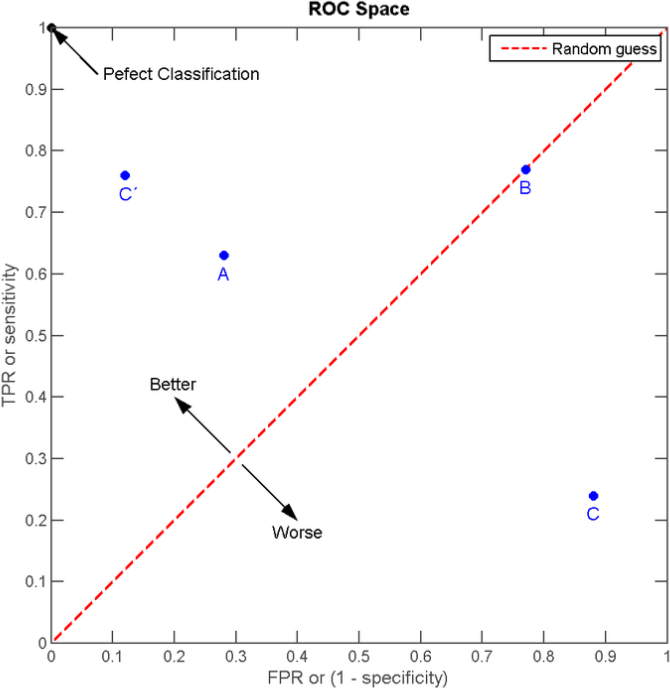
\includegraphics[width=.6\textwidth]{pics/roc.png}
	\caption{ROC}
	\label{fig:roc}
\end{figure}
ROC的绘制过程:对于一个二分类问题,使用一个分类器对样本集进行预测后,可以得到每个样本属于正样本的概率,此时我们还需要一个阈值来确定那些为正样本。每选取一个阈值,就可以得到一个(TPR,FPR)数值对。当阈值从1到0不断减小时,被确定为正样本的样本数不断增大,其中TP和FP都会不断增大,由于正负样本的数量是固定的(即TPR,FPR的分母是固定的),则TPR和FPR都会不断增大。那么,
\begin{itemize}
	\item 当阈值为1时,(几乎)所有样本都为负样本,则TPR约为0,既然都为负样本那么FP也为0,则FPR也为0
	\item 当阈值为0时,所有样本都为正样本,那么肯定所有的正样本都找出来了,则TPR为1,由于所有样本都预测为正样本,那么肯定所有的负样本都预测为了正样本,则FPR为1
\end{itemize}
因此,在阈值从1到0的过程中,(TPR,FPR)不断增大,从坐标(0,0)到(1,1),如Fig.\ref{fig:threshold}所示,Fig.\ref{fig:threshold}上部分为负样本为正样本的概率的分布图(即横坐标为正样本概率值,纵坐标为对应的样本数量),下部分为正样本为正样本的概率的分布图,可见,当阈值为$B$时,大部分正样本都被分为了正样本(TP),小部分负样本被分为了正样本(FP)。由Fig.\ref{fig:roc-threshold}可见,当阈值减小时,(TPR,FPR)的变化过程。

\begin{figure}[h]
	\centering
	\subfigure[阈值变化与预测正负样本的分布]{
		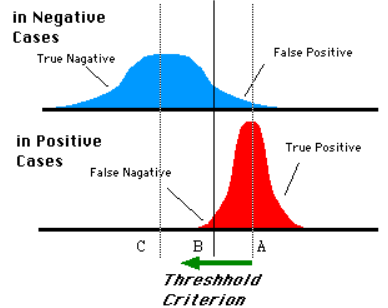
\includegraphics[width=7cm]{pics/threshold.png}
		\label{fig:threshold}
	}
	\quad
	\subfigure[阈值变化与ROC]{
		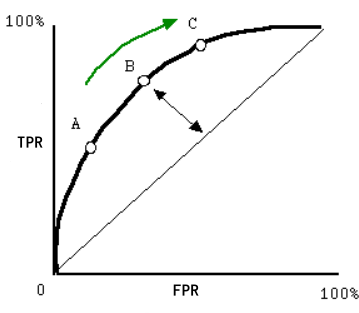
\includegraphics[width=7cm]{pics/roc-threshold.png}
		\label{fig:roc-threshold}
	}
	\caption{阈值变化}
	\label{fig:threshold-change}
\end{figure}
ROC是一个曲线,那怎么作为一个指标呢? --- 取ROC与坐标轴围成的面积,即\textbf{AUC(Area Under Curve)}。由于ROC的绘制过程,我们希望当阈值为接近0时,TPR尽量高,FPR尽量低(其实不管阈值为何值,都希望有这个效果),一个好的分类器的ROC的AUC应该尽量大。

AUC的含义:随机挑选一个正样本、一个负样本,分类器分别给出一个分数,正样本的分数大于负样本的分数的概率。\tbc{red}{强烈推荐}-相关证明:\href{http://vividfree.github.io/%E6%9C%BA%E5%99%A8%E5%AD%A6%E4%B9%A0/2015/11/20/understanding-ROC-and-AUC}{\tbc{red}{理解 ROC 和 AUC}}。

\textbf{为什么要用ROC/AUC呢?}\newline
因为ROC曲线有个很好的特性:当测试集中的正负样本的分布变化的时候,ROC曲线能够保持不变。在实际的数据集中经常会出现类不平衡(class imbalance)现象,即负样本比正样本多很多(或者相反),而且测试数据中的正负样本的分布也可能随着时间变化。roc曲线不变原因:TPR和FPR是实际label内部的操作,看混淆矩阵和tpr、fpr计算公式,无论实际label比例怎么变化,tpr、fpr计算公式都是在实际为p或者n的内部计算的

\textbf{如何使用ROC来选择模型?}\newline
当我们有多个分类器时,给定一个数据集,可以得到多条ROC曲线,那么怎么来选择模型呢?一个很直观的想法是直接比较AUC。但是在不同场景下,我们要结合更看重的指标选择模型。如Fig.\ref{fig:roc-cmp}所示,当ROC不交叉时,可以直接选择AUC高的,当ROC交叉时则需要慎重考虑了。当需要高的Sensitiviy时,选择A,需要高Specificity(即低FPR)时选择B。


\begin{figure}[h]
	\centering
	\subfigure[ROC不交叉]{
		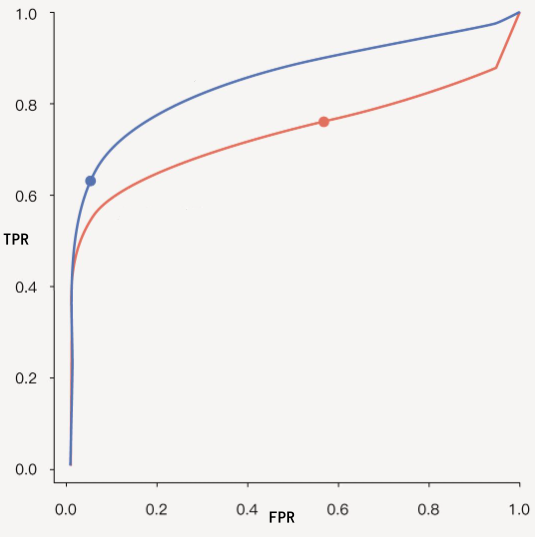
\includegraphics[width=7cm]{pics/roc1.png}
		\label{fig:roc1}
	}
	\quad
	\subfigure[ROC交叉]{
		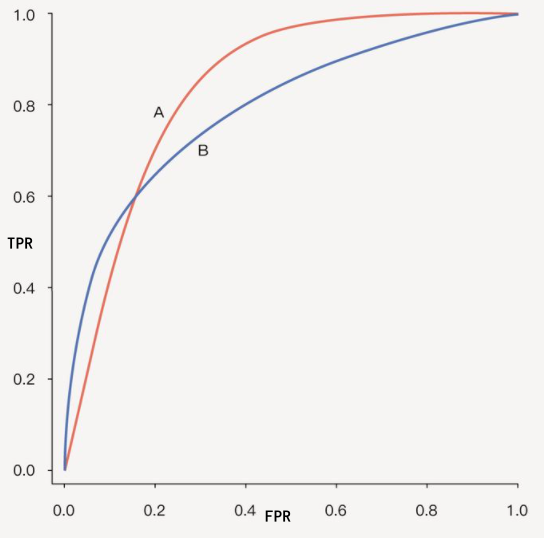
\includegraphics[width=7cm]{pics/roc2.png}
		\label{fig:roc2}
	}
	\caption{ROC比较}
	\label{fig:roc-cmp}
\end{figure}

参考资料:
\begin{itemize}
	\item \href{https://blog.csdn.net/pipisorry/article/details/51788927}{分类模型评估之ROC-AUC曲线和PRC曲线}
	\item \href{https://zh.wikipedia.org/zh/ROC%E6%9B%B2%E7%BA%BF}{ROC曲线}
\end{itemize}


\paragraph{mIoU}
Mean Intersection over Union(MIoU,均交并比),为语义分割的标准度量。其计算两个集合的交并比,在\textbf{语义分割}的问题中,这两个集合为真实值(ground truth)和预测值(predicted segmentation)。令$p_{ij}$表示实际类别为$i$,预测类别为$j$的数量,则
$$
mIoU = \frac{1}{C} \sum_{i=1}^{C} \frac{p_{ii}}{ \sum_{j=1}^{C} p_{ij} + \sum_{j=1} p_{ji} - p_{ii} }
$$
如下图Fig.\ref{fig:miou}所示:
\begin{figure}[h]
	\centering
	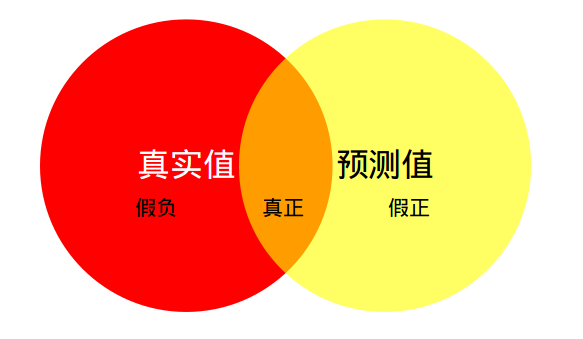
\includegraphics[width=.6\textwidth]{pics/miou.png}
	\caption{mIoU}
	\label{fig:miou}
\end{figure}
在\textbf{语义分割}中,被分类的对象为每个像素,真实标签为该像素所属的类别,预测标签为预测的类别。计算时,可以先计算出混淆矩阵,将对角线上的元素的值之和除以混淆矩阵中所有元素的和,再除以类别数就是mIoU了。注意,在实际计算中,要注意除零的情况。

\paragraph{Dice}
有Dice系数和Dice loss之分。
Dice系数是一种集合相似度度量函数,通常用于计算两个样本的相似度,取值范围在[0,1],计算公式如下:
$$
dice(x, y) = \frac{2|x \cap y|}{|x| + |y|}
$$
在\textbf{语义分割}中,$x, y$可以分别代表预测的分割结果、真实的分割,分别以矩阵的形式表示。那么,计算模型的分割效果可以为:
$$
dice(pred, ground) = \frac{2(pred \cdot ground).sum()}{pred.sum() + ground.sum()}
$$
其中,$\cdot$和\textit{.sum()}分别表示矩阵的逐元素乘积、逐元素求和。
Dice loss则是:$1 - dice(pred, ground)$,Dice loss 首次在VNet中提出。

在图像分割实践中,可以用Dice loss或者交叉熵损失函数作为目标函数,但是由于交叉损失函数的梯度形式更优,更倾向于选择交叉熵损失函数。
Dice Loss特点:
\begin{itemize}
	\item 训练误差曲线非常混乱,很难看出关于收敛的信息。尽管可以检查在验证集上的误差来避开此问题
	\item Dice Loss比较\textbf{适用于样本极度不均的情况},一般的情况下,使用 Dice Loss 会对反向传播造成不利的影响,容易使训练变得不稳定
	\item Dice对mask的内部填充比较敏感
	
\end{itemize}
作为Dice loss的一个替代,可以使用cross entropy loss。原因:
\begin{center}
	使用交叉熵做损失函数时,在反向传播时,计算得到的梯度的形式是类似于(p-t)的,其中$p, t$分别是预测值和标签。而dice loss,如果将其写成$\frac{2pt}{p^2+t^2}$ 或 $\frac{2pt}{p+t}$的形式,则在反向传播时,梯度大概时这个样子的: $\frac{2t(t^2-p^2)}{(p^2+t^2)^2}$ 或 $\frac{2t^2}{(p+t)^2}$。这样的梯度有什么问题呢?当$p, t$都很小时,梯度可能会变得很大,这也是\textbf{dice loss在训练过程中不稳定的原因}了。
\end{center}



\paragraph{Rand Error}
Rand Error是以Rand Index(兰德系数)为基础的。Rand Index用于衡量两个数据簇之间的相似性。Rand Index的定义:
对数据点集进行分类时,用a表示实际为同一类,预测时也为同一类的数据点对(pair)的数量,b表示实际为不同类,预测时也为不同类的数据点pair的数量,则
%\binom{n}{k}\qquad\mathrm{C}_n^k
$$
RI(Rand Index) = \frac{a + b}{\mathrm{C}_n^k}
$$
Rand Error定义为:
$$
RE = 1 - RI
$$
RE可以用于衡量图像分割算法的效果。可以参考:\href{http://www.otlet-institute.org/wikics/Clustering_Problems.html#toc-Subsection-4.1}{Rand Index计算}。

\paragraph{Hausdorff 距离} 可以用于衡量两个点集之间的距离,定义如下,其中$\boldsymbol{X}, \boldsymbol{Y}, d(x, y)$表示两个点集和点之间的距离度量函数:
$$
d_{H}(X, Y) = \max (d_{X Y}, d_{Y x}) = \max \left\{\underset{x \in X}{\max } \min _{y \in Y}d(x, y),\quad \max _{y \in Y} \min _{x \in X} d(x, y)\right\}
$$
\textbf{Dice缺陷在于对边界的刻画不敏感},注意力主要集中在mask的内部。而Hausdorff距离作为形状相似性的一种度量,能够为Dice做出较好的补充。
\begin{figure}[h]
	\centering
	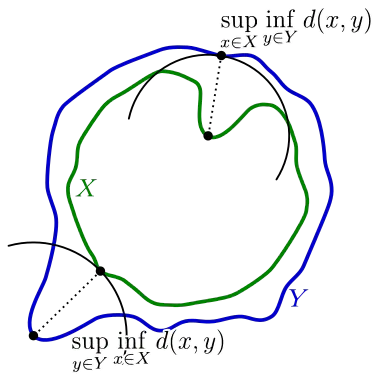
\includegraphics[width=.5\textwidth]{pics/Hausdorff distance.png}
	\caption{Hausdorff Distance}
	\label{fig: hausdorff distance}
\end{figure}

\paragraph{MRR}
Mean Reciprocal Rank,常用来衡量搜索算法效果的指标,目前被广泛用在允许返回多个结果的问题,或者目前还比较难以解决的问题中(由于如果只返回top 1的结果,准确率或召回率会很差,所以在技术不成熟的情况下,先返回多个结果)。在这类问题中,系统会对每一个返回的结果给一个置信度(打分),然后根据置信度排序,将得分高的结果排在前面返回。核心思想很简单:返回的结果集的优劣,跟第一个正确答案的位置有关,第一个正确答案越靠前,结果越好。定义如下:
$$
MRR = \frac{1}{|Q|} \sum_{i=1}^{|Q|} \frac{1}{rank_i}
$$
其中$Q$为查询集合,$rank_i$是第$i$个查询的结果集中正确结果的排名。

\paragraph{AP}
Average Precision,平均精确率。对于二分类问题,给定样本真实标签$\{y_1, ..., y_n\}$和模型预测的正样本置信度$\{c_1, ..., c_n\}$,计算AP:
\begin{enumerate}
	\item 按照置信度从大到小对样本进行排序,令排序后的样本的置信度为$\{c_1, ..., c_n\}$
	\item 令 $i=1$,重复执行:
	\begin{enumerate}
		\item 以$c_i$为阈值,得到预测的正负样本,即前$i$行预测为正样本,之后的均为负样本
		\item 计算当前阈值下的Recall和Precision
		\item $i += 1$
		\item 当$i > n$则结束循环
	\end{enumerate}
	\item 排序后的每个样本都对应一个(Recall, Precision)对,即$\{(r_1, p_1), ..., (r_n, p_n)\}$
	\item 上一步得到的Recall列表$\{r_1, ..., r_n\}$中的元素$r_i$与$r_{i-1}$做差,设$r_0 = 0$,则可以得到$\{d_1, ..., d_n\}$,其中$d_i = r_i - r_{i-1}$
	\item 求和:$AP = \sum_{i=1}^n d_i \cdot p_i$
\end{enumerate}
如Fig.\ref{fig:ap}所示,该表是按照置信度排序后的样本,correct列表示该样本的真实标签,P、R列是按照上述方式计算出来的Recall和Precision。
\begin{figure}[h]
	\centering
	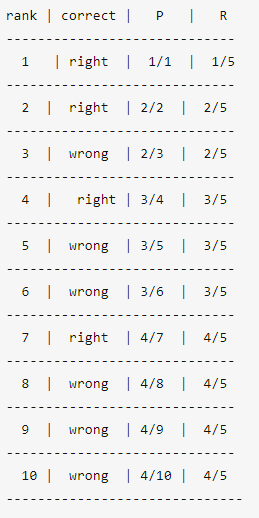
\includegraphics[width=.3\textwidth]{pics/AP.png}
	\caption{AP计算示例}
	\label{fig:ap}
\end{figure}

\paragraph{MAP}
Mean Average Precision,是AP的均值。AP通常是针对单个类别而言的,当有多个类别时,分别计算每个类别的AP,再进行算术平均。

\tbc{red}{注意:}AP和MAP常用在目标检测和信息检索领域中。
\begin{itemize}
	\item 目标检测领域中,对于一个类别,可能会检测出多个检测框,每个检测框可以根据IoU来判断检测框的真实标签是1还是0(针对一个类别的检测而言,\tbc{green}{因为目标检测中的Ground Truth也是一个边界框,所以不需要和边界框完全一致才作为正样本,只要IoU大于一定阈值即可}),每个检测框还对应一个置信度。此时即可按照上述方式计算该类别的AP
	\item 在信息检索领域,对于一个查询$q$,通常希望模型能够给出top K个结果(\tbc{red}{有序的})。若$q$真实的有序搜索结果列表为$\{d_1, ..., d_m\}$,则可以对这K个结果的标签,由于模型的输出已经是排好序的,故可以直接计算AP。对于多个查询,则计算每个查询的AP后再取平均
\end{itemize}
总而言之,根据某种方法判定样本的真实标签(如目标检测中通过IoU判定、分类任务中给定的标签、搜索中给定的真实搜索列表等),再根据置信度进行排序(如目标检测中的置信度、分类任务中输出的分数、搜索中直接给出的排序等),计算每个位置处的$(recall, precision)$,按照上述方式即可算出AP。


\paragraph{DCG、NDCG}
Discounted Cumulative Gain,折扣累计增益。在介绍DCG之前有必要先介绍一下CG,Cumulative Gain,即累计增益。这两个指标主要用于搜索领域。对于模型返回的$p$个结果(\tbc{red}{有序的}),每个位置处的结果与查询的相关性为$rel_i$,则该结果的CG为:
$$
CG_p = \sum_{i=1}^p rel_i
$$
很明显,CG没有考虑结果的先后顺序,在搜索中,结果的顺序是至关重要的,因此产生了DCG:同一个相关度,排名越后则增益越小,即与所处排名成反比。
$$
DCG = \sum_{i=1}^p \frac{rel_i}{\log_2(i+1)}\qquad or\qquad \sum_{i+1}^p \frac{2^{rel_i} - 1}{\log_2(i+1)}
$$
通常,不同的查询对应的结果列表是不一样长的(\tbc{green}{不同长度的搜索结果对应的DCG值范围不一样,无法直接比较,例如长的结果列表DCG最大可为10,短的最大可为5,前者的DCG为4和后者的DCG为4并不代表二者的结果列表质量一样}),因此不能将DCG用于评价结果列表长度不同的查询效果,因此需要对DCG进行归一化,即NDCG(Normalized DCG,归一化折扣累计增益),
$$
NDCG = \frac{DCG}{IDCG}
$$
其中IDCG为理想情况下的折扣累计增益,表示真实的结果列表的DCG,计算方式为取真实结果列表的前$p$个结果计算DCG,即
$$
IDCG = \sum_{i=1}^p \frac{2^{rel_i} - 1}{\log_2(i+1)}
$$

\tbc{red}{注意:}MAP和NDCG都可以用于衡量搜索结果的质量,但是MAP只支持两种相关性:\{相关,不相关\},NDCG可以支持多种相关性得分,如1-5。


\paragraph{肯德尔系数}

\paragraph{Set Based Measure}

\subsubsection{深度学习模型中特殊的结构}
\paragraph{Residual learning block}
跳跃连接,基本的残差块如Fig.\ref{fig:residual}所示(当然残差块不止有这一种形式,可以根据需求定义不同的残差块)。残差学习由何凯明基于以下问题提出:给定一个学习问题后,逐渐加深网络的层的时候,模型的效果应该是逐渐提升的或者不能低于原来模型的效果,但是在实验中发现通常加深后模型的效果反而变差了。按理来说就算不能提升了,额外增加的层也可以学习到一个恒等映射来保持效果不变啊,但是为什么反而下降了呢?这便是\textbf{模型退化问题}。

假设原本要学习的问题是$\mathcal{H}(x)$,之前的想法是直接学习它,在残差学习中,将它进行分解$\mathcal{H}(x) = \mathcal{F}(x) + x$,由于$x$是已知的,那么只需要学习$\mathcal{F}$就好了,$\mathcal{F}$也就是所说的残差。

\textbf{为什么这样会有效呢?}由于神经网络中通常都会使用非线性函数来拟合复杂的函数,但是对于线性关系却有点力不从心(可能这就是为什么不能学习到恒等映射的原因吧)。残差学习不仅保留了学习非线性函数的能力,也提高了线性函数的学习能力 --- $\mathcal{F}$为0即可。Resudial Learning的这种能力使得更深的网络称为可能。

\begin{figure}[h]
	\centering
	\includegraphics[width=.4\textwidth]{pics/Residual.png}
	\caption{Residual}
	\label{fig:residual}
\end{figure}

\paragraph{Dense Connection}
稠密连接,如Fig.\ref{fig:dense block}所示。每一层与之前的所有层都有连结。用$H_l$表示第$l$层,$\boldsymbol{X}_l$表示第$l$层的输出,则$\boldsymbol{X}_l = H_l(\boldsymbol{X}_0, \boldsymbol{X}_1, ..., \boldsymbol{X}_{l-1})$。

有以下优点:1)减轻了梯度消失问题;2)加强了特征的传播,能够有效的利用学习到的特征;3)能够利用多层次的特征。
\begin{figure}[h]
	\centering
	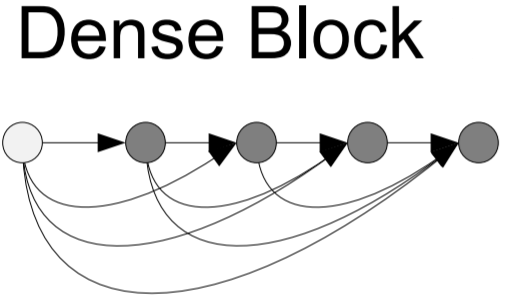
\includegraphics[width=.4\textwidth]{pics/dense block.png}
	\caption{Dense Block}
	\label{fig:dense block}
\end{figure}

\paragraph{Dilated Convolution}空洞卷积。在pooling时,可以减小feature map的尺寸,也能增大每个元素的感受野但是也损失了空间信息。在进行分割时,pooling损失的那部分信息是难以复原的。dilated卷积是一种特殊的卷积,与通常的卷积不同,dilated卷积会在\textbf{卷积核元素之间插入空格},其实相当于一个更大的卷积核,而那些插入的卷积核的值一直为0。如Fig.\ref{fig:dilation}所示。Dilation卷积可以在不做pooling损失信息的情况下增大感受野,pooling虽然可以增大感受野但是失去了位置信息,难以从pooling后的层恢复到原来的信息,而dilation卷积不仅增大了感受野,还保留了特征图中元素的相对空间信息。
\begin{figure}[h]
	\centering
	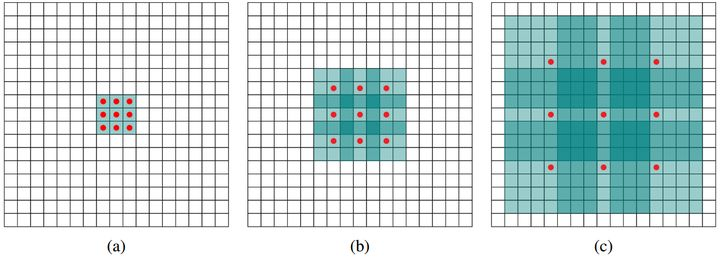
\includegraphics[width=.8\textwidth]{pics/dilation.jpg}
	\caption{Dilation Convolution}
	\label{fig:dilation}
\end{figure}

\paragraph{1 $\times$ 1 Conv}
$1\times 1$卷积很显然,就是卷积核的长宽均为1,用$c_i$ 和$c_o$  分别表示输入和输出通道的数目,为了获得多个通道的输出,可以为每个输出通道创建一个形状为$c_i\times 1 \times 1$ 的卷积核张量,这样卷积核的形状是$c_o \times c_i \times 1 \times 1$。

由于$1\times 1$卷积的长宽为1,无法关注到周围像素的信息,只能关注到同一位置不同通道上的信息,其作用主要由以下几点:
\begin{itemize}
	\item 融合多个通道间的信息
	\item 在不改变feature map尺寸的情况下改变feature map的通道数,例如在图像分割中
	\item 降低参数量
	\item 在以每像素为基础应用时,$1\times 1$卷积相当于全连接层
\end{itemize}
更多解释可参考动手学深度学习:\href{https://zh-v2.d2l.ai/chapter_convolutional-neural-networks/channels.html#times-1}{$1\times 1$  卷积层}

\subsubsection{常用数据增强手段}
增强之前,先想一想:真的需要增强数据吗(通常来说是的)?需要增加的多少数据?需要增加什么样的数据(并不是什么样的数据都可以,主要考虑应用场景中一般会出现的数据即可)?
\paragraph{仿射变换}
仿射变换(Affine Transformation)是指在二维向量空间中进行一次线性变换(乘以一个矩阵)和一次平移(加上一个向量),变换到另一个向量空间的过程。
$$
\left[\begin{array}{l}
	u \\
	v \\
	1
\end{array}\right]=\left[\begin{array}{ccc}
	a_{1} & b_{1} & c_{1} \\
	a_{2} & b_{2} & c_{2} \\
	0 & 0 & 1
\end{array}\right]\left[\begin{array}{l}
	x \\
	y \\
	1
\end{array}\right]
$$

图解,放射变换的种类也如Fig.\ref{fig:affine}所示:
\begin{figure}[h]
	\centering
	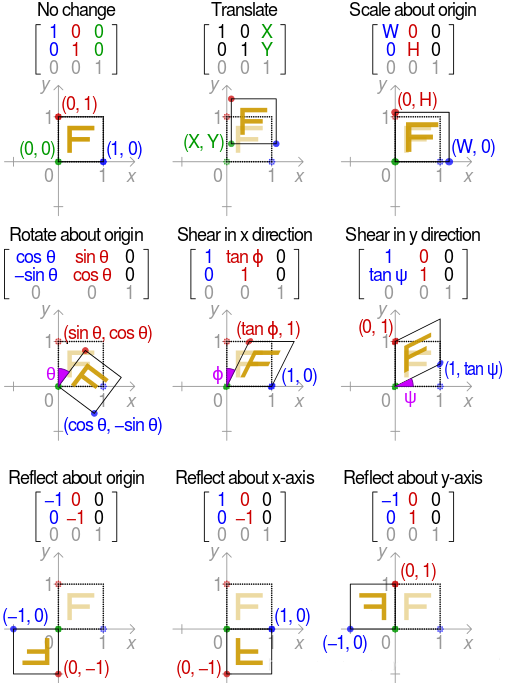
\includegraphics[width=.8\textwidth]{pics/affine.png}
	\label{fig:affine}
	\caption{仿射变换}
\end{figure}

\paragraph{弹性形变\cite{simard2003best}}
最早是从UNet中了解到弹性形变,在细胞分割中,弹性形变发挥了重要作用;弹性形变也用在手写数字识别中。可以发现,在这两种任务中,任务所涉及的对象并不是刚体,简单的仿射变换并不能满足我们的需求。弹性形变所针对的数据特点:对象不是刚体,可能在不同的场景下会有形变。

弹性形变流程:
\begin{itemize}
	\item 对图像imageA进行仿射变换,得到imageB
	\item 对imageB图像中的每个像素点随机生成一个在x和y方向的位移,$\Delta \mathrm{x}$和$\Delta \mathrm{y}$。其位移范围在(-1, 1)之间,得到一个随机位移场(random displacement fields)
	\item 用服从高斯分布的$N(0, \delta)$对step2中生成的随机位移场进行卷积操作(和CNN中的卷积操作一样,说白了就是滤波操作)。我们知道δ越大,产生的图像越平滑。下图是论文中的不同δ值对随机位移场的影响,下图左上角为原图,右上角为$\delta$较小的情况(可以发现,位移方向非常随机),左下角和右下角为较大的不同$\delta$值
	\item 用一个控制因子$\alpha$与随机位移场相乘,用以控制其变形强度
	\item 将随机位移场施加到原图上,具体是\textbf{怎么施加的呢}?首先,生成一个和imageB大小一样的meshgrid网格meshB,网格中的每个值就是像素的坐标,比如说meshgrid网格大小为512x512,则meshgrid中的值为(0, 0), (0, 1), ..., (511, 0), (511, 511),然后将随机位移场和meshB网格相加,这就模拟了imageB中的每个像素点在经过随机位移场的作用后,被偏移的位置,meshB与随机位移场相加后的结果记做imageC
	\item 弹性变形最终输出的imageC中每个位置的灰度值大小,组成一副变形图像,现在imageC中每个像素点存储的是$(\mathrm{x}+\Delta \mathrm{x}, \mathrm{y}+\Delta \mathrm{y})$,如下图中的$\mathrm{A}^{\prime}$,那怎么转化成灰度值呢,依据论文,作者是根据imageB中的B位置的双线性插值灰度值作为$\mathrm{A}^{\prime}$点的像素灰度值大小(如Fig.\ref{fig:elastic-deform}所示),最终将imageC输出得到变形图像
\end{itemize}
\begin{figure}[h]
	\centering
	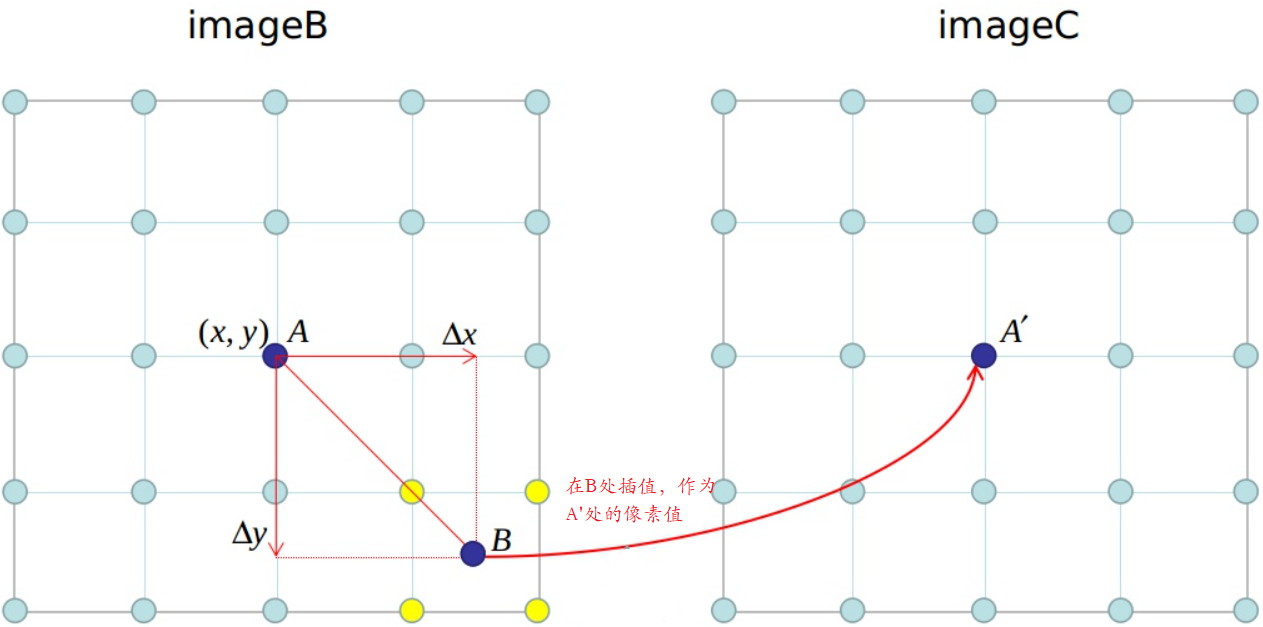
\includegraphics[width=.8\textwidth]{pics/elastic_deform.png}
	\label{fig:elastic-deform}
	\caption{弹性形变}
\end{figure}
参考:\href{https://zhuanlan.zhihu.com/p/342274228}{数据增强:弹性变形(Elastic Distortion)}。

\paragraph{增加噪声}
如椒盐噪声。

\paragraph{GAN}


\subsubsection{方差与偏差}
\paragraph{偏差(Bias)}讲模型的方差的时候,通常是指:对于一个模型,它的预测结果与真实值之间的差距。方差度量的是学习到的函数与真实函数的差距的期望,即$E[\hat{f} - f]$。

\paragraph{方差(Variance)}选用一种模型(如KNN,SVM,NN等),使用不同的数据可以得到该种模型的多个实例(即训练好参数的模型)。\textbf{这些模型}对于同一个输入给出的预测值的方差,即$E[(\hat{f} - E[\hat{f}])^2]$。方差是受所使用的训练集影响的,我们使用不同分布的数据集训练出来的模型会导致学出来的模型参数变化,这反映出来的就是针对同样的输入会产生不一样的预测值,这些预测值的方差就反映了模型的方差。

在模型很复杂的时候,在训练集上学习的模型能够准确地预测,产生较小的偏差,但是更容易产生大方差,因为模型有更多的参数,能够“死记硬背”记下输入与输出的映射关系,这个时候模型可能记住了一些没用的东西甚至是噪声,而模型是没有见过测试集的,稍微有些不同的数据点的输出可能会有较大的差别,从而产生大的偏差。 --- \textbf{过拟合}

当模型较简单的时候,可能无法充分地利用训练集,在测试集上会产生较大的偏差,但是因为模型参数少,模型关注地特征较少,光从这些特征来看的话,测试集中的数据与训练集中的数据会有更高的相似性,因此就算不同的数据输入,但是由于某些特征被忽略后数据反而是相似的,所以模型给出的输出是类似的,因而方差小。--- \textbf{欠拟合}

参考:\href{http://scott.fortmann-roe.com/docs/BiasVariance.html}{Understanding the Bias-Variance Tradeoff}。


\textbf{注意:}\textbf{一种模型相当于一个函数空间},当我们选择一种模型进行训练,得到了该种模型的各个参数,就相当于得到了一个实例化的模型。模型种类相当于类,训练好的模型相当于对象。喂数据训练模型时相当于在某个特定的函数空间中找到一个合适的函数 --- 即我们要的模型。有时候训练后的模型效果不好,可能不是这种模型不行,可能是没有在这个函数空间中找到合适的函数。

\subsubsection{类别不平衡问题}
指的是监督学习中,不同类别的样本数目具有较大的差异(样数据分布与均匀分布差异较大)。
\paragraph{类别不均衡可能造成的问题}
\begin{itemize}
	\item 一些评价指标可能失效。例如在癌症检测中,可能$99\%$的样本都是0,只有$1\%$的样本为1,这个时候即使将所有样本预测为0也能有很好的acc,但是漏检是很严重的!类别不平衡使得一些评价指标并不能反映模型真是的能力
	\item 
\end{itemize}

\paragraph{决解办法}
\subparagraph{数据角度}
中心思想就是直接改变数据分布。
\begin{itemize}
	\item 获取更多数据,使数据分布趋向于均衡
	\item 上采样。通过一些方法,使得占少数的类别(minority类)的样本数增加,常用的方法:
	\begin{itemize}
		\item 重复采样minority类,使其样本数增加
		\item 合成的方法。根据已有数据集生成新的样本,如SMOTE方法及其变体
		\item 基于聚类。分别对major和minority类进行聚类,再通过过采样的方法使得major和majority中各个簇的数量相等,例如原本major类聚类后样本数目比为1:2:3,minority类聚类后为1:2,通过过采样的方法,先使majority与minority样本数相等,再使类内部各个簇的数目相等。这样不仅可以解决类别间的不平衡,还可以解决类内部的不平衡
	\end{itemize}
	\item 下采样。通过一些方法把占多数的类别(major类)的样本数降低。下采样的方法有很多
	\begin{itemize}
		\item 随机下采样,从major类中随机保留一部分样本
		\item 基于临近样本,来选择保留哪些major类样本
		\item 基于聚类,对major类进行聚类,使其具有N(minority类样本数)个簇,用这N个簇的中心作为major类采样后的样本
	\end{itemize}
\end{itemize}

\subparagraph{算法角度}
\begin{itemize}
	\item 选择对数据倾斜相对不敏感的算法,如树模型等
	\item 在下采样时会损失一部分信息,可以从major类中采样多个数据集来学习不同的模型,即集成学习(Ensemble集成算法)。首先从多数类中独立随机抽取出若干子集,将每个子集与少数类数据联合起来训练生成多个基分类器,再加权组成新的分类器,如加法模型、Adaboost、随机森林等
	\item 将任务转换成异常检测问题。譬如有这样一个项目,需要从高压线的航拍图片中,将松动的螺丝/零件判断为待检测站点,即负样本,其他作为正样本,这样来看,数据倾斜是非常严重的,而且在图像质量一般的情况下小物体检测的难度较大,所以不如将其转换为无监督的异常检测算法,不用过多的去考虑将数据转换为平衡问题来解决
\end{itemize}

\subparagraph{评价指标角度}
\begin{itemize}
	\item 混淆矩阵
	\item F-score
\end{itemize}

\subsubsection{交叉验证}
在训练模型的时候,通过会把数据集划分为训练集和测试集,测试集的作用用于学习模型参数,测试集是为了检验模型在未见过的数据上的效果。但是只将数据集划分为测试集和训练集有以下问题:
\begin{itemize}
	\item 最终模型与参数的选取将极大程度依赖于你对训练集和测试集的划分方法。不同的划分情况,学习出来的参数是不一样的;固定模型参数,模型在不同划分上的表现也是不一样的。这种情况使得我们无法准确对模型的能力进行评估,不利于我们选择最优的模型(指何种模型)以及最优的模型参数(一般是指超参数,而不是模型学习到的参数);
	\item 该方法只用了部分数据进行模型的训练,无法充分利用已有的数据。测试的效果只是针对某个划分,并不是针对整个数据集,不够有说服力;
\end{itemize}
为了解决以上为题,即1)选择最好的模型与参数;2)充分利用数据,使模型的测试结果有说服力,就有了交叉验证(Cross Validation)。常见的交叉验证方法:
\begin{itemize}
	\item LOOCV(Leave-one-out cross-validation),即留一验证。对于有N个样本的数据集,重复N次,每次选择其中一个作为测试集,其他的作为训练集,这样就得到了N个$(train_i, test_i), i = 1, ..., N$训练集、测试集对儿。分别用这N个训练集-测试集对儿来训练模型,这样就可以学习到N个模型。每个模型都可以得到一个测试得分,进行平均后就作为这类模型在这个数据集上的测试分数
	
	\item K-fold CV,即K折交叉验证。与LOOCV类似,但是对数据集的划分不同,是把数据集划分为K份,每次取其中一份作为测试其,其余作为训练集,这样就可以得到K个测试得分,进行平均后作为最终的测试分数
\end{itemize}
\textbf{注意:给定模型种类和一组超参数,这样就确定了一个模型,但是模型的参数需要通过数据来学习(如Fig.\ref{fig:model}所示),比如线性回归中的权重,上述的N个或K个模型是针对某个模型种类和一组超参数组合而言,K或N个不同的训练集学习到的K或N个模型,但它们的超参数都是一样的},具体过程就是:\tbc{red}{确定模型类别 ==> 确定超参数 ==> 喂数据进行学习(喂K次不同的数据) ==> 得到K个模型(但是超参数都一样) ==> 计算平均得分 ==> 得到这种模型在这种超参数下的得分},这也就是CV可以用于选择模型(\textbf{选择模型最优的超参数})的原因。

\begin{figure}[h]
	\centering
	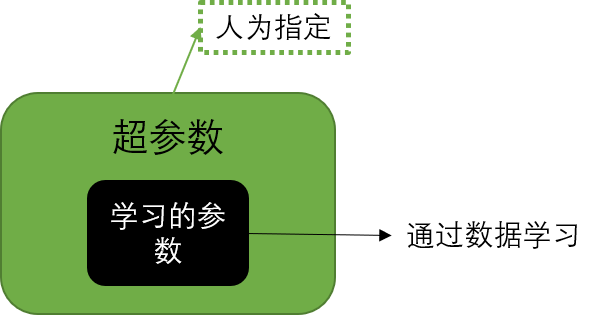
\includegraphics[width=.5\textwidth]{pics/model.png}
	\label{fig:model}
	\caption{模型的超参数与学习参数}
\end{figure}

一些值得注意的问题:
\begin{itemize}
	\item LOOCV计算成本太高而且不同训练集之间的重合度太高
	\item K的选取。K太大,投入的训练集也大,得到的模型可能会有较小的偏差,但是由于训练集之间的重叠度较高,会存在较高的方差
\end{itemize}


\subsubsection{归一化 vs 标准化 定量的分析}
参考:\href{https://mp.weixin.qq.com/s/lO3Li7dWAvtzefVA_M0dJg}{https://mp.weixin.qq.com/s/lO3Li7dWAvtzefVA\_M0dJg}\\
\textbf{归一化:}将值变换到$[0, 1]$或者$[-1, 1]$之间,使得不同类型的特征之间有了可比性,对利用了样本之间距离的算法很重要。\textbf{标准化:}改变数据的统计特征,如将均值和方差变为0和1。在现实中,一个变量极有可能是服从正态分布的。


一些重要的结论:
\begin{itemize}
	\item 对于不同的算法,可能不同的缩放方法有不同的效果,例如Tree-based模型对特征的尺度是不敏感的,而一些依赖样本之间的距离的方法则对尺度很敏感,如KNN
	\item 归一化可能会将数据点挤压到一起
\end{itemize}



\section{NLP}
\subsubsection{马尔科夫链/隐马尔科夫链}
马尔可夫模型主要用于研究时间序列的分布的,若已有一个是时间序列:$X_0, X_1, X_2, ..., X_n$,马尔可夫模型要解决的就是这些随机变量的取值是如何随着时间而变化的、每个随机变量取值的概率 --- 这些随机变量取值的分布。随机变量的取值可以称为状态。那么问题就成了:
$$
P(X_0=s_0, X_1=s_2, ..., X_n=s_m) = ?
$$
或者说,下一个时刻的随机变量的取值问题:
$$
P(X_n | X_0=s_0, X_1=s_2, ..., X_{n-1}=s_{m-1}) = ?
$$
为了简化这个问题,有了马尔科夫假设。

(1阶)马尔可夫假设:当前状态的取值只取决于前一个时刻的状态。即:
$$
P(X_n | X_0=s_0, X_1=s_2, ..., X_{n-1}=s_{m-1}) = P(X_n | X_{n-1}=s_{m-1})
$$
满足这样性质的一系列随机变量串联在一起就是马尔科夫链了。

那隐马尔科夫链与马尔科夫链又有什么关系呢?
隐马尔科夫模型描述的是两个时序序列的联合分布:$p( \boldsymbol{X}, \boldsymbol{Y} )$,其中$\boldsymbol{X}, \boldsymbol{Y}$均为时序序列,通常称$\boldsymbol{X}$为观测序列,$\boldsymbol{Y}$为状态序列 --- 不可观测序列。其中观测序列/状态序列均可视为随机变量序列(注意,同一时刻的观测变量和状态变量并不是独立的),观测变量序列的取值为可观测值,状态变量序列的取值为状态值 --- 与马尔可夫模型中的状态含义一致。隐马尔科夫模型的假设:
\begin{itemize}
	\item 当前状态变量$\boldsymbol{Y}_t$的取值仅以来与前一个状态变量$\boldsymbol{Y}_{t-1}$的取值有关,连续多个状态变量的取值则构成隐马尔科夫链
	\item 任意时刻的观测变量$\boldsymbol{X}_t$取值仅依赖于该时刻的状态变量的取值$\boldsymbol{Y}_t$
\end{itemize}

一个隐马尔科夫模型可以表示为:$\lambda = (\boldsymbol{\pi}, \boldsymbol{A}, \boldsymbol{B})$,含义如下:
\begin{itemize}
	\item $\boldsymbol{\lambda}$:初始状态概率向量,即初始时刻的状态变量$\boldsymbol{Y}_0$取值为各个状态的概率
	\item $\boldsymbol{A}$:状态转移概率矩阵,即上一时刻的状态变量取某值时,当前时刻状态变量取值的概率分布:$p(\boldsymbol{Y}_t=s_j | \boldsymbol{Y}_{t-1}=s_i)$
	\item $\boldsymbol{B}$:发射概率矩阵,即当前状态变量取某值时观测变量取某观测值的概率分布:$p(\boldsymbol{X}_t=o_j | \boldsymbol{Y}_t=s_j)$
\end{itemize}

其实,可以看出马尔可夫模型是隐马尔科夫模型的一个特例 --- 状态变量序列与观测变量序列相同,状态值即为观测值,每个状态只对应一个观测值即本身。

隐马尔可夫模型的三个应用:
\begin{itemize}
	\item 样本生成问题:给定模型$\lambda = (\boldsymbol{\pi}, \boldsymbol{A}, \boldsymbol{B})$,生成满足模型约束的样本 --- 观测序列即对应的状态序列
	\item 模型的训练:给定训练数据 --- 观测序列即对应的状态序列,估计模型参数$\lambda = (\boldsymbol{\pi}, \boldsymbol{A}, \boldsymbol{B})$
	\item 序列预测:已知模型参数$\lambda = (\boldsymbol{\pi}, \boldsymbol{A}, \boldsymbol{B})$,给定观测序列,求状态序列
\end{itemize}

怎么解决上述的三个问题呢?

对于样本生成问题,其实很简单,指要逐步采样状态,得到一个状态序列,在根据每一步的状态取值采样得到观察值,就可以得到观测序列,样本生成就完成了。

对于模型的训练问题,需要估计的参数为:$(\boldsymbol{\pi}, \boldsymbol{A}, \boldsymbol{B})$,对于$\boldsymbol{\lambda}$则统计所有的状态序列中,计算以每个状态为开头的序列的频率即可,其他两个概率矩阵的训练类比即可。

对于序列预测问题可以通过维特比算法解决。给定一个观测序列,求解最有可能的状态序列。本质上这是一个搜索问题,搜索最有可能的状态序列,使观测序列的似然概率最大。简要地说一下。

维特比算法通过动态规划的方法解决这个问题。假设我们已经有最优的状态路劲,那么其中一条从起点开始的子路径也是最优的子路径。因此可以通过维护两个动态规划的矩阵来记录路径的选择和其概率。假设有两个矩阵$\boldsymbol{\sigma}, \boldsymbol{\psi}$。其中$\boldsymbol{\sigma}_{ti}$表示在时刻$t$时以$s_i$结尾的所有局部路径的最大概率,$\boldsymbol{\psi}_{ti}$表示在时刻$t$时末状态为$s_i$的前驱状态。

\paragraph{应用}使用隐马尔科夫模型可以解中文分词问题。给定训练数据 --- 每个样本为一个句子,对于每个样本,目标是给每个词分配一个标签(如{B, M, E, S}),然后可以根据序列对句子进行分词。为达成这个目的,需要训练隐马尔科夫模型,获得模型的各个参数,根据训练数据是否被标注可以使用不同的方法进行训练。获得训练数据后即可使用模型进行序列预测任务,再根据序列进行分词。


\colorbox{red}{注:本节内容主要参考何晗所著《自然语言处理入门》}。


\subsubsection{概率图模型}
将联合概率分布以图的形式来表示,可以分为有向概率图模型和无向概率图模型。
概率图模型中,将随机变量表示为结点,相关联的随机变量之间会有边连接。

有向图模型中按变量的因果关系进行连接,可以刻画变量之间的因果关系。有向图表示的联合概率可以根据图中的变量依赖关系分解成多个条件概率的积。(听着有点像拓扑图)

无向图模型没有体现出因果关系,强调的是变量之间的相互关系。无向图模型将联合概率分布分解为“无向图中-最大团上-随机变量的函数-的乘积”。

\subsubsection{命名实体识别}
NLP中的命名实体识别(Named Entity Recognition)指的是将识别出文本中描述实体的词汇,比如人名、地名、组织机构名、股票基金、医学术语等,更一般地讲,不同的领域会有不同的实体,用于描述该领域内的实体对象。NER的目的就是识别出文本中实体与其他文本的边界和实体的类别。主要以下几个难点:
\begin{itemize}
	\item 实体的数量是无穷的。不同的领域会有不同的实体,且实体并不是定量的,会不断的增加
	\item 实体的构词灵活。同一个实体可能会有多个名字,比如实体的简写;实体也可能是嵌套形成的
	\item 类别模糊。同一个实体在不同的语境下可能会有不同的类别
\end{itemize}

命名实体的识别,从某个角度来看可以视作一个序列标注问题。具体做法是将命名实体附着到{B, M, E, S}标签。其实,词性标注问题也可以以这样的方法来处理。更一般地看,词性标注与命名实体识别是同一个问题,它们都需要对文本进行分词,词性标注中的词性和NER中的实体类别是等价地。

\subsubsection{TF-IDF}
词频-倒排文档频次。通常用于衡量一个词语在文档中的重要程度。单单使用词频评价词语重要程度是不全面的,有些词可能会在文档中出现很多次,但是如果其在很多文档中都出现,却又体现不了其重要性。因此,需要一个对词频进行扩充,希望得到的重要的词应该是这样的:词频高,同时又不是出现在大部分文档中。
$$
TF-IDF(t, d) = \frac{TF(t, d)}{DF(t)} = TF(t, d) \cdot IDF(t)
$$
其中,$TF(t, d)$表示词$t$在文档$d$中出现的次数,$DF(t)$表示包含词$t$的文档数。实际中计算$TF-ID$时会加入一些平滑操作(如加一平滑、对IDF取对数)防止结果下溢等。 IDF表示inverse document-frequency,计算方法:
$$
IDF(t) = \log \frac{1 + n}{1 + DF(t)}
$$
\begin{center}
	或
\end{center}
$$
IDF(t) = \log \frac{n}{1 + DF(t)} + 1
$$
计算得到一个矩阵,每一行表示一个文档的tf-idf向量,每个元素表示对应的词(term)在该文档种的重要程度,一般还会进行$l2$正则化。

\subsubsection{词袋模型}
用于表示文档/句子(其实句子可以看作只有一个句子的文档)的一种方法。
词袋模型一般会先构建一个词表,每个文档经过分词后,可以使用不同的统计量来构建文档/句子的向量,词表之外的词不予考虑。可以选用的不同的统计量有:
\begin{itemize}
	\item 词频
	\item 布尔词频
	\item TF-IDF
	\item 词向量
\end{itemize}

\subsubsection{使用朴素贝叶斯分类器进行文本分类}
首先,给定类别数为$c$,每个文档的特征向量长度为$n$。

朴素贝叶斯分类器是一个生成式的分类器,其计算的是$p(Y | X)$,对于生成模型,重要的是要学习联合分布$p(X, Y)$,朴素贝叶斯通过训练数据学习该联合分布:$p(X, Y) = p(Y)p(X|Y)$。对于给定样本$X^i$,对其进行分类可形式化为:
$$
y = \mathop{argmax}_{c_k} p(Y=c_k | X=X^i) = \mathop{argmax}_{c_k} \frac{p(X=X^i | Y=c_k) p(Y=c_k)}{p(X=X^i)}
$$
朴素贝叶斯中假设样本的特征之间是相互独立的,即$p(X)=p(X_1=x_1, ..., X_n=x_n) = p(X_1=x_1) ... p(X_n=x_n)$。那么为了得到样本$X^i$的类别,只需要计算出$p(X=X^i | Y=c_k),  p(Y=c_k), p(X=X^i)$即可。而对于某一个样本的分类,$p(X^i)$对分类是没有帮助的,在$Y$取不同类别时是不会变化的,故可以不计算$p(X^i)$。那么剩下的需要计算的只有出$p(X=X^i | Y=c_k),  p(Y=c_k)$了。

$p(Y=c_k)$是很好计算的,只需要统计训练数据中类别为$c_k$的样本所占的比例即可。由于特征之间独立的假设,所以$p(X^i | Y=c_k) = \prod_{j=1}^{n} p(X_{j}^{i}=x_j | Y=c_k)$。这个概率也只需要从训练数据中统计即可,统计每个类别下,特征向量的第$j$维取$x_j$的比例即可。

关于样本的特征向量:通常可以采用词袋模型的方法来表示一个文本/句子。

\subsubsection{语法分析}
分析句子中的语法结构并将其表示为容易理解的结构(通常为树形结构)。
\paragraph{短语结构树}根据上下文无关文法将句子/短语分解为树状结构。短语结构语法(上下文无关文法)描述了如何自定向下地生成一个句子,同样句子/短语也可以通过短语结构语法进行分解。这其实和编译原理中的上下文无关文法是很类似的,也是通过很多产生式进行推导,那么是否可以使用编译原理中的词法分析来解决这个问题呢?

\paragraph{依存句法树}关注的是句子中词语之间的语法关联系,并将其约束为树形结构。在句子中,如果一个词语修饰另一个词语,则称修饰词为从属词,被修饰词为支配词,两者之间的语法关系称为依存关系,在可视化时,由支配词指向从属词。依存句法树描述了句子中的各个词之间的依赖关系,一般约定同一个词不能依存于多个词。

\textbf{复合性原理}:一个复杂表达式的意义是由其各组成部分的意义以及结合它们的规则决定的。通过将句子分解为短语、分解短语为单词,下游应用会得到更多更深层次的结构化信息。

\subsubsection{Transformer}
在NLP中有很多输入为序列输出为序列的\textbf{seq2seq}任务,例如机器翻译、文本摘要、序列标注、文本生成等等。早期的seq2seq任务RNN-based\cite{sutskever2014sequence, cho2014learning}模型为主,但RNN-based的模型容易出现以下问问题:
\begin{itemize}
	\item RNN处理seq2seq任务时通常将输入序列转换成一个context向量,再基于context来得到输出的序列。单个向量难以包含输入序列的所有信息
	\item RNN在递归的解码过程使得其难以处理长文本序列
	\item RNN的反向传播容易出现梯度弥散/爆炸问题
	\item 序列的处理是串行的,难以并行化,计算效率低
\end{itemize}
\textbf{Attention}\cite{bahdanau2016neural, luong2015effective}技术 --- 帮助RNN-based模型解决了一部分困难。具体是怎么做的呢?在RNN-based模型的基础上主要有以下几个变化:
\begin{itemize}
	\item 编码器传给解码器的不再只是一个context向量,会利用编码过程中的所有隐向量
	\item 解码时,会根据所处的时间步,为每一个隐向量计算一个分数,归一化后再分别与隐向量相乘得到当前时间步的context向量
\end{itemize}

有了Attention,RNN-based模型的一部分缺点得到了解决(处理长文本序列的问题),但还是有一些问题:不能并行化处理输入序列,且能不能直接在Attention上构建seq2seq模型呢?

\textbf{Transformer}\cite{vaswani2017attention}来了!!!
Transformer采用的也是编解码的结构:先对输入序列进行编码,再根据编码的输出进行解码。与RNN-based模型不同的是,其


\section{Graphs}
% 记录一些常见的图的概念
\subsubsection{图基本概念}
\paragraph{Motif} 形式上是一个连通子图,强调这个Motif的拓扑结构。Motif可能是某种经常出现在图中的结构,可以认为时一种反复出现的结构模式。相同结点数的motif可能会有多种结构。

\paragraph{Weisfeiler-Lehman isomorphism test}  图同构测试。对于两个图$G_1, G_2$,WL test能够判断它们是否同构,但是也存在一些特殊的例子,WL test会将非同构的两个图判定为同构的。算法过程如下:
\begin{enumerate}
	\item 对$G_1, G_2$中的结点都赋予一个标签,都为1;
	\item 对于每个结点$v$重复执行:
	\begin{enumerate}
		\item 汇集$v$的邻居结点的标签,放在一个列表里,$S_v = \{u_l | u \in \mathcal{N}_v \}$
		\item 将$v$的标签$v_l$和S组合成一个pair---$(v_l, S_v)$
	\end{enumerate}
	\item 利用一个hash函数将每个结点的$(v_l, S_v)$映射成一个新的标签,将新的标签赋予给对应的结点。至此一轮迭代就结束了,如果图中结点的标签都没发生变化则结束,否则返回步骤2.
\end{enumerate}
上述过程是针对一个图来说的,可以同时分别对$G_1, G_2$执行上述算法。
当迭代结束后怎么判定两个图是否同构呢?
WL test中是这样做的:\\
分别计算图中每个标签的数量(也就是标签的分布),可能会得到类似这样的一个结果(1: 2, 2:3, ...),这表示标签1出现了2次,标签2出现了3次。如果最后两个图这个结果是一致的,那么不排除它们同构的可能性。

基于WL test 算法,WL subtree kernel\cite{shervashidze2011weisfeiler} 构建以某个结点为根的子树,来代表该结点的特征。

\paragraph{图算法(GNN)中常用的benchmar以及数据集} 常用的图数据集主要可以分为这几类:
\begin{itemize}
	\item 生物信息类的图数据。如MUTAG, PTC, NCI1,PROTEINS 分子,药物的一些图数据
	\item 社交网络。如Facebook, Reddit 等
	\item 引文网络。如 Cora, PubMed, Citeseer等
\end{itemize}

斯坦福大学的SNAP组有很丰富的图网络数据集:\href{http://snap.stanford.edu/data/index.html}{Stanford Large Network Dataset Collection}


\paragraph{Heterogeneous graph, Attributed graph}同构图和属性图,同构图中,有多种类型的结点和边。Attributed graph中结点会有较丰富的属性(个人感觉可以理解为特征)。一个简单的分类:
\begin{table}[h]
	\centering
	\begin{tabular}{|c|c|c|c|}
		\hline
		\rowcolor[HTML]{4371C3} 
		{\color[HTML]{FFFFFF} \textbf{Graph Types}}                            & {\color[HTML]{FFFFFF} \textbf{Homogeneous}} & {\color[HTML]{FFFFFF} \textbf{Multi-Relational}} & {\color[HTML]{FFFFFF} \textbf{Heterogeneous}} \\ \hline
		\rowcolor[HTML]{CED6EA} 
		\textbf{\#of node types}                                               & \textbf{1}                                  & \textbf{1}                                       & \textbf{\textgreater{}1}                      \\ \hline
		\rowcolor[HTML]{E9EBF6} 
		\multicolumn{1}{|l|}{\cellcolor[HTML]{E9EBF6}\textbf{\#of edge types}} & \textbf{1}                                  & \textbf{\textgreater{}1}                         & \textbf{\textgreater{}=1}                     \\ \hline
	\end{tabular}
\end{table}

\paragraph{Graph Kernel}

\paragraph{Dynamic graph, Streaming graph}动态图和流图。动态图主要指在给定的(static)的结点集上,随着时间,边发生变化;而流图则是结点集和边都会随着时间而变化。

除了结点和边的变化,可能结点/边的标签也会发生变化,更具体的,结点/边的属性也会变化。

\paragraph{图的同构}对于两个图$\mathcal{G}_1 = (V_1, G_2), \mathcal{G}_2=(V_2, E_2)$,如果两图之间的结点能够一一对应,令该映射为$f$,

若$\forall v_i^1, v_j^1 \in V_1, v_i^2, v_j^2 \in V_2$,$f(v_i^1) = v_i^2, f(v_j^1) = v_i^2$,当$(v_i^1, v_j^1) \in E_1$有$( f(v_i^2), f(v_j^2) ) \in E_2$,则称$\mathcal{G}_1, \mathcal{G}_2$是同构的,存在同构映射$f$。

\subsubsection{结点邻居采样}
在图机器学习中,生成结点表征可以说是最基本的事儿了。不管是随机游走、矩阵分解还是图神经网络的方式,最终都会得到结点的表征。其中不可绕过的一个就是结点的邻居。
在随机游走中,会类似于语言模型中词语的上下文环境一样为结点构造上下文,每个结点产生的随机游走路径就是一个上下文。游走的过程可以看作是对结点邻居进行采样的过程。矩阵分解中,通常是构造图的Laplacian矩阵,再进行分解,用特征向量来表示结点表征,对这个不是很了解,就不多说了。到了图神经网络中,节点邻居更是成了主角。从GCN原论文\cite{kipf2017semi-supervised} ==> GraphSage\cite{hamilton2017inductive} ==> FastGCN\cite{chen2018fastgcn} ==> VR-GCN\cite{chen2018stochastic} ==> ... 。GCN中结点的邻居采样方式五花八门。

\begin{enumerate}
	\item GCN原论文中,再进行图卷积时需要把整个graph全部加载进内存,为了求一个结点的表征需要对整个graph进行卷积
	\item GraphSage中,并不使用结点的所有邻居,而是对每个结点的邻居进行采样,得到固定数目的采样后的邻居
	\item FastGCN中引入了importance sampling
	\item 审稿时发现的根据attention distribution 和 uniform distribution的KL散度选top-k的采样。这种方法可以发现比较重要的结点,而不是均匀地参与到其邻居的结点
\end{enumerate}

\subsubsection{DeepWalk \& Node2Vec}
二者都是学习结点表征的方法,都是通过游走的方式来生成一个节点的context,在通过SkipGram的方式来学习结点表征。二者关键的差别就在生成context的方式,即游走方式上。

\begin{itemize}
	\item DeepWalk不适用于有权图,不能学习权重对graph、结点带来的影响;Node2Vec能够处理带权图
	\item DeepWalk中使用的是RandomWalk。给定一个结点$v$,下一步访问的结点通过均匀采样$v$的邻居结点来得到
	\item Node2Vec中用了两个参数来控制游走,即如何采样下一个结点
\end{itemize}
重点介绍以下Node2Vec中的randomwalk,如Fig.\ref{fig:node2vec}所示。
\begin{figure}[h]
	\centering
	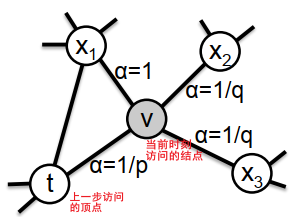
\includegraphics[width=.5\textwidth]{pics/node2vec.png}
	\label{fig:node2vec}
	\caption{Node2Vec中的随机游走}
\end{figure}
Node2vec中的随机游走是二阶的随机游走,为什么叫二阶的呢?在Deepwalk中,随机游走只与当前时刻访问的结点有关,直接从当前节点的邻居中进行均匀采样,这叫一阶。Node2vec中的二阶是指:当前访问的结点$v$,下一步访问的某个节点概率将由上一时刻访问的结点$t$和$v$与邻居的边的权重决定,这是一个二阶马尔科夫链。
$$
P(c_{i}=x \mid c_{i-1}=v)=\left\{\begin{array}{ll}
	\frac{\pi_{v x}}{Z} & \text { if }(v, x) \in E \\
	0 & \text { otherwise }
\end{array}\right.
$$
其中$P(c_{i}=x \mid c_{i-1}=v)$表示当前时刻访问$v$,下一时刻访问$x$的概率,$Z$用于归一化,$\pi_{vx} = \alpha_{pq}(t,x) \cdot w_{vx}$,$\alpha_{pq}(t, x)$为:
$$
\alpha_{p q}(t, x)=\left\{\begin{array}{ll}
	\frac{1}{p} & \text { if } d_{t x}=0 \\
	1 & \text { if } d_{t x}=1 \\
	\frac{1}{q} & \text { if } d_{t x}=2
\end{array}\right.
$$
可见$\alpha_{pq}(t, x)$是一个由$p, q$参数化的函数,函数的自由变量是$t, x$即上一时刻访问的结点和下一时刻访问的结点,其中$d_{tx} \in \{0, 1, 2\}$表示$t, x$间的最短距离。

$p, q$就是控制游走的两个参数:
\begin{itemize}
	\item Return Parameter,$p$,该参数控制下一时刻访问$t$的可能性,如Fig.\ref{fig:node2vec}所示,$p$越小,越有可能访问上一时刻已经访问过的结点$t$,当然还要考虑$w_{vt}$
	\item In-Out Parameter,$q$,该参数能够控制是BFS还是DFS。当$q>1$时,在$p$不变的情况下,访问$d_{tx} = 1$的结点的概率会增大,这就是BFS,当$q<1$时,则会增大访问$d_{tx} = 2$的结点的概率会增大,这就是DFS
\end{itemize}
\begin{figure}[h]
	\centering
	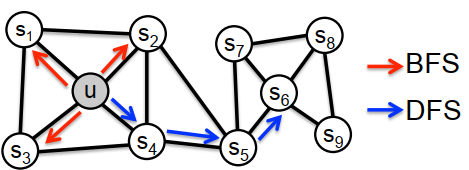
\includegraphics[width=.8\textwidth]{pics/node2vec2.png}
	\label{fig:node2vec2}
	\caption{Homophily与Structure Equivalence}
\end{figure}

论文中将这叫做Biased random walk,通过调整游走的参数$p,q$能够使学习到的表征在同质性(Homophily)和结构相似性(Structure Equivalence)间平衡。BFS能够探索探索homophily,即距离相近的结点,如Fig.\ref{fig:node2vec2}所示,$s_1, s_2, s_3, s_4$是与$u$相邻的结点,它们的表征应该相似;DFS使得探索到更远的地方,能够发现与$u$结构类似地结点,如$s_6$,它俩地表征也应该相似。所以学习到的表征既能体现结点地同质性,也能体现结点地结构相似性。

\section{Knowledge Graph}
\subsubsection{KG中的文本信息抽取}
从纯文本数据中获取有价值的数据,组织成结构化的形式或半结构化的形式。主要包含这几个过程:实体识别、实体消歧、关系抽取及事件抽取。
\paragraph{实体识别}从文本中识别出实体信息。

\paragraph{实体消歧}消除指定实体的歧义。可以分为两类:
\begin{itemize}
	\item 实体链接:将给定文本中的实体指称项链接到已有知识图谱中的某个实体上
	\item 实体聚类:假设已有知识图谱中并没有已经确定的实体,在一个给定一个语料库的基础上,通过聚类的方法消除语料中所有同一实体指称项的歧义,具有相同所指的实体指称项应被聚为一类
\end{itemize}

\paragraph{关系抽取}获取两个实体之间的语义关系。

\paragraph{事件抽取}从描述事件信息的文本中抽取出用户感兴趣的事件信息并以结构化的
形式呈现。
\tbc{red}{kg中的事件能否看作一个subgraph?}


\section{Recommender System}
\subsection{基本概念}

\subsubsection{历史背景}
\paragraph{Motivation}互联网的发展,人们接受的信息越来越多,从信息稀缺时代逐渐过渡到了信息爆炸时代。面对数据的海洋,我们越来越希望我们感兴趣的信息能够直接呈现在我们面前。\tbc{red}{把用户想要的信息推荐给用户} --- 推荐系统的宗旨。

\paragraph{发展过程}:
\begin{itemize}
	\item 1994年,明尼苏达大学GroupLens研究组推出第一个自动化推荐系统GroupLens,提出将协同过滤作为推荐系统的重要技术
	\item 1995年,卡耐基梅隆大学的Robert Armstrong等人提出个性化导航系统Web Watcher;斯坦福大学的Marko Balabanovic等人退出了个性化推荐系统LIRA
	\item 1997年,Resnick等人首次提出Recommender System一词
 	\item 1998年,Amazon上线了基于物品的协同过滤算法,并在千万级用户和百万计商品的规模上进行了应用。Amazon于2003年发表论文\cite{linden2003amazon.com}公布了基于物品的协同过滤算法
	\item 2001年,IBM在其电子商务平台Websphere中增加个性化功能
	\item 2003年,Google开创AdWords盈利模式,通过用户的广告词来提供相关的广告。2007年Google为AdWords添加个性化元素,通过对用户一段时间内的搜索历史进行记录和分析,以便更精准呈现广告
	\item 2006年,Netflix宣布一项竞赛,任何人只要能将其现有的电影推荐算法Cinematch的预测准确度提高10\%就能获得100万美金
	\item 2007年,Yahoo提出SmartAds广告方案,通过分析用户信息以及用户搜索、浏览行为为用户呈现个性化广告
	\item 2007年,第一届ACM推荐系统大会举行
	\item 2015年,Facebook在其官网公布了其推荐系统原理、性能及使用情况(\href{https://engineering.fb.com/2015/06/02/core-data/recommending-items-to-more-than-a-billion-people/}{Recommending items to more than a billion people}),相关论文\cite{he2014practical}
	\item 2016年,YouTube发表论文\cite{covington2016deep}介绍Youtube如何向用户推荐个性化的视频
	\item 2016年。,Google发表论文\cite{cheng2016wide}介绍App商店中的推荐系统,即Wide\&Deep 模型
\end{itemize}

形式上来看,推荐系统的任务是这样的:给定一个输入,从数据集中搜索出一系列数据对象,并排序后输出。

输入通常是关于某个用户的表示,可以是该用户的特征、向量化的表征等,除此之外用户的行为数据,如用户的浏览记录、搜索记录、与商品的交互数据、用户的一些动态变化的数据等都可以与用户特征一起作为输入,而待搜索的数据集中通常是商品的数据,如商品的特征等,基于以上丰富的信息,将输入的信息与数据集中对象进行匹配,给出推荐的顺序。

乍一看,这和搜索很像。其实这么说也没错,都是一个\tbc{red}{Learning To Rank}的任务。其实很多领域研究的问题都很相似,通过进一步的抽象可以看作是同一个问题。但随着研究的深入,为了在一个问题上取得更好的效果,会相应地结合该领域地特点,如领域内特有的信息、领域内特有的数据形式等。因此,虽然问题之间有重叠,但为了做得更好,除了基础的方法,还需要更深入地挖掘领域地特点!例如,在推荐系统中,用户的需求和兴趣是隐含的(隐含在历史数据中,可能用户都不知道自己喜欢什么),而搜索中搜索语句是显式的(用户需求是明确的)。

\paragraph{推荐系统主要元素}
\begin{itemize}
	\item 物品集合:被推荐的物品或内容
	\item 用户:用户的基本信息,如基本信息、行为信息、兴趣爱好等
	\item 场景:用户所处的环境,如网络环境、所处位置等
	\item 推荐引擎:根据用户对物品的偏好与用户的画像数据进行拟合,学习什么样的用户会喜欢什么样的物品。引擎包含以下重要模块:
	\begin{itemize}
		\item 召回模块:根据用户和场景特征,从整个物品数据集(上百万物品)中挑选用户可能感兴趣的物品,\textbf{挑选出一个较小的候选集}(几百至几千)。召回模块中,通常使用简单的特征进行快速查询,比如用户最近点击的物品的相似物品、根据用户兴趣召回物品等。常用的算法:Word2vec、LDA、LSTM、ItemCF、UserCF、DNN等
		\item 排序模块:针对召回模块找到的\textbf{候选集进行精排},得到用户对候选物品集的评分。常用的算法:LR、FM、XGBoost、GBDT+LR、Wide\&Deep、FNN、PNN、DeepFM、NFM、DIN等
		\item 后排模块:得到用户对候选集的评分后,可以根据一些规则对排序进行调整,如运营干预、优先级调权等
	\end{itemize}
	\item 推荐结果集:推荐结果,或推荐结果的有序排列
\end{itemize}

\subsubsection{共现矩阵}
显然,共现矩阵是一种矩阵,\textbf{关键是它描述了一种什么事实}?$M, N(|M| = m, |N| = 2)$表示两个相同或者不同的集合,共现矩阵可以用于表达两个集合笛卡尔乘积的元素对的某种关系,$(m_i, n_j)$间的这种关系可以用共现矩阵的元素$CM_{ij}$表示。

在具体的应用场景中,
\begin{itemize}
	\item 推荐系统:$M$表示用户集,$N$表示商品集,$CM_{ij}$表示用户$m_i$对$n_j$的喜爱程度(如评分)、是否点赞、是否分享等
	\item 自然语言处理:$M = N$表示词汇表,$CM_{ij}$表示词$m_i$与词$m_j$出现在同一个句子中的次数
	\item 社交网络:$M=N$表示作者集合,$CM_{ij}$表示$m_i$与$m_j$间存在某种关系,如朋友关系、合作关系等
\end{itemize}
共现矩阵是两个集合的元素间关系的一个很直白的表达。正是因为直白,共现矩阵通常很稀疏,空间需求大。

\subsubsection{召回方法分类}
召回即从海量的数据集中找出尽可能包含真实结果的候选集。常见的分类:
\begin{itemize}
	\item 行为相似召回:通过用户与物品的交互行为,发现行为指向的物品的相似物品
	\item 相似用户召回:通过用户画像和用户行为等,计算用户之间的相似性,根据相似用户的行为进行召回物品
	\item 内容相似召回:通过对物品内容进行分析,得到物品之间的相似性,根据与用户产生交互的物品来召回
\end{itemize}


\subsubsection{常用相似度计算方法}
\paragraph{同现相似度}
物品A和物品B的同现相似度:
$$
w_{A,B} = \frac{|N(A) \cap N(B)|}{|N(A)|}
$$
其中,$A(A), N(B)$分别表示喜欢A和B的用户集合。但是这种相似度有个问题,当B是热门物品时,喜欢A的用户中可能绝大部分也会喜欢B,那么$w_{A,B}$就会接近于1,即任何物品与热门物品的相似度都会接近于1。除此之外,还有个问题,这个相似度不是对称的,即$w_{A,B} \neg w_{B,A}$,这看起来是有点不合理的,因此,其改进如下:
$$
w_{A,B} = \frac{|N(A) \cap N(B)|}{\sqrt{|N(A)| \cdot |N(B)|}}
$$

\paragraph{欧几里得距离}
众所周知,欧氏距离是欧氏空间中两点之间的距离。两个物品A,B的向量表示为$\boldsymbol{V}_A, \boldsymbol{V}_B$,则欧式距离为:
$$
d(A, B) = ||\boldsymbol{V}_A - \boldsymbol{V}_B||_2
$$
以欧式距离计算A,B间相似性时可如下计算:
$$
sim(A, B) = \frac{1}{1 + d(A, B)}
$$
或许还有其他的形式,例如:
$$
sim(A, B) = e^{-d(A, B)}
$$

\paragraph{皮尔逊相关系数}
介于-1和1之间,它度量两个序列(可以是用户对物品的偏好/评分序列)之间的线性相关程度。它度量数字一起按比例改变的倾向性,也就是说两个数列中的数字存在一个大致的线性关系。当该倾向性强时,相关值趋于1。当相关性很弱时,相关值趋于0。在负相关的情况下一个序列的值很高而另一个序列的值低---相关趋势趋于-1。

使用皮尔逊相关系数计算用户/物品相似度时,通常取共现矩阵中的行(用户对各个物品的偏好)或列(各个用户对一个物品的偏好)作为数列来计算皮尔逊相关系数。两个物品/用户A,B的向量表示为$\boldsymbol{x}, \boldsymbol{y}$,则皮尔逊相关系数为:
$$
r_{\boldsymbol{xy}} = \frac{\sum_i (x_i - \bar{x})(y_i - \bar{y})}{\sqrt{\sum_i (x_i - \bar{x})^2} \sqrt{\sum_i (y_i - \bar{y})^2}}
$$
其实,仔细一看,皮尔逊相关系数和余弦相似度很像,对$\boldsymbol{x}, \boldsymbol{y}$进行标准化后再进行余弦相似度计算。皮尔逊相关系数用于计算相似性时有以下问题:
\begin{itemize}
	\item 没有考虑序列的长短。例如两个用户交互的物品的交集可能会比较大或较小,通常交集较大的情况下更可靠,但是交集更小时计算出的皮尔逊系数可能会更大
	\item 若序列长度为1时,根据定义则无法计算皮尔逊系数
	\item 若序列中的值都相同时也无法计算皮尔逊系数,因为方差为0
\end{itemize}


\paragraph{余弦相似度}
两个物品/用户A,B的向量表示为$\boldsymbol{V}_A, \boldsymbol{V}_B$,则余弦相似度为:
$$
sim(A, B) = \frac{\boldsymbol{V}_A \cdot \boldsymbol{V}_B}{||\boldsymbol{V}_A||_2 \times ||\boldsymbol{V}_B||_2}
$$

\paragraph{Jaccard系数}
两个物品/用户A,B的向量表示为$\boldsymbol{V}_A, \boldsymbol{V}_B$,则Jaccard相似度为:
$$
sim(A, B) = \frac{\boldsymbol{V}_A \cdot \boldsymbol{V}_B}{||\boldsymbol{V}_A||_2 + ||\boldsymbol{V}_B||_2 - \boldsymbol{V}_A \cdot \boldsymbol{V}_B}
$$

\subsubsection{基于人口统计学的推荐}
特征相似的人喜欢的东西应该也类似。根据\textbf{用户画像}(以用户的基本信息作为相似度计算的基础),找出与目标用户相似的用户,将相似用户喜欢的物品推荐给目标用户。这种方法需要构建用户画像。
\paragraph{优点}
\begin{itemize}
	\item 不涉及当前用户的历史喜好,所以解决了“\textbf{用户冷启动}”问题
	\item 不依赖于物品本身的数据,故而无论这个物品是“书籍”、“音乐”还是“短视频”都可以使用,即它是领域独立的
\end{itemize}

\paragraph{缺点}
\begin{itemize}
	\item 用户画像所需要的有些数据难以获取
	\item 以人口统计信息计算相似用户不可靠。特别是“书籍”“音乐”这种涉及到个人喜好的商品,单用这种方法更是难以达到很好的效果
\end{itemize}

\subsubsection{基于内容的推荐}
把用户可能喜欢的物品类型进行推荐,即要找到相似的物品。需要构建物品的特征,如对物品进行标签化。
\paragraph{优点}
\begin{itemize}
	\item 不存在稀疏性和“\textbf{项目冷启动}”问题
	\item 简单有效,推荐结果具有可解释性,不需要领域知识
	\item 基于物品本身特征推荐,不存在过度推荐热门的问题
	\item \textbf{解决了基于人口统计学对个人兴趣建模的缺失},能够很好的建模用户的喜好,实现更精确的推荐
\end{itemize}

\paragraph{缺点}
\begin{itemize}
	\item 推荐的结果\textbf{没有新颖性}
	\item 由于需要基于用户的兴趣偏好进行推荐,故而存在“\textbf{用户冷启动}”问题
	\item 该方法受推荐对象特征提取能力的限制。由于是根据物品相似度进行推荐,故而,物品特征构建模型的完善和全面决定了最后推荐的质量,然而像图像、音频等这种类型的特征难以提取
\end{itemize}

\subsubsection{基于协同过滤的推荐}
Collaborative Filtering,通过群体的行为来寻找相似性(用户或物品的相似性),通过该相似性来做推荐。协同过滤算法可以分为以下几类:
\paragraph{基于用户的协同过滤}
User-based CF(UserCF),根据用户对物品的偏好,发现与当前用户口味和偏好相似的“邻居”用户群,并推荐近邻所偏好的物品。与基于人口统计学的推荐的联系与区别:
\begin{itemize}
	\item 都是基于相似用户来推荐
	\item 不同之处在于如何计算用户相似度:基于人口统计学只考虑用户本身的特征,而UserCF是在用户的历史偏好的数据上计算用户的相似度,它的基本假设是,喜欢类似物品的用户可能有相同或者相似的偏好
\end{itemize}
特点:
\begin{itemize}
	\item 适用于用户数较小的场景
	\item 适用于时效性较强(即物品变化频繁),用户个性化兴趣不太明显的领域,如新闻推荐
	\item 在新用户对很少的物品产生行为后,不能立即对它进行个性化推荐,因为用户相似度表示每隔一段时间离线计算的,故而存在“用户冷启动”问题
	\item 新物品上线后一段时间,一旦有用户对物品产生行为,就可以将新物品推荐给和对它产生行为的用户兴趣相似的其他用户,故而解决了“项目冷启动”问题
	\item 解释性较差,因为计算得到的相似用户可能并不是真的相似,并不能真的反映用户的兴趣。;例如,用户都买了卫生纸、水杯等日常用品并不能表示用户之间相似,但如果都买了键盘、屏幕等,则能较可靠的推断用户是相似的,因此在计算用户相似度时要注意这种大家都会关注的“热门物品”,大家都选择热门物品并不能体现用户的真实兴趣(可以依据社交网络来防止相似用户并不相似)
\end{itemize}

\paragraph{基于物品的协同过滤}
Item-based CF(ItemCF),基于用户对物品的偏好,发现物品和物品之间的相似度,然后根据用户的历史偏好信息,将类似的物品推荐给用户。与基于内容的推荐的联系与区别:
\begin{itemize}
	\item 都是基于相似物品进行推荐
	\item 不同之处在于如何计算物品相似度:ItemCF是根据用户历史的偏好(如共现矩阵)推断,而基于内容的推荐是基于物品本身的属性特征
\end{itemize}
特点:
\begin{itemize}
	\item 适用于物品数明显小于用户数的场合,如果物品很多,计算物品的相似度矩阵的代价就会很大
	\item 适合于长尾物品丰富,用户个性化需求强烈的领域,如电商网站
	\item 用户有新行为,一定会导致推荐结果的实时变化
	\item 新用户只要对一个物品产生行为,就可以给它推荐和该物品相关的其它物品,故而解决了“用户冷启动”问题
	\item 不能在不离线更新物品相似度的情况下将新的物品推荐给用户,故而存在“项目冷启动”问题
	\item 有较强的解释性,因为是依据用户历史偏好的物品来推荐
\end{itemize}


\paragraph{基于模型的协同过滤}
Model-based CF(ModelCF)。基本思想:用户具有一定的特征,决定着他的偏好选择;物品具有一定的特征,影响着用户需是否选择它;用户之所以选择某一个商品,是因为用户特征与物品特征相互匹配。ModelCF基于样本的用户偏好信息,训练一个推荐模型,然后根据实时的用户喜好的信息进行预测,计算推荐。

参考:\href{https://www.cnblogs.com/shengyang17/p/11516532.html}{基于协同过滤的推荐算法}、\href{https://zhuanlan.zhihu.com/p/108759393}{推荐系统——经典算法(基于内容、协同过滤、混合等)}。

\subsubsection{推荐中要注意的点}
\begin{myitemize}
	\item 长尾效应:位于长尾位置的曝光率低的项目产生的利润不低于只销售曝光率高的项目的利润。注意对长尾物品的推荐效果,热门物品的推荐较长尾物品更容易,在评价算法效果时要注意对长尾物品的推荐效果
	\item 用户经常购买的物品并不一定能体现用户的偏好,如很多人都会经常买卫生纸,但这并不能体现用户很喜欢卫生纸,卫生纸作为热门物品反而并不能体现用户的偏好。不同的物品对用户的偏好的贡献是不一样的 --- \textbf{user-aware}
	\item 使用用户行为数据来预测某个用户对某个物品的评分时,要注意历史行为中的物品起的作用可能是不同的\cite{he2018nais}。如预测我会不会买iphone时,可能与我过去买的是什么手机有关 --- \textbf{target item-aware}
	\item 如何对待用户没有交互过的物品?
\end{myitemize}

\subsubsection{常用指标}
此处介绍的指标不涉及具体的计算公式,在不同的场景下有不同的具体定义,计算自然也相应而变。
\paragraph{覆盖率}覆盖率用来描述一个推荐系统对长尾内容或商品的发掘能力。关于覆盖率的定义,最简单的理解是推荐系统能够推荐出来的物品,占平台中全部物品的比例。

\paragraph{多样性}用户的兴趣是非常广泛的,在一个视频应用中,用户可能既喜欢看烧脑电影,也喜欢看动作大片。那么,为了满足用户广泛的兴趣,推荐列表需要能够覆盖用户不同的兴趣领域,即推荐结果需要具有多样性。想提升推荐系统的多样性,就需要在较大的时间跨度上去识别和理解用户的兴趣。

\paragraph{新颖性}新颖,指给用户推荐那些他们以前没有听说过的内容或商品,例如在视频应用中应该尽可能多地向用户推荐他们没有看过的电影。而考虑到很多用户在某个应用中的使用粘性可能并不高,例如一个用户可能同时是多个视频应用的用户,所以仅仅依靠用户在自己系统中的行为记录来保证推荐的新颖性是不够的。

除此之外比较简单方法是基于内容或商品的平均流行度去进行推荐,因为越不热门的东西越可能让用户觉得新颖。

不过,向用户推荐不流行的内容或商品,其实是牺牲了一定的推荐精度的,所以我们需要权衡该指标与其它指标之间的平衡——这不仅在于技术层面的考量,可能也在于商业层面的考量。

\paragraph{惊喜度}如果推荐结果和用户的历史兴趣不相似,但却能够让用户觉得满意,那么就可以说推荐结果的惊喜度很高。想要兼顾推荐系统的惊喜度并不是一件容易的事情,因为这意味着需要降低推荐结果和用户历史兴趣的相似度,所以可能会对预测准确度带来一定的挑战。

但毫无疑问,用户需要惊喜,这会极大提升用户的满意度和使用体验,所以推荐系统对惊喜度的追求只会不断提高,且还需要在不影响预测准确度的前提下来实现。过于关注准确率会导致推荐结果的惊喜度不高。


\subsection{经典算法}
\subsubsection{FM}
Factorization Machine,因子分解机。

\subsubsection{FFM}
Field-aware Factorization Machine,

\section{Learning to Rank}
\subsection{排序学习算法简介}
排序学习,Learning to Rank,简言之:给定一个查询$q$,和待查询的数据集合$D$,返回与$q$最相关的top k(有序)的结果或者给出$D$中所有元素与$q$的相关性排序。

\subsubsection{Pointwise}
将排序问题转化为分类、回归问题。以一个$q$和一个待查询对象$q$(只有一个待查询对象,这也是Point的原因)之间的相关性作为预测目标,即$Pointwise: q \times d \rightarrow label, q \in Q, d \in D$,以$(q, d)$作为训练样本。

Pointwise缺点:
\begin{itemize}
	\item 只考虑了某个查询下,单个待查询对象的相关性,没有考虑该查询下所有待查询对象的排序关系,即带查询对象间的关系
	\item 查询时,往往排在前面的对象比后面的对象更重要,而Pointwise平等地对待所有带查询对象,损失函数会被占多数的非top K对象所影响
\end{itemize}


\subsubsection{Pairwise}
针对一个查询$q$,通过某种方法确定一个大致的待查询对象集合$D_q$,Pairwise将排序问题转化为$D_q$中任意两个对象之间相对关系的分类/回归问题,训练样本为$(d_i, d_j),\: d_i, d_j \in D_q$,预测目标为$d_i, d_j$与$q$的相关性的相对大小,例如1表示$q_i$比$q_j$更相关。

Pairwise缺点:
\begin{itemize}
	\item 是在两个带查询对象之间的相关性的基础上学习的,学习的它们的相对顺序,并不是文档在最终的结果列表中的顺序
	\item 不同的查询可能会有不同大小的带查询对象集合,这种不均衡问题会影响算法的评估与学习
\end{itemize}


\subsubsection{Listwise}
Listwise将一个query对应的所有相关待查询对象看作一个整体,作为单个训练样本,直接优化MAP、NDCG(Normalized Discounted Cumulative Gain)这样的指标,从而学习到最佳排序结果。

\section{Concepts about Math}
\subsection{chap01}
% 记录阅读文献时遇到的一些数学概念等
\subsection{采样}
采样是生成一堆数据的过程,如果最终生成的数据服从某个分布,则可以称这堆数据采样自这个分布。
\subsubsection{alias sampling }
一种高效的针对\textbf{离散概率分布}采样方法,但是要先经过预处理,预处理的时间为$O(n)$,但是与处理完成后采样的时间时$O(1)$。预处理的大致思路如下:\\
对于一个给定的离散概率分布:$p(X = x_i) , X = x_1, x_2, ..., x_n$。按照序号构造n个盒子,每个盒子按照顺序一一与$x_1, ..., x_n$对应,每个盒子的高度为$n \cdot p(X = x_i)$。接下来通过取长补短,把高度高于1的盒子切一部分分到其他高度低于1的盒子上,而且每个序号对应处不能有超过两个盒子。所以需要两个数组(Alias,Accept)来记录预处理的结果,一个用来记录每个序号除了原来的盒子还放了哪个盒子,一个用来记录每个序号的外来盒子有多高。\\
进行采样时,先决定使用哪个序号对应的盒子,再决定使用该序号内的原来的盒子还是外来的盒子。一个简单的例子Fig.\ref{fig:alias-sample}
\begin{figure}[h]
	\centering
	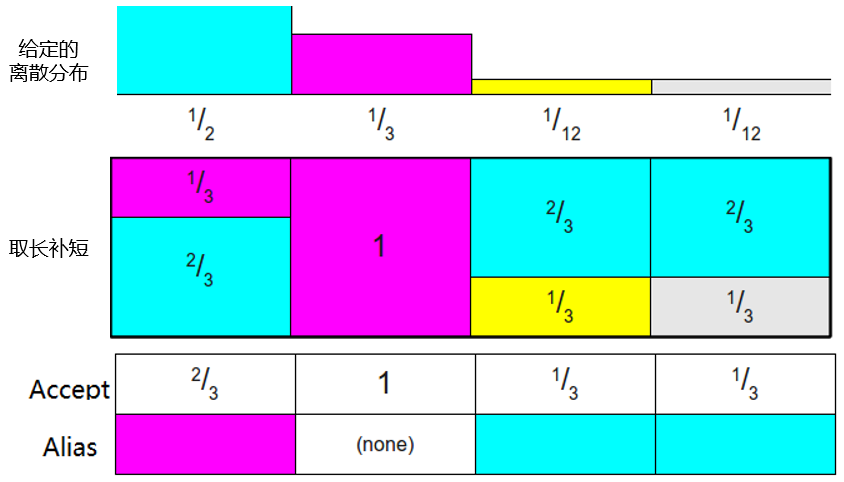
\includegraphics[width=.8\textwidth]{pics/alias-sample.png}
	\label{fig:alias-sample}
	\caption{Alias Sample例子}
\end{figure}


参考资料:
\begin{enumerate}
    \item \href{https://www.keithschwarz.com/darts-dice-coins/}{Darts, Dice, and Coins: Sampling from a Discrete Distribution}
    \item \href{https://www.cnblogs.com/dogecheng/p/13198198.html}{【图嵌入】DeepWalk 和 Node2Vec}
\end{enumerate}

\subsubsection{Importance Sampling}
重要性采样,一种近似的抽样方法, 通过一些数学上的变化, 使得可以对一些不好抽样的分布进行抽样和估计。这个会在强化学习中的off-policy的方法中用到, 从一个策略进行抽样, 更新另外一个策略。求函数$f(x)$的积分可以写成求期望的形式:
$$
E_{x \sim p(x)}[f(x)] = \int p(x) f(x) d x \approx \frac{1}{n} \sum_{i} f(x_{i})
$$
然而通常数据分布会比较复杂且积分也是一个复杂的过程,因此会用采样来代替之。上式中的第三项就是用采样来代替积分,其中$\frac{1}{n}$表示$p(x) = \frac{1}{n}$,即数据的分布。但是有时候$p(x)$是个很复杂的分布,从其重采样是很困难的,这个时候该怎么办呢?

找一个已易于采样的分布$q(x)$,如正态分布,从$q(x)$中采样得到的很多样本作为从$p(x)$中采样的样本集,那么问题就来了,这俩又不是同一个分布,$q(x)$中采样的样本集分布符合$p(x)$吗?先看一个公式:
$$
E_{x \sim p(x)}[f(x)] = \int q(x) \frac{p(x)}{q(x)} f(x) d x \approx \frac{1}{n} \sum_{i}  \frac{p(x)}{q(x)} f(x_{i})
$$
这个就是当我们从$q(x)$中采样代替$p(x)$后求$f(x)$积分/期望的公式。可以看出对于从$q(x)$中采样的样本赋予了不同的权重,因为样本集来自$p(x)$的概率是不一样的,其中重要性就是$\frac{p(x)}{q(x)}$。如Fig.\ref{fig:importance-sample}所示。注意:图中$p(z)$与$f(z)$的含义,$p(z)$是一种分布,是相对于$z$轴的采样点而言的,比如在红色的两个驼峰处,$z$的取点比较多,在其他地方$z$的取点就比较少,这叫样本分布服从$p(z)$。对于$f(z)$是一种映射关系,将$z$值映射到其他维度。

\begin{figure}[h]
	\centering
	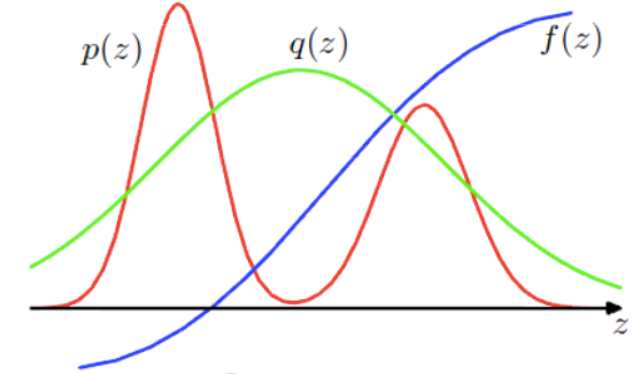
\includegraphics[width=.5\textwidth]{pics/importance-sample.png}
	\label{fig:importance-sample}
	\caption{重要性采样}
\end{figure}

参考:\href{https://www.jianshu.com/p/3d30070932a8}{随机模拟-Monte Carlo积分及采样(详述直接采样、接受-拒绝采样、重要性采样)}。


\subsubsection{接受-拒绝采样}
同样的问题:对于一个难以采样的分布$p(x)$,该怎么采样呢?选择一个易于采样的分布$q(x)$,从中采样,以一定的概率接受或拒绝采样到的样本,使得经过筛选后的样本集是服从$p(x)$的。
\begin{figure}[h]
	\centering
	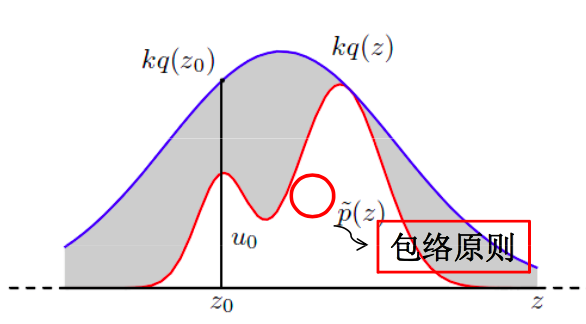
\includegraphics[width=.6\textwidth]{pics/accept-reject-sample.png}
	\label{fig:accept-reject-sample}
	\caption{接受-拒绝采样}
\end{figure}
具体该怎么操作呢?如Fig.\ref{fig:accept-reject-sample}所示,选择$q(x)$,乘以$k$得到$kq(x)$使之刚好能够保住$p(x)$。对于$q(x)$中采样到的样本$z_0$,从$[0, 1]$的均匀分布中取一个数$u_0$,如果$u_0 \le \frac{p(z_0)}{q(z_0)}$则接受$z_0$。

\subsection{eigen-value \& eigen—vector }
特征值,特征向量。
这两者到底有什么意义呢?


\subsection{Density estimation }

\subsection{MMD}
Maximum mean discrepancy。 用来衡量两个分布的差异。具体的衡量过程是:
假设有两个分布p, q,那么利用这两个分布分别生成两个样本集ps, qs,再假设有一个函数f,对于$pm = \sum_{i \in ps}f(i), qm = \sum_{j \in qs}f(j) $,
则分布p, q 在f上的MMD为 $pm$与$qm$的差或某种基于$pm, qm$ 的计算值。

\subsection{P, NP, NP-hard}
P问题:确定性计算机能够在指数级时间解决的问题;

NP问题:非确定性计算机能够在指数级时间解决的问题;

NPC问题:存在这样一个NP问题,所有NP问题都能约化成它,即只要解决了这个问题则所有NP问题都能解决。NPC需要满足两个条件:
\begin{itemize}
	\item 它是一个NP问题
	\item 所有的NP问题都能规约到它
\end{itemize}

NP-hard问题:满足NPC问题的第二个条件,但不一定满足第一条。NP-hard问题同样难以找到多项式时间的解法,但不一定是NP问题。这几者之间的包含关系如\ref{fig:P-NP-NPC-NP-hard}所示。

\begin{figure}[h]
	\centering
	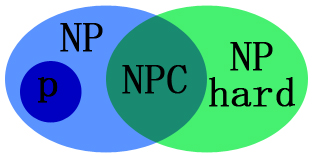
\includegraphics[width=.4\textwidth]{pics/P-NP-NPC-NP-hard.jpeg}
	\caption{P\_NP\_NPC\_NP-hard}
	\label{fig:P-NP-NPC-NP-hard}
\end{figure}



\subsection{傅里叶变换和小波分析}
傅里叶变换:知道一段时间内,信号的各个频率分量分别有多少。
小波变换:知道一段时间内,信号的各个频率分量分别有多少,以及它们都是什么时候出现的。

参考资料:\href{https://cseweb.ucsd.edu/~baden/Doc/wavelets/polikar_wavelets.pdf}{《The Wavelet Tutorial》}、\href{https://www.zhihu.com/question/22864189/answer/40772083}{如何通俗地讲解傅立叶分析和小波分析间的关系? - 咚懂咚懂咚的回答}。

\subsection{$l_1, l_2$范数对最优化问题的影响}
考虑以下优化问题:
\begin{equation}
	\begin{aligned}
		\min _{x \in \mathbb{R}^{n}} &\|x\|_{p}, \\
		\text { s.t. } & A x=b \label{eq-opt}
	\end{aligned}
\end{equation}
公式.\ref{eq-opt}中$p$表示0,1,2,$\|x\|_{p}$表示$x$的$l_p$范数。
在深度学习中,通常希望得到稀疏的解(稀疏的解,对数据的扰动也更鲁棒),即在满足约束的情况下,$x$中的非零值的数量尽可能多。咋一看,可能$l_0$范数是最符合情况的,但是$\|x\|_0$是不连续的,当$p=0$时,公式.\ref{eq-opt}就成了NP问题。当$A, b$满足一定条件时,$p=1$的时公式.\ref{eq-opt}的解也是$p=0$时的解。$l_1$范数优化问题更易求解。那么有没有更容易求解的范数呢,$l_2$可以吗?

对公式.\ref{eq-opt}进行转化:由于范数本身也是函数,该优化问题就可以视为在$A x = b$的约束下,$\|x\|_p$的最小值,从函数图像角度来看这个优化问题,就是\textbf{目标函数与约束函数的交集 --- 相交时的最小值}。

当$x \in \mathbb{R}^2$时,如Fig.\ref{fig:norm optimize}所示。
\begin{figure}[h]
	\centering
	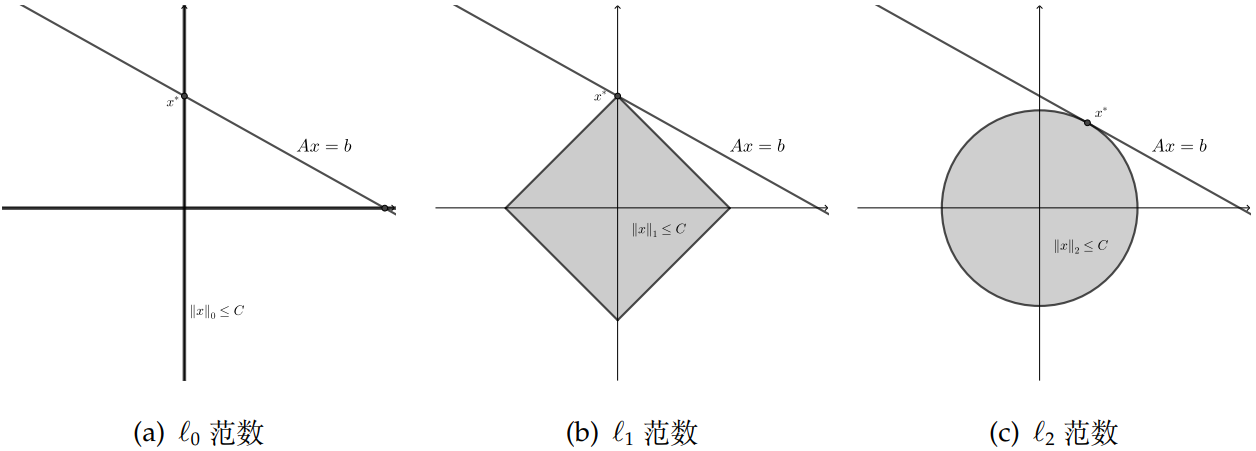
\includegraphics[width=.85\textwidth]{pics/norm optimize.png}
	\caption{$l_0, l_1, l_2$范数优化问题求解示意图}
	\label{fig:norm optimize}
\end{figure}
对$l_0$范数,$\{x | \|x\|_0 \leq 2\}$是全平面,它自然与$A x = b$相交;$\{x | \|x\|_0 \leq 1\}$退化成两条直线即坐标轴,此时问题的解就是$A x = b$与坐标轴的交点。
\begin{itemize}
	\item 对$l_1$范数,根据$C$不同,$\{x | \|x\|_1 \leq C\}$为一系列正方形,这些正方形的顶点落在坐标轴上,$A x = b$与这些正方形的交点一般是在正方形的顶点即相交于坐标轴,因此$l_1$范数的解有稀疏性
	\item 对$l_2$范数,根据$C$不同,$\{x | \|x\|_1 \leq C\}$为一系列圆,且圆有光滑的边界,圆和$A x = b$的交点可以是圆上任何一点,所以$l_2$范数优化问题一般不能保证解的稀疏性
	\item 对$l_2$范数,根据$C$不同,$\{x | \|x\|_1 \leq C\}$为一系列圆,且圆有光滑的边界,圆和$A x = b$的交点可以是圆上任何一点,所以$l_2$范数优化问题一般不能保证解的稀疏性
\end{itemize}

注意:\tbc{red}{这里目标函数与约束函数相交一般是指相切,$\{x | \|x\|_p \leq C\}$可以看成一个广义的球体,如果该球体与$A x = b$相交而不是相切,那么一定存在一个更小的$C'$使$\|x\|_p$更小且与$A x = b$相切,则$C'$成了比$C$更优的解,故一般考虑相切。}

参考资料:
\begin{itemize}
	\item《最优化:建模、算法与理论》,刘浩洋、户将、李勇锋、文再文编著,第一章,1.2
	\item \href{https://blog.csdn.net/red_stone1/article/details/80755144}{机器学习中 L1 和 L2 正则化的直观解释}
\end{itemize}


\subsection{Reparametrization}重参数化技术。参考:\href{https://spaces.ac.cn/archives/6705}{漫谈重参数:从正态分布到Gumbel Softmax}

\subsection{常用统计量}
\subsubsection{方差(Variance)} 一组数据的方差,描述的是数据与它们的均值的离散程度,衡量了这组数据的集中程度。方差可以分为样本方差和总体方差:
\begin{itemize}
	\item 样本方差:$S^2 = \frac{\sum_{i=1}^N(x_i - \bar{x})^2}{N-1}$,其中$\bar{x}$是\textbf{样本均值}
	\item 总体方差:$\sigma^2 = \frac{\sum_{i=1}^N(x_i - \mu)^2}{N}$,其中$\mu$是\textbf{总体均值}
\end{itemize}
\textbf{为什么不用要平方?}如果使用平均差($\frac{\sum_{i=1}^N |x_i - \bar{x}|}{N}$)来衡量一组数据的离散程度,可能不能很好的体现数据的分散程度(参考:\href{https://www.shuxuele.com/data/standard-deviation.html#WhySquare}{为什么要求差的平方?}),加上平方后可以放大偏离均值太远的数据的影响。也许这有点像注意力机制,在平均差中,$|x_i - \bar{x}|$的注意力值是$\frac{1}{N}$,在方差中,$|x_i - \bar{x}|$的注意力值是$\frac{|x_i - \bar{x}|}{N}$,这可以体现离均值越远的点对离散程度的贡献越大。

\subsubsection{标准差(Standard Deviation)} 标准差的平方就是方差,同理,标准差也可以分为样本std.和总总体std.:
\begin{itemize}
	\item 样本标准差:$S = \sqrt{S^2}$
	\item 总体标准差:$\sigma = \sqrt{\sigma^2}$
\end{itemize}

\subsubsection{T-statistic }


\subsubsection{p-value }

\subsubsection{t test、$\chi^2$检验}
$\chi^2$检验通常用于检验两个事件的独立性,例如可以用于分析自变量与因变量之间的独立性。如果$\chi^2$的值越大,则说明二者之间的关联性越大。

\subsection{数据的度量}
\subsubsection{定类变量}
即类别变量,其值域是某个离散的类别。能够对对象进行分类,能够判断对象之间是否同类或异类,如性别。\tbc{red}{不同类别之间没有大小关系}。

\textbf{【可以分类( $=$ 和 $\neq$),但不能排序】}

\subsubsection{定序变量}
定序变量的值不仅能够代表事物的分类,还能代表事物按某种特性的排序,但定序变量的值之间没有确切的间隔距离,\tbc{red}{只能排列出它们的顺序,而不能反映出不同值之间的距离},即不能反映一个值比另一个值大多少或小多少。如文化水平,其取值可以是文盲、小学、中学、大学等,值之间有顺序关系(如大学 $\textgreater$ 小学),但不能反映不同文化程度之间的距离。

\textbf{【可以分类( $=$ 和 $\neq$),可以排序($\textgreater$ 和 $\textless$),但不能($+$ 和 $-$ )】}

\subsubsection{定距变量}
定距变量的值之间\tbc{red}{可以比较大小,两个值的差有实际意义}。能确切测量值之间的高低、大小次序之间的距离,因而具有加与减的数学特质。但是,\tbc{red}{定距变量没有一个绝对的零点},不能乘除或倍数的形式来说明它们之间的关系。例如华氏温度:10、20、30,30比20高10,但华氏度30不是10的三倍热(\tbc{red}{0不是没有温度})。

\textbf{【可以分类( $=$和 $\neq$ ),可以排序($\textgreater$ 和 $\textless$),可以($+$ 和 $-$ ),但不能($\times$和 $\div$ )】}

\subsubsection{定比变量}
定比变量除了具有定距变量的特性外,还具有一个真正的零点,因而它具有乘与除(×、÷)的数学特质。如A的体重是60kg,而B的体重是30kg,可以算出前者是后者的两倍重,因为其零点是绝对的。

\textbf{【可以分类( $=$和 $\neq$ ),可以排序($\textgreater$ 和 $\textless$),可以($+$ 和 $-$ ),可以($\times$和 $\div$ )】}

以上四种变量类型的性质是逐渐继承的。

参考:\href{https://blog.csdn.net/YYIverson/article/details/100068865}{【统计学】区分定类、定序、定距、定比变量!!}。

\subsection{拉格朗日对偶性}
约束最优化中常用的一种方法。利用拉格朗日对偶性(Lagrange duality)将原始问题转换为对偶问题,通过求解对偶问题得到原始问题的解。

\subsubsection{原始问题}假设$f(x), g_i(x), h_j(x)$是定义在$\mathbb{R}^n$的连续可微函数。原始最优化问题为:
\begin{align}
	\mathop{min}_{x \in \mathbb{R}^n}&\quad f(x) \nonumber \\
	s.t.&\quad g_i(x) \leqslant 0, i = 1, 2, ..., k \nonumber \\
		&\quad h_j(x) = 0, j = 1, 2, ..., l \nonumber
\end{align}

引进广义朗格朗日函数:
$$
L(x, \alpha, \beta) = f(x) + \sum_{i=1}^k a_i g_i(x) + \sum_{i=j}^l \beta_j h_j(x)
$$
其中,$x \in \mathbb{R}^n$,$\alpha, \beta$是拉格朗日乘子,$\alpha_i \geqslant 0$。将$L$看作$\alpha, \beta$的函数(固定$x$),求其最大值,即:
$$
\mathop{max}_{\alpha, \beta:\alpha_i \geqslant 0} L(x, \alpha, \beta)
$$
注意,$\mathop{max}_{\alpha, \beta:\alpha_i \geqslant 0} L(x, \alpha, \beta)$表示固定$x$,$\alpha, \beta$作为变量来使$L$最大化,此时再固定$\alpha, \beta$即可得到一个关于$x$的函数:
$$
\theta_P (x) = \mathop{max}_{\alpha, \beta:\alpha_i \geqslant 0} L(x, \alpha, \beta)
$$
$P$表示原始问题。分析一下$\theta_P$:
\begin{myitemize}
	\item 当$x$违反原始约束$g_i(x) > 0$或$h_j(x) \neq 0$,则可以很容易调整对应的$\alpha_i, \beta_j$使$\theta_P(x)$取得$+\infty$。(\textbf{$\alpha_i \geqslant 0$的原因})
	\item 当$x$满足原始约束时,则有:
	$$
	\theta_P(x) = \mathop{max}_{\alpha, \beta:\alpha_i \geqslant 0} L(x, \alpha, \beta) = f(x)
	$$
	考虑$f(x) + \sum_{i=1}^k a_i g_i(x) + \sum_{i=j}^l \beta_j h_j(x)$,对于任意$x$(即固定$x$),显然有$h_j(x) = 0$,且$g_i(x) \leqslant 0$,则$\mathop{max}_{\alpha, \beta:\alpha_i \geqslant 0} L(x, \alpha, \beta)$\textbf{肯定有$\alpha_i = 0$},所以,
	$$
	\mathop{max}_{\alpha, \beta:\alpha_i \geqslant 0} L(x, \alpha, \beta) = f(x) + \sum_{i=1}^k 0 \cdot g_i(x) + \sum_{i=j}^l \beta_j h_j(x)
	$$
	即$\theta_P(x) = \mathop{max}_{\alpha, \beta:\alpha_i \geqslant 0} L(x, \alpha, \beta) = f(x)$
\end{myitemize}
因此,
$$
\theta_P(z)= \begin{cases}f(x), & x\ satisfies\ subjects \\ +\infty, & \text { otherwise }\end{cases}
$$
所以$\theta_P(x)$的极小就等价于原始问题的解,即:
$$
\mathop{min}_{x} \theta_P(x) = \mathop{min}_{x} \mathop{max}_{\alpha, \beta: \alpha_i \geqslant 0} L(x, \alpha, \beta)
$$
因此,原始不等式约束优化问题转化成了广义\textbf{拉格朗日的极小极大问题},定义原始问题的最优值:
$$
p^* = \mathop{min}_{x} \theta_P(x)
$$

\subsubsection{对偶问题}
定义关于$\alpha, \beta$的函数,
$$
\theta_D(\alpha, \beta) = \mathop{min}_{x} L(x, \alpha, \beta)
$$
$D$表示其为对偶问题,其含义可与$\theta_P$类别。考虑$\theta_D$的极大化,即:
$$
\mathop{max}_{\alpha, \beta: \alpha_i \geqslant 0} \theta_D(\alpha, \beta) = \mathop{max}_{\alpha, \beta: \alpha_i \geqslant 0} \mathop{min}_{x} L(x, \alpha, \beta)
$$
$\mathop{max}_{\alpha, \beta: \alpha_i \geqslant 0} \mathop{min}_{x} L(x, \alpha, \beta)$称为\textbf{拉格朗日函数的极大极小问题}。将朗格朗日的极大极小问题转化为优化问题:
\begin{align}
	\mathop{max}_{\alpha, \beta} \theta_D(\alpha, \beta)&\quad = \mathop{max}_{\alpha, \beta: \alpha_i \geqslant 0} \mathop{min}_{x} L(x, \alpha, \beta) \nonumber \\
	s.t.&\quad \alpha_i \geqslant 0, i = 1, 2, ..., k \nonumber
\end{align}
该问题称为原始问题的对偶问题,定义对偶问题的最优值:
$$
d^* = \mathop{max}_{\alpha, \beta: \alpha_i \geqslant 0} \theta_D(\alpha, \beta)
$$

\subsubsection{原始问题与对偶问题的关系}
若原始问题和对偶问题都有最优值,那么二者的最优值有如下关系:
$$
d^* = \mathop{max}_{\alpha, \beta: \alpha_i \geqslant 0} \mathop{min}_{x} L(x, \alpha, \beta) \leqslant \mathop{min}_{x} \mathop{max}_{\alpha, \beta: \alpha_i \geqslant 0} L(x, \alpha, \beta) = p^*
$$
\textbf{证明:}
\begin{quotation}
	$$
	\theta_D(\alpha, \beta) = \mathop{min}_{x} L(x, \alpha, \beta) \leqslant L(x, \alpha, \beta) \leqslant \mathop{max}_{\alpha, \beta: \alpha_i \geqslant 0} L(x, \alpha, \beta) = \theta_P(x)
	$$
	即,
	$$
	\theta_D (\alpha, \beta) \leqslant \theta_P (x)
	$$
	即,
	$$
	\mathop{max}_{\alpha, \beta:\alpha_i \geqslant 0} \theta_D (\alpha, \beta) \leqslant \mathop{min}_{x} \theta_P (x)
	$$
	得证。
\end{quotation}
\textbf{推论:}
\begin{quotation}
	若$x^*, (\alpha^*, \beta^*)$分别是原始问题和对偶问题的\textbf{可行解},若$d^* = p^*$,则$x^*, (\alpha^*, \beta^*)$分别是原始问题和对偶问题的\textbf{最优解}。
\end{quotation} 
那什么样的条件才满足$d^* = p^*$呢?

\textbf{Karush-Kuhu-Tucker(KKT) 条件}\label{kkt}
\begin{quotation}
	对原始问题和对偶问题,假设$f(x), g_i(x)$是凸函数,$h_j(x)$是仿射函数,并且不等式约束$g_i(x) \leq 0$是\textbf{严格可行的},即存在$x$,对所有$i$有$g_i(x) < 0$。则$x^*, (\alpha^*, \beta^*)$分别是原始问题和对偶问题的解的充要条件是$x^*, (\alpha^*, \beta^*)$满足以下KKT条件:
	\begin{align}\nonumber
		\nabla_x L(x^*, \alpha^*, \beta^*) &= 0 \nonumber \\
		\alpha_i^* g_i(x^*) &= 0, i = 1, 2, ..., k \nonumber \\
		g_i(x^*) &\leq 0, i = 1, 2, ..., k \nonumber \\
		\alpha_i^* &\geq 0, i = 1, 2, ..., k \nonumber \\ 
		h_j(x^*) &= 0, i = 1, 2, ..., l \nonumber 
	\end{align}
	
\end{quotation}

\subsection{Sequence Minimal Optimization(SMO)}\label{smo}
序列最小最优化算法,SMO是一种启发式算法,通常用于求解凸二次规划问题。

\subsection{正定核}\label{pdkf}
Positive definite kernel function。一个核函数为正定核的充要条件:
\begin{quotation}
	对任意$x_i \in \mathcal{R}, i = 1, 2, ..., m$ ,$\kappa(x_i, x_j)$对应的Gram矩阵 $[\kappa(x_i, x_j)]_{m \times m}$是半正定矩阵。
\end{quotation}

\subsubsection{常用核函数}
\begin{itemize}
	\item 多项式核:$\kappa(x, z) = (x \cdot z + 1)^p$
	\item 高斯核:$\kappa(x, z) = e^{- \frac{||x - z||^2}{2 \sigma^2}}$。为啥说高斯核等于无穷维呢?因为 $e^x$ 这个函数进行展开的话有无穷维。
\end{itemize}


\subsection{机器学习中常见的数据分布}
这里将介绍常见的一些分布,主要通过这些分布的密度函数、分布函数来介绍,以及其在机器学习/深度学习中的一些体现和应用。
\subsubsection{Gaussian}高斯分布,正态分布,钟形分布。
$$
f(x) = \frac{1}{\sqrt{2 \pi} \sigma} e^{- \frac{(x - \mu)^2 }{2 \sigma^2}}
$$
正态分布的两个参数为:$\mu, \sigma$,分别表示正态分布的均值和标准差。标准正态分布即 $\mu = 0, \sigma = 1$ 的正态分布。

\subsubsection{Laplace}拉普拉斯分布。
$$
f(x) = \frac{1}{2b} e^{- \frac{{|x - \mu|}}{b}}
$$


\subsection{变量之间的相关性检验}
在进行数据分析的时候,如果要对自变量与因变量之间的关系进行分析,或者说在多任务学习中,分析不同任务之间的相关性时,如何检验这种相关性是很重要的。

\subsubsection{Person 相关系数}
即皮尔逊相关系数,反应两个变量相似性的统计量,衡量的是两个变量之间的线性相关性,变化的趋势。定义变量 $X, Y$ 的 Person 系数为:
$$
\rho_{X, Y}=\frac{\operatorname{cov}(X, Y)}{\sigma_{X} \sigma_{Y}}=\frac{E[(X-E X)(Y-E Y)]}{\sigma_{X} \sigma_{Y}}=\frac{E(X Y)-E(X) E(Y)}{\sqrt{E\left(X^{2}\right)-E^{2}(X)} \sqrt{E\left(Y^{2}\right)-E^{2}(Y)}}
$$
其中 $\sigma$ 表示方差。皮尔逊相关系数通常衡量的是两个实值变量之间的相关性,$\rho_{X, T} \in [-1, 1]$,小于 0 表示负相关,大于 0 表示正相关,0 则表示二者不具备\textbf{线性}相关性。注意,不相关不等于独立。当 $X, Y$ 是均值为 0 的变量时,则有:
$$
\rho_{X, Y}=\frac{E(X Y)}{\sqrt{E\left(X^{2}\right)} \sqrt{E\left(Y^{2}\right)}}=\frac{\frac{1}{N} \sum_{i=1}^{N} X_{i} Y_{i}}{\sqrt{\frac{1}{N} \sum_{i=1}^{N} X_{i}^{2}} \sqrt{\frac{1}{N} \sum_{i=1}^{N} Y_{i}^{2}}}=\frac{\sum_{i=1}^{N} X_{i} Y_{i}}{\sqrt{\sum_{i=1}^{N} X_{i}^{2}} \sqrt{\sum_{i=1}^{N} Y_{i}^{2}}}=\frac{\sum_{i=1}^{N} X_{i} Y_{i}}{\|X \mid\| Y \|}
$$
显然,此时皮尔逊相关系数就成了两个向量的 $cosine$函数,即余弦相似度,再进一步,如果 $X, Y$ 的模长为 1,则皮尔徐相关系数 $\rho_{X, Y} = X \cdot Y$,即成了向量的内积。所以,其实我们也可以反推出来,向量的内积其实衡量的是向量的一种相似度,一种未归一化的相似度。

皮尔逊相关系数可以用来衡量两个用户之间的相似性,例如以两个用户对物品的评分向量计算皮尔逊相关系数。

\textbf{缺点}:
\begin{itemize}
	\item 从皮尔逊相关系数的公式可以看出,如果两个变量的配对的数据(即 $X, Y$ 都有值的数据,在评分矩阵中体现为两个用户对同一个物品进行了评分你)很少时,均值和方差的估计是不太准确的,且只有一个配对时是无法计算皮尔逊相关系数的(因为方差为 0);
	\item 没有两个变量的配对的数目的影响,即可能 $X, Y$ 之间的配对数量很大,且值也比较接近,但是如果 $X, Z$ 配对数量很小但评分基本一样,则可能 $X, Y$ 的皮尔逊相关性会小于 $X, Z$ 的相关性,这显然是不合理的;
	\item 要求变量的方差为 0,即要求变量的值是取自一个方差不为零的分布(通常假设其来自正态分布),其实从用户评分角度来看,即要求用户的偏好是可以区分的;
	\item 对绝对值不敏感,即 $X, Y$ 的趋势相似,且值的分布也比较相似,$X, Z$ 的趋势相似但 $X$ 的平均值很大,$Z$ 的平均值很小,用皮尔逊相系数衡量的话,可能 $X, Z$ 之间更相似。在推荐中,可能优的用户习惯给低分,有的用户习惯给高分; 
\end{itemize}

\subsubsection{Spearman 秩相关系数}
Spearman 秩相关系数是一种无参数(与分布无关)检验方法,用于度量变量之间联系的强弱。在没有重复数据的情况下,如果一个变量是另外一个变量的严格单调函数,则Spearman秩相关系数就是 +1 或 -1,称变量完全 Spearman 秩相关。注意这和 Pearson 完全相关的区别,只有当两变量存在线性关系时,Pearson 相关系数才为 +1 或 -1。

将 $X, Y$ 两个变量的取值看作序列,计算 $x_i$ 在 $X$ 中的顺序(秩),对于 $Y$ 计算相同的值,对于一对 $(x_i, y_i)$ 而言,秩差 $d_i$ 为 $x_i, y_i$ 的秩的差,则斯皮尔曼系数为:
$$
\rho_{s} = 1 - \frac{6 \sum_{i=1}^N d_i^2}{N(N^2 - 1)}
$$
显然,斯皮尔曼系数不仅可以度量变量之间的线性和非线性相关性,如 $y = x^2, x > 0$,用皮尔逊系数度量则为不相关的,但是在斯皮尔曼系数下可以算得二者得相关性是 1。其实,虽然斯皮尔曼不要求变量是来自某个分布得,但是可以看出它还是要求变量得值是可以比较得,否则秩就没有意义了。且要处理变量中存在重复值得情况,即在 $X$ 或 $Y$ 中存在重复值时该如何赋予秩。

当然,对于不同的变量类型,有不同得检验方法,具体可以参见:\href{https://zhuanlan.zhihu.com/p/396580986}{相关分析最全总结}、\href{https://zhuanlan.zhihu.com/p/94070722}{要做相关性分析,该如何选择正确的统计方法?}。

\subsection{Jacobean Hessian}

\subsection{指数移动平均}
指数移动平均在深度学习的梯度下降优化算法中出现的频率很高。

\section{Algorithms}
\subsection{Search}
\subsubsection{贪心算法}
贪心搜索是一种搜索解空间的策略,在搜索时,基于当前状态,选择代价最低或估计收益最大的方向作为下一步搜索的方向。使用贪心搜索并不能保证全局最优解,目的是为了找到一个可行解。在使用贪心算法前,先要证明以下两个东西:
\begin{itemize}
	\item 贪心选择性:指所求问题的整体最优解可以通过一系列局部最优的选择(通过最优度量标准来判断)来到达
	\item 最优子结构:一个问题的最优解中包含了子问题(比原问题规模更小的问题)的最优解,即每一步贪心选完后会留下子问题,子问题的最优解和贪心选出来的解可以凑成原问题的最优解
\end{itemize}
和动态规划相比,二者都需要描述清除问题的优化子结构;但是贪心算法重点是证明贪心选择的合理性,DP重点是找到子问题和合理的递推关系式。

典型的贪心问题:Huffman编码、活动选择问题。



\subsubsection{Beam Search}
也叫集束搜索。
对贪心搜索的一种改进。在进行搜索时,并不是只沿一个方向搜索,会同时保留$n$个最优的方向,分别以这$n$个方向进行扩展,扩展后在每个方向都可以得到$n$个备选项,那么则有$n^2$个备选项,在这$n^2$个被选项里选择最优的$n$个备选项作为下次扩展的方向,以此类推,即在搜索树的每一层都只保留$n$个方向。$n$就是beam width。




\section{\LaTeX}
\subsection{在pdf中嵌入代码}在\LaTeX 中嵌入代码有多种方法。可以使用的包有:listings、minted、tcolorbox等方式。

\subsection{参考文献相关}
\paragraph{引入参考文件}引入参考文献时,可以使用.bib文件的方式引入参考文件。写好.bib文件后,需要按序执行以下四步完成引用:
\begin{enumerate}
	\item 先编译.tex文件。个人认为是编译.tex文件,为参考文献产生位置
	\item 编译.bib文件(一般使用bibtex),生成编译后的参考文献
	\item 再编译.tex文件,这时会将参考文献引入到.tex编译后的文件中(好像是.aux文件)。但这时在正文中可能不会正常显示
	\item 再次编译.tex文件即可得到引用正确、显示正确的pdf
\end{enumerate}

\subsection{数学符号}
\paragraph{数学字体}其中某些单元格的内容可能出错了,只需要把多余的字符去掉即可。
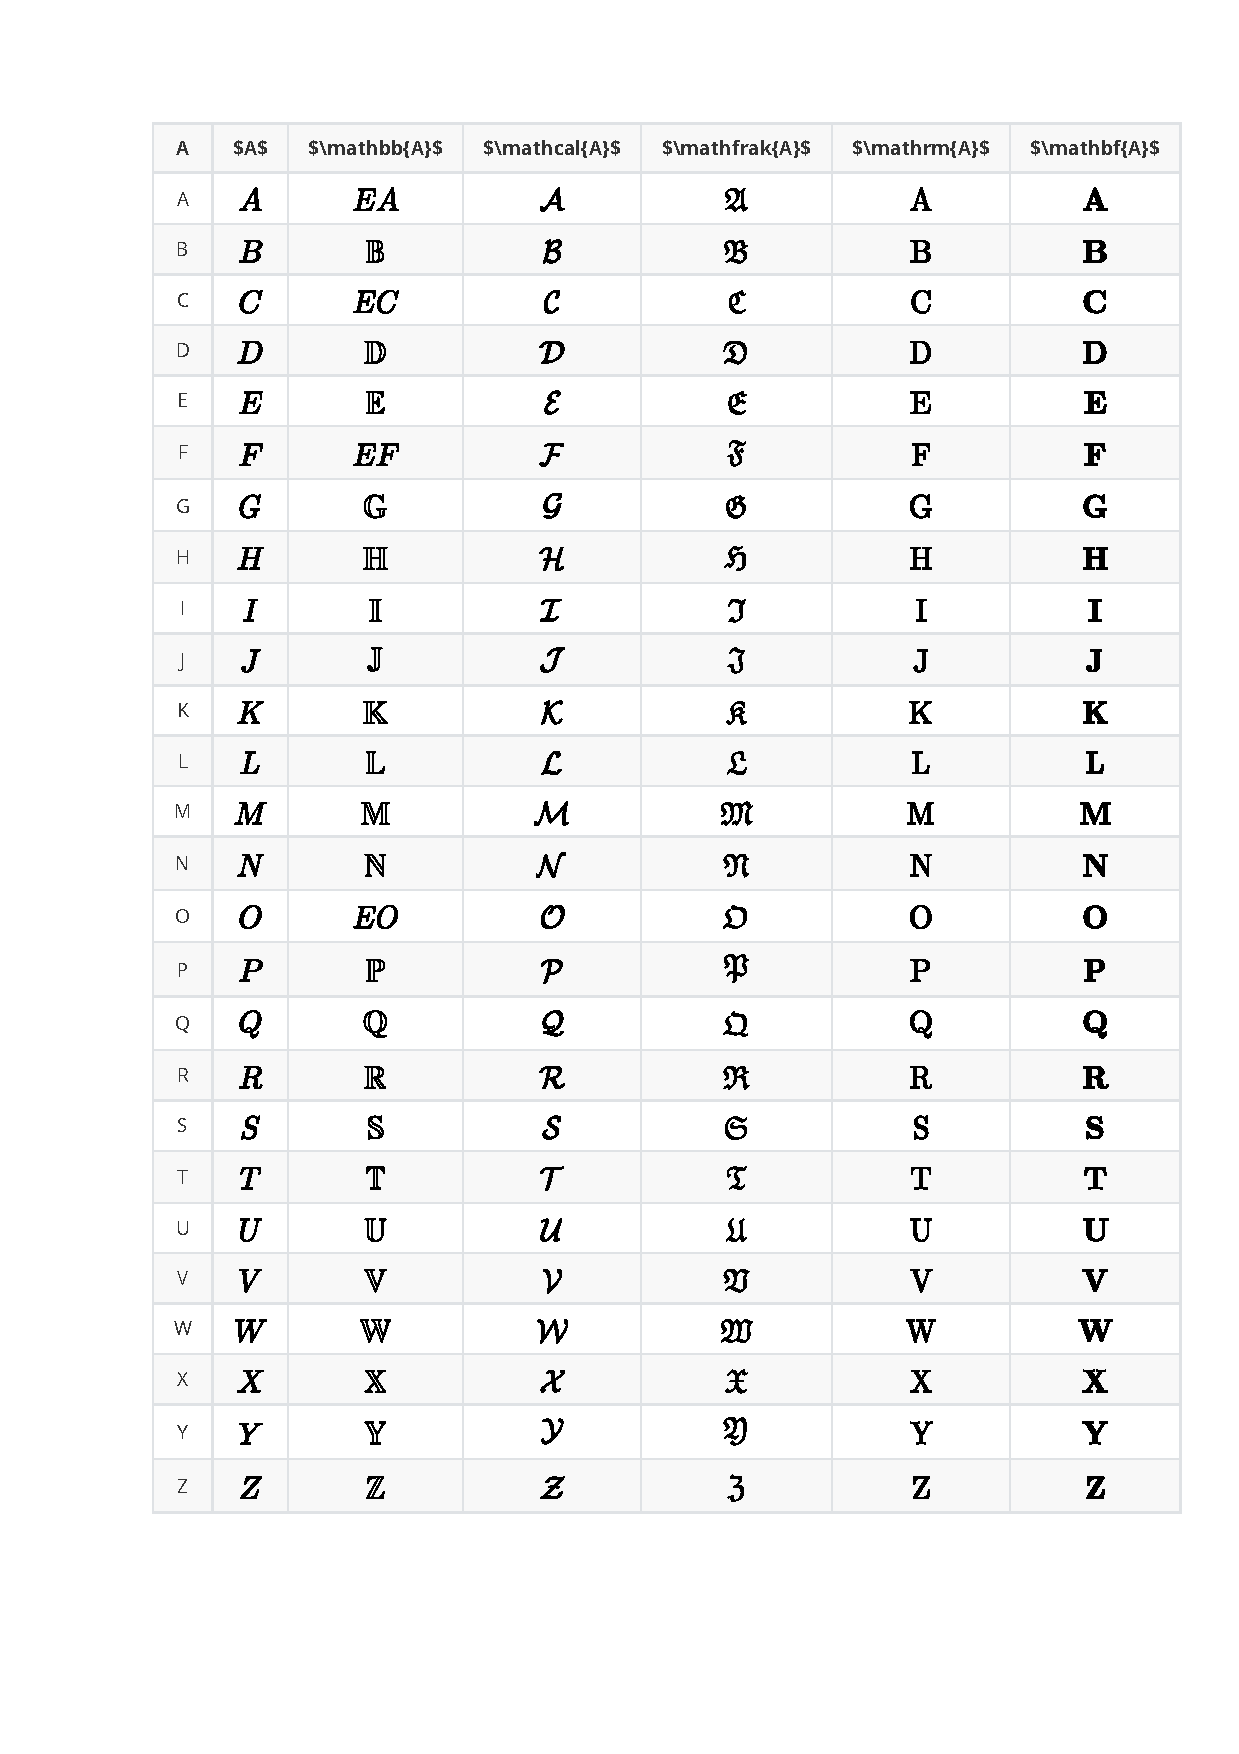
\includepdf{mathfonts.pdf}

\subsection{\LaTeX 中的颜色}
参考\href{http://latexcolor.com/}{latexcolor}。

\subsection{注脚}
两种常用形式:
\begin{itemize}
	\item \begin{verbatim}\footnote{注脚的内容}\end{verbatim}
	\item 这种方式很方便,可以在多处共享一个注脚,只需使用同一个注脚编号即可
	\begin{verbatim}
		\footnotemark[注脚编号]
		\footnotetext[编号]{注脚内容}
	\end{verbatim}
\end{itemize}

\subsection{章节编号}
默认是从1开始编号的,如果要从0开始,可以加一条命令:\begin{verbatim}\setcounter{section}{-1}\end{verbatim}










\section{Coding}

\subsection{C++}
参考文档: \href{https://www.cplusplus.com/}{cplusplus.com}
\subsection{C++数据类型转换}
\paragraph{数字 <=> 字符串}
\begin{itemize}
	\item itoa: 整数转为字符串, 可以设置基底
	\item stoi: 字符串转为整数 , 可以设置基底
	\item atoi、atol、atoll: 将字符串转为int/long/long long, 可以设置基底
	\item to\_string: 可以讲数字转为字符串, 包括整数、小数等
\end{itemize}

\subsection{C++集合} 通过$\#include<set>$来引入set. 关于集合的一些运算, 包含在algorithm库中. 在algorithm库中有一个includes函数, 可以用来判断两个容器之间是否存在包含关系, 但是, 要注意\tbc{red}{两个容器都要先从小到大进行排序!!!}
\begin{cpp}
	// 省略头文件和库的包含代码
	int container[] = {5,10,15,20,25,30,35,45,50};
	int continent[] = {40,30,20,10};
	
	sort (container,container+10);
	sort (continent,continent+4);
	
	// using default comparison:
	if ( std::includes(container,container+10,continent,continent+3) )
		cout << "container includes continent!\n";
	else	cout<<"NO\n";
	
\end{cpp}


\subsection{字符串}
C++中字符串用双引号括起来, 字符用单引号括起来. 
\paragraph{字符串比较}
compare

\paragraph{常用方法}
\begin{itemize}
	\item 初始化: \mintinline{cpp}{string s(n, 'c');}
	\item 插入字符串: \mintinline{cpp}{s.insert(pos, len, "insert");}
	\item 删除子串: \mintinline{cpp}{s.erase(pos, len, "erase");}
	\item 
\end{itemize}

\subsection{数组}
\paragraph{数组初始化}
\begin{itemize}
	\item \mintinline{cpp}{type [][depth][depth]...[depth]}声明多维数组时, 只能有一维的大小不指定
	\item \mintinline{cpp}{int arr[5] = {1, 2, 3, 4, 5}}声明数组时可以给数组赋值(初始化列表), 如果指定的数组大小则$\{\}$中的值的数量应该小于等于数组大小, 如果数量小于数组大小, 则数组中后续位置将会被填充默认值(对于基础类型, 则为0). 因此, 当$\{\}$未空时, 数组将会被填充为默认值
	\item \mintinline{cpp}{int *p = new int[5]}将在堆中分配内存, 此时也可以对数组进行初始化: \mintinline{cpp}{int *p = new int[]{1, 2, 3, 4, 5}}、\mintinline{cpp}{int *p = new int[]()}. 对于基本类型, 如果不进行初始化, 局部定义的数组的值是未定义的;对于类类型, 会默认调用其默认构造函数. \textbf{堆中分配的数组要用delete删除}
\end{itemize}

\subsection{遍历vector的方式}
\begin{cpp}
	vector<int> nums = {1, 2, 3, 4, 5};
	// 方法1: 下标
	for(int i = 0; i < nums.size(); i++){
		// do something
	}
	
	// 方法2: 迭代器
	for(vector<int>::iterator it = nums.begin(); it != nums.end(); it++){
		// do something
	}

	// 方法3: auto, 以引用的形式遍历, 可以修改值
	for(auto &it: nums){
		// do something 
	}

	// 方法4: auto, 以值的形式遍历, 不可以修改值
	for(auto it: nums){
		// do something
	}
	
	// 方法5: for_each
	foreach(nums.begin(), nums.end(),
			[](const auto &val) -> void { 
				// do something
			})
	
\end{cpp}

\subsection{for\_each}
for\_each源码如下: 
\begin{cpp}
	template<class InputIterator, class Function>
	Function for_each(InputIterator first, InputIterator last, Function fn)
	{
		while (first!=last) {
			fn (*first);
			++first;
		}
		return fn;      // or, since C++11: return move(fn);
	}
\end{cpp}
其中参数fn是一个一元函数(即只能有一个参数), 它的返回值会被忽略. 

\subsection{deque}
\mintinline{cpp}{#include <deque>}. double ended queue, 双端队列. \href{https://www.cplusplus.com/reference/deque/deque/?kw=deque}{dequ}e是一种动态容器(通常以动态数组的形式, 如链表, 来实现), 可以在两端增加或者删除元素, 随机访问deque中的元素. 

\subsection{priority\_queue}
\mintinline[bgcolor=yellow]{cpp}{#include <queue>}. 
\begin{minted}{cpp}
	template <class T, class Container = vector<T>,
	class Compare = less<typename Container::value_type> > class priority_queue;
\end{minted}
\href{https://www.cplusplus.com/reference/queue/priority_queue/?kw=priority_queue}{priority\_queue}, 优先队列. priority\_queue是一种容器适配器(container adaptor), 它使用某种容器(可以是queue、vector等, 默认是vector)作为其数据的容器, 并提供了一些接口来访问容器内的元素, 重点就在这些接口上(\mintinline{cpp}{push, pop, top})!priority\_queue的特点: 
\begin{myitemize}
	\item 第一个元素是优先级最大/小的元素(大/小根堆)
	\item \mintinline{cpp}{top} : 返回顶部的元素, 即优先级最大/最小的元素
	\item \mintinline{cpp}{pop} : 删除顶部的元素
\end{myitemize}
例子: 
\begin{minted}[linenos, breakafter=true,autogobble=true,frame=leftline]{cpp}
	#incldue <queue>
	
	int main(){
		// 大根堆
		priority_queue<int> a; // <=> priority_queue<int, vector<int>, less<int> >a
		
		// 小根堆
		priority_queue<int, vector<int>, greater<int> > b;
	}
\end{minted}




\subsection{Python}
\subsection{basics}
\subsubsection{defaultdict} python中的defaultdict,也是一种dict。与传统的dict不同,当传统的dict的key不存在时会Error,但defaultdict不会,而是返回一个默认值。该默认值由创建defaultdict时传入的参数有关:$dd = defaultdict(default_factory)$。

当default\_factory是list时,默认值是[],defaultdict其他常见取值还有:str, set, int, dict。但不可以是defaultdict。

\subsubsection{glob} python中的一个内置模块,用于查找符合特定规则的文件路劲。如:
\begin{python}
	import glob
	pattern = "./myfloder/prefix-*.txt"
	li = glob.glob(pattern) # 此时li中就包含了所有符合pattern这个模式的文件名
\end{python}

\subsubsection{python format用法}
\textbf{对齐}"$\{:\}$" 通常将对齐符号放在$:$后。\^ 、| < | >分别是居中、左对齐、右对齐,在填充符号后面可带宽度,在$:$后可带填充字符,默认为空格。

\subsubsection{数字输出格式}主要包括小数位数(如.2f)、百分号输出(如.2\%)、指数形式输出(如.2e)、带正负符号的输出(如+.2f)、按不同进制的输出(b、d、o、x分别是二进制、十进制、八进制、十六进制,在b|o|x前加\#可以输出进制符号,x的大小写会影响进制符号的大小写。
\begin{python}
	"{:^8}".format("居中")	# 居中显示,宽度为8,默认用空格填充
	"{:*<8}".format("左对齐")	# 左对齐显示,宽度为8,用*填充
	"{:*>8}".format("右对齐")	# 右对齐显示,宽度为8,默认用空格填充
	"{:.2f}".format(123)
	"{:.2%}".format(123)
		"{:^8.2f}".format(123)		# 八位的显示宽度,保留2位小数
		"{:b}".format(11)
		"{:d}".format(11)
		"{:o}".format(11)
		"{:x}".format(11)
		"{:#x}".format(11)
		"{:#X}".format(11)
	\end{python}


\subsection{numpy}
\subsubsection{np.argsort} 对数组的元素进行排序(默认是从小到大),生成一个新的数组,数组元素是排序后的数组所对应的下标。
\begin{python}
	import numpy as np
	x = np.array([2,1,3,5,4])
	y = np.argsort(x) # y = [1, 0, 2, 4, 3]
	# 从大到小排序
	y = np.argsort(-x) # y = [3, 4, 2, 0, 1]
\end{python}
该方法还有更复杂的使用方法,可以根据参数进行调节,$argsort(a, axis=-1, kind=None, order=None)$。

\subsubsection{numpy设置随机数种子} $np.random.seed(seed)$。





\subsubsection{numpy nan的处理}numpy中可以使用np.isnan()来判断数组中的元素是否为NAN,返回的结果与数组形状相同,元素为True/False,该位置的元素为NAN是则为True,否则为False。可以使用 np.nan\_to\_num(x, copy=True, nan=0, posinf= 1.7976931348623157e+308, neginf=-1.7976931348623157e+308) 来进行转换。该函数可以将NAN(包括无穷小、无穷大)转换为数字,可以指定转换后的数字。参数:x是待转换的数据,可以是数组或单个数字;copy表示是否进行原地转换,相当于pandas中的in\_place参数,但取值与in\_place相反;nan表示取代NAN的数字;posinf、neginf表示用什么取代正/负无穷。

\subsubsection{找到数组中nan指的位置}:np.argwhere(np.isnan(a))。解释:通过np.isnan标记数组中nan值的位置为True,np.argwhere会返回那些True的下标。


\subsection{matplotlib}
\subsubsection{matplotlib中的marker}如图\ref{fig:matplotlib-markers}所示,更多内容可参见:\href{https://matplotlib.org/api/_as_gen/matplotlib.pyplot.plot.html#matplotlib.pyplot.plot}{Matplotlib}
\begin{figure}[h]
	\centering
	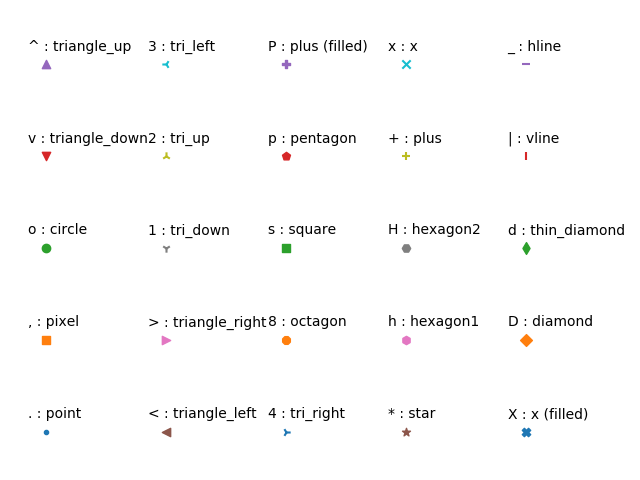
\includegraphics[width=.65\textwidth]{pics/markers.png}
	\caption{Matplotlib中的markers}
	\label{fig:matplotlib-markers}
\end{figure}

\subsubsection{Animation}
Animation可用于制作动画。初始化函数:
\begin{python}
	def __init__(self, fig, func, frames=None, init_func=None, fargs=None,
	save_count=None, *, cache_frame_data=True, **kwargs)
	"""
	fig: 绘制动画的地方
	func: 完成动画动作的回调函数。定义应为:def func(frame, *fargs) -> iterable_of_artists
	frames: 可以认为是每一个动画帧的索引,通常为iterable对象,frames中的每个值会逐个作为func的第一个参数传入
	init_func: 在绘制第一帧之前调用的函数,定义应为:def init_func() -> iterable_of_artists
	fargs: 用于func的额外的参数
	repeat_delay: 帧之间的延迟,单位为毫秒
	repeat: 是否重复播放动画
	blit: 布尔值故, 默认为False。用于优化绘图,注意这个参数有点坑,当其为True时,会根据artists的zorder来绘图,当对象没有zorder(如bar)时则会报错
	"""
\end{python}
在使用matplotlib制作动画的过程中,很重要的是要知道要让什么对象发生变化、发生什么变化 --- 知道了这二者之后就可以在每一帧的更新函数中完成对应的动作了。

\tbc{red}{注意}:blit参数的使用,当启用了blit时,且要对bar改变时,则会报错:\textit{AttributeError: 'BarContainer' object has no attribute 'get\_zorder'},把blit设为False即可。


\subsubsection{调整子图间距}
\begin{itemize}
	\item plt.tight\_layout()
	\item plt.subplot\_adjust(left=None, bottom=None, right=None, top=None, wspace=None, hspace=None)
\end{itemize}

\subsubsection{显示中文}
\begin{python}
	plt.rcParams['font.sans-serif'] = ['SimHei'] # 步骤一(替换sans-serif字体)  
	plt.rcParams['axes.unicode_minus'] = False  # 步骤二(解决坐标轴负数的负号显示问题)
\end{python}

\subsection{python中的线程有什么问题?怎么解决?}
python 中有一个叫 GIL(Global Interpreter Lock,全局解释器锁) 的玩意儿,每个线程想要执行必须先获取到这把锁,不管你 CPU 有几个核心,锁只有一把。所以每次只能有一个线程在执行。

\subsection{有序数组中找到一个数字的插入位置}
 





\subsection{Tensorflow/PyTorch}
\subsection{tf.variable\_scope \& tf.name\_scope}

\subsection{tf.sparse\_tensor}	tf中的稀疏张量。使用三个稠密的张量来表示。
\begin{itemize}
	\item indices: 表示原张量中非零值的位置
	\item values: 表示indices中元素所指位置上的值
	\item dense\_shape: 表示原张量的shape
\end{itemize}

\subsection{tf.train.Saver}tf中用于保存、恢复模型参数的接口。主要由两个接口:1)tf.train.Saver().save()用于保存模型;2)tf.train.Saver().restore()用于回复模型。
\begin{python}
	import tensorflow as tf
	saver = tf.train.Saver(max\_to\_keep=3) # max\_to\_keep表示保存的checkpoint最大次数
	...
	# 保存模型
	# sess: 会话的名字
	# save\_path: 模型的保存路径
	# global\_step: 保存模型时的后缀
	# 使用以下方法保存模型后会产生四个文件,分别是:
	# checkpoint文件:会记录最新的模型是哪个
	# .ckpt.meta文件:包含元图,保存了计算图的结构,没有变量的值
	# .ckpt.data 文件:保存权重等参数
	# .ckpt.index 文件:为数据文件提供索引,{还不太确定}
	saver.save(sess=sess, save_path=model_save_path, global_step=step)
	...
	# 恢复模型
	# save_path可以不用加模型的后缀
	saver.restore(sess=sess, save_path=model_save_path)
\end{python}

\subsection{tf.Session}运行tf中操作的类,Session类封装了运行操作所需要的环境。可以使用手动开启和关闭、上下文的方式使用Session。在使用Session时还可以进行配置,将配置作为Session初始化的参数传入。

\subsection{tf中的RNN}RNN的训练数据与其他神经网络的训练数据有一点不一样。通常的NN中的训练数据,每个样本就是一个向量。但是在RNN中,每个训练样本就是一个矩阵,每一行表示一步的输入,正因为RNN所处理的问题不同,RNN的输出数据也变得更加复杂。\\
针对不同的RNN有不同形式的输出,但可以进行简单的归纳:对于RNN中的每个样本,其形式为$\mathbb{R}^{max\_time \times embed\_size}$,其中$max\_time$表示所有样本中序列的最大长度,$embed\_size$表示每一步的输入的长度。当输入了一个样本后,会将样本的每一行 --- 即每一步的数据输入到RNN中,由于RNN本身的特点,每一步都可以产生输出,通常来说包含每一步的输出和状态(具体到不同的RNN时会有不同)。每一步的输出维度会收到RNN模型隐层宽度 --- 即隐层单元数量的影响。并且针对不同的任务,最终需要的输出是不一样,例如m对n、m对1、m对m的任务等等。\\
在tf中,有多种关于RNN单元的类,如BasicLSTMCell、GRUCell、MultiRNNCell。可以在这些类的基础上搭建自己的RNN模型。


\subsection{ImageDataGenerator}
这是Keras中的一个图像数据生成器,同时也可以在batch中对数据进行增强,扩充数据集大小,增强模型的泛化能力。比如进行旋转,变形,归一化等。

\subsection{tf.where}
tf.where(condition, x=None, y=None, name=None)

condition是一个布尔数组,condition、x、y的维度必须相同。

其中x、y可以为None,此时返回的是一个二维数组,该二维数组的行数表示condition中为True的元素的数量,每一行代表对应为True元素的坐标。

当x、y不为None是(x,y必须同时不为None),则会创建一个与condition同样shape的张量,该张量某位置的元素的取值来自x或y,当该位置在condition中为True是则来自x,否则来自y。


\subsection{TFRecord}
下列表来自\href{https://www.jianshu.com/p/72596a8488c3}{简书}:
\begin{itemize}
	\item Record顾名思义主要是为了记录数据的。
	\item 为了更加方便的建图,原来使用placeholder的话,还要每次feed\_dict一下,使用TFRecord+ Dataset 的时候直接就把数据读入操作当成一个图中的节点,就不用每次都feed了。
	\item 可以方便的和Estimator进行对接。
	\item TFRecord以字典的方式进行数据的创建。
\end{itemize}

\subsection{tf.Graph}
不同Graph之间的变量是不可以共享的!


\subsection{tf.pad}
这是tf种对tensor进行填充的函数。\textit{tf.pad(tensor, paddings, mode='CONSTANT', constant\_values=0, name=None)}。其中tensor为要被填充的张量;paddings表示填充时要填充多少值进去,控制了填充后tensor的大小;mode表示填充的模式,什么样的值被填充进去;constant\_value表示mode为CONSTANT时的常量值。其中最重要的参数是\textit{paddings}。\textit{paddings}是一个形状为[n,2]的tensor,n为input的rank(其实可以简单理解为len(input.shape))。\textit{paddings}中的第$i$个元素可以看做是一个长度为2的数组,第一个元素表示了在input的第$i$维的前面增加的大小,第二个元素表示在第$i$维的后面增加的大小,那么对于input的第$i$来说,它的大小较原来增大了$paddings[i][0]+paddings[i][1]$。

\subsection{tf.tile}平铺张量。\textit{tf.tile(input, multiples, name=None)}。其中input是一个张量;multiples是一个1-D数组,数组的长度是input的维度数量,每个元素的值表示input被复制的次数,即\textit{input.dims[i] = input.dims[i] * multiples[i]}。

\subsection{tf.squeeze}压缩张量,将张量中维度大小为1维压缩掉。

\textit{tf.squeeze(input, axis=None, name=None)}。

input为输入的张量;axis为可选参数,可以为整数或者整数1-D数组,为None时表示移除所有大小为1的维,否则移除指定的维。

反之则为$unsqueeze$。

\subsection{tf.expand\_dims}给数据增加维度。\textit{tf.expand\_dims(input, axis, name)},表示在$input$的第$axis$维插入一个维度,维度大小为1。



\subsection{ML/DL错误集锦}
\paragraph{batch\_size对训练的影响}

\paragraph{某个iteration成为训练效果的短板}

\paragraph{损失函数值为NaN}

\paragraph{\tbc{red}{类别的正负样本不均衡问题}}

\paragraph{数据的格式问题}

%\section{IDEAS}
%\subsection{Ideas01}
%% 记录日常的一些想法
\paragraph{基于深度神经网络的模型也可以看作是一种图,能否使用gml的一些方法对其进行分析?} 很可惜,这个想法已经被发表成论文了\cite{you2020graph}。

但是这方面地工作还比较少,可以做的方向有:
\begin{itemize}
	\item 如何对Deep neural network进行建模,现在地DL模型中,有着众多的变化,如网络中的DROP技术、pooling、随着训练单元之间的连接权重变化等
	\item {\color{red}神经网络模型的训练会随着训练发生变化,能否将其视作动态图?}
	\item 对深度网络建模后,对其进行分析,分析其具有何种性质,与现有的网络常识、规律进行比较
	\item 能够通过对深度网络的分析,得到神经网络所蕴含的更高层的语义,对模型进行解释?
	\item 能否通过对深度神经网络的分析对深度模型进行改善?
\end{itemize}

\paragraph{生物的大脑中的神经元之间互相联系,也可以看作一种图,能否以研究图的一些方法对大脑的神经系统进行研究?} 已经有相关的论文了!!!
\paragraph{将代码视作图}	已经有相关论文。数据集 LINUX \cite{6228085} 内核中的程序依赖图,每个图代表一个函数,每个结点代表一条语句,边表示语句之间的依赖。
\paragraph{找到科研新点子的方法} 纵览研究领域,看看传统方法都是怎么解决领域内的主要问题的,或者解决了一些什么问题,再看看传统方法的局限性,或者如何用新的方法解决领域内的问题。
\paragraph{图领域一些难点,未解决的问题}\newline
1. 影响力最大化问题
2. 影响力问题中对negative influence的考虑


\paragraph{武林外传(my own swordsman}\\
1. 吃再多苦,只当自己是二百五;受再多罪,只当自己是窝囊废 
2. 只要给够加班费,当牛做马无所谓

\paragraph{神经网络中的一些点子}\\1. 设计新的神经单元
2. 设计新的网络结构
3. 开发更有效的正则化策略

\paragraph{从图的表征中重建图} 是否能够从图的表征或者图中所有结点的表征为基础来重建传统的图的结构$G = (V, E) $。这样的重建可以作为图数据的一种加密方式、图数据的压缩保存等。GraphRNN\cite{you2018graphrnn}中的图生成,反过来是否能看作从表征重构图的过程?{\color{red}更准确的讲,这应该叫图地编码解码!}

对于图的编码解码,已经有相关的工作\cite{simonovsky2018graphvae},但这方面的工作还比较少。

\paragraph{自动文献调研} 给定一个领域限定,能够自动地调研相关领域地资料(文献,网路资源),能够在调研后发现问题新的解决方法,或者挖掘出新的问题。那能否完成\textbf{自动写论文呢}\cite{wang-etal-2019-paperrobot}?(自动文档摘要可以作为这样的一个系统的一部分)

\paragraph{基于多层次的图相似性计算}从输入的图,生成每个图的多层级表示,在多个层级的表示上进行相似度计算。这方面现在已经有一些相关的工作,不过还比较少。多个层级的划分可以基于以下的标准:
\begin{itemize}
	\item 可以基于不同的表示粒度,如结点、超点、图的表征
	\item 使用不同的方法来获得不同层次的表示
	%\item 
\end{itemize}
在计算图的相似度时主要有这么几个难点:
\begin{itemize}
	\item 图的同构性问题。一个图的结点排列是不确定的,基于不同的结点排列可能会有不同的表示
	\item 要是inductive的。能够泛化到未见过的图
	\item 能对大图进行相似度的计算。由于图的规模一大,对其进行比较将会是一件耗时的操作
	\item {\color{red}图数据的丰富性}。例如多重图、有向图、异构图、知识图谱等
	\item {\color{red}动态图}。其实,目前大部分工作是在静态图上开展的,如何现有研究工作扩展到动态图还有很大的研究空间
\end{itemize}


\paragraph{在结点表征的基础上做一些延申性的工作}比如链接预测、动态的链接预测等。
g
\paragraph{针对图数据库,基于图相似性的图表征}在一个很大的图数据库中,如果我们得到了任意两个图之间的相似性,能否利用相似性来计算图的表征呢?这个想法源于:基于邻居信息聚合的结点的表征是利用结点之间的关系(可以认为是相似性)来聚合邻居结点信息。那么,{\color{red}在一个很大的图数据库中,能否构造一个超图,利用图之间的相似性构造一个这样的超图呢?,每一个图数据作为超图中的点,边可以以图之间的相似性来构建。在这样的一个超图的基础上来学习图的表征?}在这个想法中,关键之处在于相似性如何得到,现有的一些图相似性的计算就是基于图的表征来计算的,那这样不就是多此一举了吗?

\paragraph{GNN生成的表征空间的问题}对于使用不同的GNN/GCN生成的结点/图表征,它们之间存在什么样的关系呢?是否会受到数据本身的影响呢?比如一个GNN将一个图中的所有结点映射到一个向量空间中,另一个GNN把所有结点映射到另一个向量空间中,这两个空间会存在某种关系吗,存在什么样的关系呢?{\textbf{\color{red}这种关系是否反映了不同GNN模型之间的关系呢?}}




% %一 \section{Task description and data construction}
% \label{sec:headings}

%\subsection{Headings: second level}
% \begin{equation}
% \xi _{ij}(t)=P(x_{t}=i,x_{t+1}=j|y,v,w;\theta)= {\frac {\alpha _{i}(t)a^{w_t}_{ij}\beta _{j}(t+1)b^{v_{t+1}}_{j}(y_{t+1})}{\sum _{i=1}^{N} \sum _{j=1}^{N} \alpha _{i}(t)a^{w_t}_{ij}\beta _{j}(t+1)b^{v_{t+1}}_{j}(y_{t+1})}}
% \end{equation}



% \section{Examples of citations, figures, tables, references}
% The documentation for \verb+natbib+ may be found at
% \begin{center}
%   \url{http://mirrors.ctan.org/macros/latex/contrib/natbib/natnotes.pdf}
% \end{center}


% \begin{verbatim}
%   \citet{hasselmo} investigated\dots
% \end{verbatim}

% \begin{quote}
%   Hasselmo, et al.\ (1995) investigated\dots
% \end{quote}

% \begin{center}
%   \url{https://www.ctan.org/pkg/booktabs}
% \end{center}

% 引用表格
% 需要给表格加上标签,格式:\label{fig:fig1}
% \ref{fig:fig1}

% \subsection{Figures}
% 123123
% See Figure \ref{fig:fig1}. Here is how you add footnotes. \footnote{Sample of the first footnote.}
% 123123

% \begin{figure}
%   \centering
%   \fbox{\rule[-.5cm]{4cm}{4cm} \rule[-.5cm]{4cm}{0cm}}
%   \caption{Sample figure caption.}
%   \label{fig:fig1}
% \end{figure}


% 表格
% \subsection{Tables}
% 1312
% See awesome Table~\ref{tab:table}.

% \begin{table}
%  \caption{Sample table title}
%   \centering
%   \begin{tabular}{lll}
%     \toprule
%     \multicolumn{2}{c}{Part}                   \\
%     \cmidrule(r){1-2}
%     Name     & Description     & Size ($\mu$m) \\
%     \midrule
%     Dendrite & Input terminal  & $\sim$100     \\
%     Axon     & Output terminal & $\sim$10      \\
%     Soma     & Cell body       & up to $10^6$  \\
%     \bottomrule
%   \end{tabular}
%   \label{tab:table}
% \end{table}



% 打印参考文献
\printbibliography
\bibliographystyle{plain}
\bibliography{references}



\end{document}
